\chapter{Extending Reinforcement Learning in Diffusion Models}



This chapter builds upon the existing diffusion framework by exploring the utility of intermediate state rewards rather than relying solely on the final outcome of the trajectory. An empirical analysis is conducted on the reward signal dynamics throughout the denoising process using trajectories from the 
\href{https://huggingface.co/google/ddpm-celebahq-256}{\texttt{\texttt{google/ddpm-celebahq-256}}} model. The focus is on understanding the value of these intermediate rewards and exploring algorithmic extensions. Additionally, the work replicates aspects of \textit{``Training Diffusion Models with Reinforcement Learning''} \cite{black2023training} using a pretrained DDPM model on the CelebA-HQ 256 dataset \cite{karras2017progressive}, testing three of the four tasks from the original study and introducing an additional task, OVER50. Model checkpoints and training dynamics are made available for further investigation and comparison (see Appendix~\ref{appendix:implementation}). 

% Visual comparison between pretrained and ckpts fintuned with DDPO
\begin{figure}[ht]
  \centering
  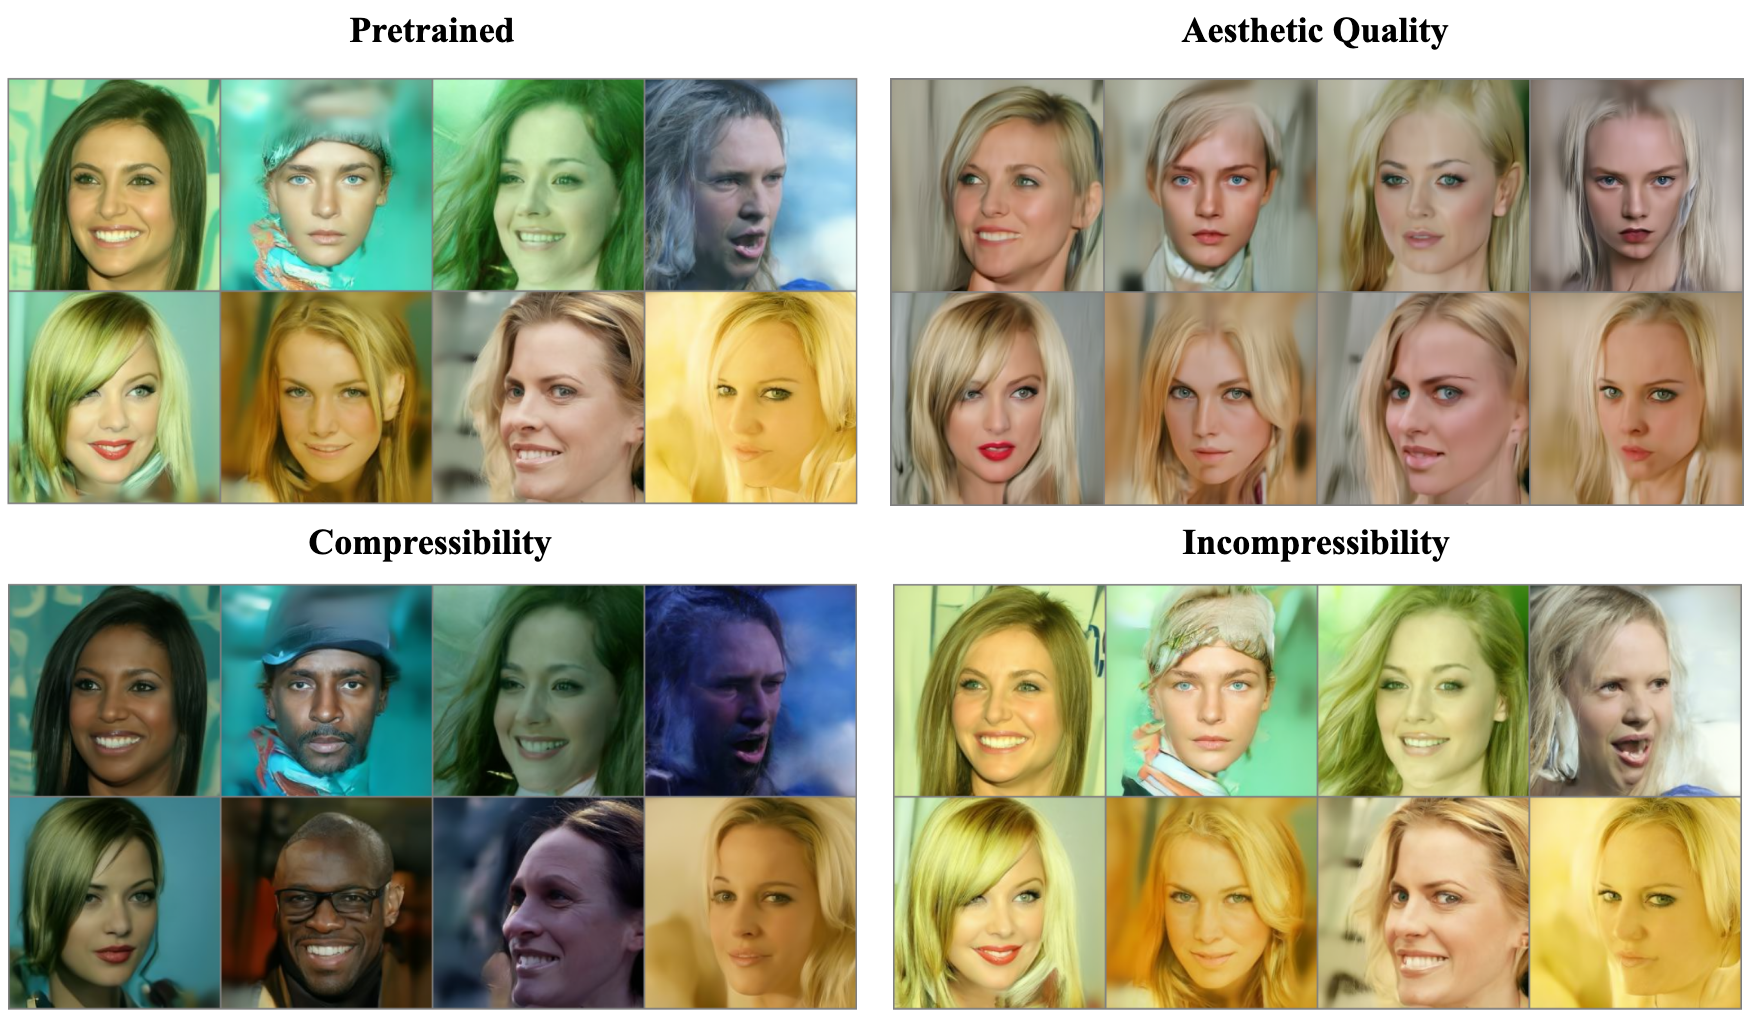
\includegraphics[scale=0.72]{img/results/visual-comparison-results-200dpi.png}
  \vspace{-4pt}  % reduce space between caption and figure
  \captionsetup{width=\textwidth} % set the width of the caption
  \caption{\textbf{DDPM pretrained model's samples vs DDPO finetuned samples.} Qualitative depiction of the effects of RL finetuning on different reward functions using \href{https://huggingface.co/google/ddpm-celebahq-256}{\texttt{\texttt{google/ddpm-celebahq-256}}}
  pretrained model. Additional samples are provided in Appendix~\ref{appendix:additional-celebahq-samples}.}
  \label{fig:visual-comparison-ddpo}
\end{figure}

% Our contributions extend the existing framework of the diffusion process by exploiting the informative intermediate state rewards rather than solely relying on the final trajectory outcome. We analyze the reward signal dynamics throughout the denoising process using a collection of sample trajectories from the \textit{google/ddpm-celebahq-256} model. Additionally, we propose extended reward functions that incorporate further information beyond the final sample, alongside the introduction of baseline functions during RL training. Model checkpoints are provided for each of the proposed methods, allowing for further exploration and comparison (see Appendix~\ref{appendix:implementation}). \\

\section{Diffusion Model as Sequential Decision making Process}\label{sec:diffusion-model-mdp}

% Diffusion Model as MDP
\begin{figure}[ht]
  \centering
  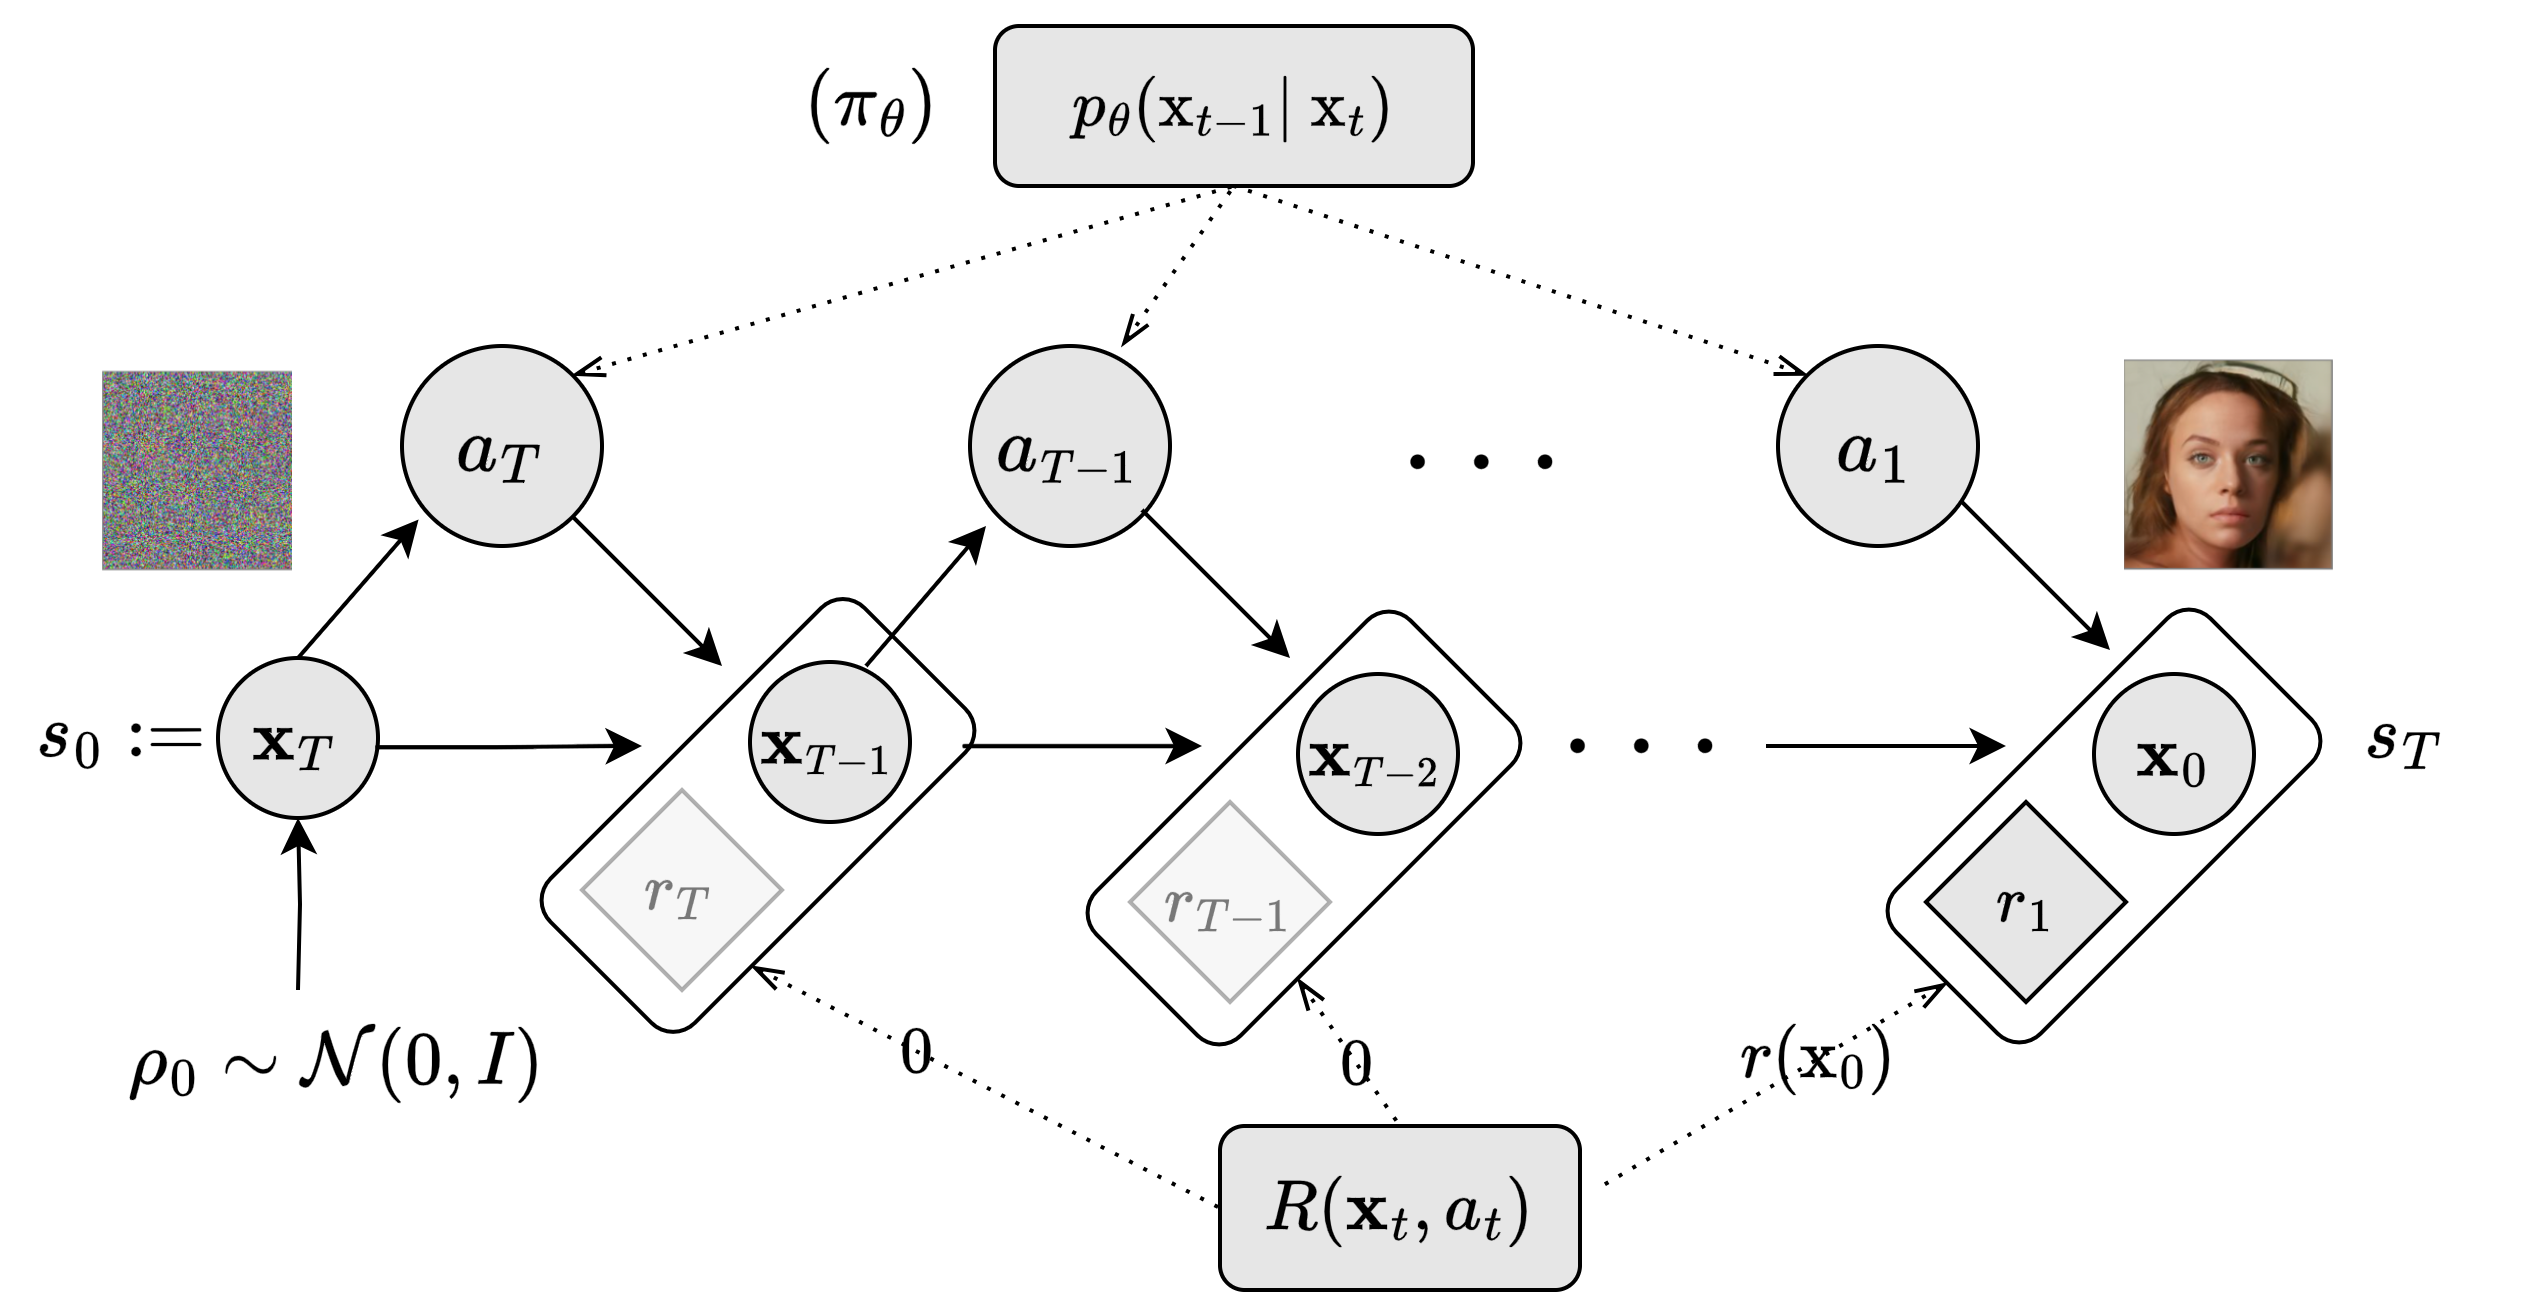
\includegraphics[scale=0.85]{img/results/diffusion-model-MDP.png}
  \vspace{-4pt}  % reduce space between caption and figure
    \captionsetup{width=\textwidth} % set the width of the caption
    \caption{\textbf{Diffusion model as a sequential decision-making process.} The policy $\pi_{\theta}:=p_{\theta}(\mathrm{x}_{t-1} | \mathrm{x}_{t})$  takes denoising decisions from pure noise to the final sample $\mathrm{x}_0$ through the entire backward process $\tau=\mathrm{x}_{T:0}$.}
  \label{fig:diffusion-model-mdp}
\end{figure}

% agregar función de reward...
We consider the \textbf{d}enoising \textbf{d}iffusion \textbf{p}olicy
\textbf{o}ptimization (DDPO) formulation \citep{black2023training} as a 
starting point. The initial state of the Markov decision process,
$\mathrm{s}_{0}$, is sampling from an isotropic Gaussian distribution 
$\rho_{0}\sim\mathcal{N}(0, I)$, corresponding to the
noise $\mathrm{x}_{T}$ at the beginning of the
diffusion backward process as shown in Figure~\ref{fig:diffusion-model-mdp},
where the sample generation starts. 
Then, a \textit{denoising} neural network $p_{\theta}$ is used to directly
estimate $\mathrm{x}_{t-1}$ at timestep $t$ (or indirectly by estimating the
noise $\hat{\epsilon}_{t}$) and is treated as a policy $\pi_{\theta}(a_{t}, s_{t})$. The policy describes how an agent---\textit{via its denoising actions $a_{t}$}---moves from a noisy
step to a less noisy one (i.e. $a_t: \mathrm{x}_{t} \rightarrow \mathrm{x}_{t-1}$) until arrives to a terminal state $s_T$, where the sample $\mathrm{x}_{0}$ is generated. \\

\noindent In this RL framework, we can optimize the diffusion
model parameters $\theta$ directly via policy gradient estimation to maximize any arbitrary scalar-reward signal over the sample $\mathrm{x}_{0}$.
In other words, the agent learns how to denoise trajectories to maximize the expected reward using the following denoising diffusion RL objective (DDRL):

% \begin{equation}\label{difusion-rl-objective-1}
%   \mathcal{J}_{\text{DDRL}}(\theta)
%   = \mathbb{E}_{\mathrm{c}\sim p(\mathrm{c}),  \mathrm{x}_{0}\sim p_{\theta}(\mathrm{x}_{0}|\mathrm{c})}[ r(\mathrm{x}_{0}, \mathrm{c})]
% \end{equation}

\begin{equation}\label{difusion-rl-objective-1}
  \mathcal{J}_{\text{DDRL}}(\theta)
  = \mathbb{E}_{\mathrm{c}\sim p(\mathrm{c}),  \mathrm{x}_{0}\sim p_{\theta}(\mathrm{x}_{0}|\mathrm{c})}[ r(\mathrm{x}_{0}, \mathrm{c})]
\end{equation}

\noindent A relevant aspect of this formulation is that the reward $R(s_{t}, a_{t})$ only provides information about the final sample $\mathrm{x}_{0}$, giving zero reward to each non-terminal state, or $\mathrm{x}_{t}$ where $t\neq0$ as it is depicted in Figure~\ref{fig:diffusion-model-mdp}. Additionally, DDPO-based methods propose two ways to compute the gradients: (i) via a score function method, denoted as $\text{DDPO}_{\text{SF}}$, also known as the REINFORCE method derived in Section~\ref{sec:reinforce}.

% agregar objetivo DDPO_{SF}
\begin{equation}\label{eqn:ddpo-sf-objective}
 (\text{DDPO}_{\text{SF}})~~ \nabla_{\theta}\mathcal{J} = \mathbb{E}_{\mathrm{x}_{T:0}\sim p_{\theta}} \bigg[\sum_{t=0}^{T}\nabla_{\theta}\log p_{\theta}(\mathrm{x_{t-1}|\mathrm{x}_t}) r(\mathrm{x}_{0})\bigg]
\end{equation}

\noindent and (ii) using importance sampling to optimize a surrogate objective \cite{schulman2015trust, schulman2017proximal}. This second approach, denoted $\text{DDPO}_{\text{IS}}$ in Equation~\eqref{eqn:ddpo-is-objective}, is more data efficient because is allowing to update a policy multiple times with the same set of trajectories collected. Therefore is used as benchmark in this work to compare the proposed method.\footnote{When we refer to DDPO from here on without specifying, it is DDPO with importance sampling (aka PPO algorithm \citep{schulman2017proximal}).} 

% agregar objetivo DDPO_{IS}
\begin{equation}\label{eqn:ddpo-is-objective}
    (\text{DDPO}_{\text{IS}})~~ \nabla_{\theta}\mathcal{J} = \mathbb{E}_{\mathrm{x}_{T:0}\sim p_{\theta_{\text{old}}}} \bigg[\sum_{t=0}^{T}\frac{p_{\theta}(\mathrm{x}_{t-1}|\mathrm{x}_{t})}{p_{\theta_{\text{old}}}(\mathrm{x}_{t-1}|\mathrm{x}_{t})}\nabla_{\theta}\log p_{\theta}(\mathrm{x_{t-1}|\mathrm{x}_t}) r(\mathrm{x}_{0})\bigg]
\end{equation}

\noindent There are some points to consider when implement Equation~\ref{eqn:ddpo-is-objective}:

\begin{enumerate}
  \item For training compatibility with automatic differentiation softwares such as PyTorch or JAX, we transform the RL objective into a loss function to minimize the negative of the objective.
  \begin{equation*}
    \begin{split}
      (\text{DDPO}_{\text{IS}})~~ \mathcal{L} = \mathbb{E}_{\mathrm{x}_{T:0}\sim p_{\theta_{\text{old}}}} \left[-\left(\sum_{t=0}^{T}\frac{p_{\theta}(\mathrm{x}_{t-1}|\mathrm{x}_{t})}{p_{\theta_{\text{old}}}(\mathrm{x}_{t-1}|\mathrm{x}_{t})} \log p_{\theta}(\mathrm{x}_{t-1}\mid\mathrm{x}_{t})\right) r(\mathrm{x}_{0}) \right]
    \end{split}
  \end{equation*}
  \item For numerical stability, the probability ratio $r_{t}$ is compute as follows:
  \begin{equation*}
    \begin{split}
      r_{t} &= \frac{p_{\theta}(\mathrm{x}_{t-1}|\mathrm{x}_{t})}{p_{\theta_{\text{old}}}(\mathrm{x}_{t-1}|\mathrm{x}_{t})} \\
      r_{t} &= \exp(\log p_{\theta}(\mathrm{x}_{t-1}|\mathrm{x}_{t}) - \log p_{\theta_{\text{old}}}(\mathrm{x}_{t-1}|\mathrm{x}_{t}))
    \end{split}
  \end{equation*}
  \item For training stability, proximal policy optimization implement the above objective by clipping the ratios and avoid large changes in the policy parameters, see Section~\ref{sec:trpo-ppo}. 
  \begin{equation*}
    \begin{split}
      (\text{DDPO}_{\text{IS}})~~ \mathcal{L} =  \mathbb{E}_{\mathrm{x}_{T:0}\sim p_{\theta_{\text{old}}}} \left[ \sum_{t=0}^{T}r_{t} \log p_{\theta}(\mathrm{x}_{t-1}\mid \mathrm{x}_{t}) A \right]
    \end{split}
  \end{equation*}
  % \item The reward is not used directly to update the policy, instead is used to compute the advantage function $A$ that is used to update the policy. 
  % The advantage function is defined as $A = R - V$, where $R$ is the reward and $V$ is the value function as explained in Section~\ref{sec:actor-critic}. However, in DDPO the value function is not used, and the advantage function is computed as a normalization of the batch rewards used to update the policy
  % parameters.
  \item Finally, it is straightforward to compute $\log p_{\theta}$ considering that $p_{\theta}$ is a conditional gaussian distribution 
  $\mathcal{N}(\mu_{\theta}(\mathrm{x}_{t})\mid\mathrm{x}_{t-1}, \alpha)$, where
  $\mu_{\theta}$ is a neural network such as U-net architecture parameterized by $\theta$. 
\end{enumerate}

% \noindent It is straightforward to compute $\log p_{\theta}$ considering that
% $p_{\theta}$ is a conditional gaussian distribution 
% $\mathcal{N}(\mu_{\theta}(\mathrm{x}_{t})\mid\mathrm{x}_{t-1}, \alpha)$, where
% $\mu_{\theta}$ is a neural network such as U-net architecture parameterized by $\theta$. %\ca{Agregar cómo despejar la formula para obtener el código?}

% \section{Extending RL in diffusion models}\label{sec:extending-methodology}

% \ca{Probablemente acá sera interesante poner ese diagrama de Venn con la intersección de modelos de difusión y RL...(?)}

% \ca{GAE y extender PPO como actor-critic usando value function es una formulación más general que DDPO. ¿Porqué no usarla? Hay unas implementaciones
% actor-critic con PPO, no creo que esto sea necesariamente GAE, pero entender
% la diferencia. Eso si, considerar siempre que la policy network se ajusta para
% y el rol del value network es mejorar la performance de la actualización de 
% gradientes. Por otro lado, la justificación de usar GAE es que se incorpora
% los reward de la trayectoria completa, lo cual es una forma de obtener tanto
% el beneficio del baseline con value function pero también de incorporar la
% información que puede tener el reward en pasos intermedios.}

% Simplifying the problem and ignoring the context raise from conditional generative models such as text-to-image, instead we assume an unconditional model free of context. Following...
% \begin{equation}\label{difusion-rl-objective-2}
%   \mathcal{J}_{\text{DDRL}}(\theta)
%   = \mathbb{E}_{\mathrm{x}_{0}\sim p_{\theta}(\mathrm{x}_{T:0})}[R(\mathrm{x}_{T:0})]
% \end{equation}

% Based on the summarization of policy gradients in \cite{schulman2015high} we can see the design decision to extend reinforcement learning, these are non excluyentes...
% \begin{equation}\label{eqn:general-pg-estimation-form}
%   \nabla_{\theta}\mathcal{J}(\theta) = \mathbb{E}\bigg[\sum_{t=0}^{\infty}\Psi_{t}\nabla_{\theta}\log\pi_{\theta}(a_{t}|s_{t}) \bigg]
% \end{equation}
% En la Figure~\ref{fig:diffusion-model-mdp}, el reward signal $\Psi_{t}$ es cero para todo $t\neq0$. Por lo tanto, el objetivo de RL se reduce a maximizar el reward en el estado terminal $\mathrm{x}_{0}$. Considering alternatives
% to extend the reward signal summarize in \textit{High-Dimensional Continuous Control Using Generalized Advantage Estimation} \cite{schulman2015high}, we propose the following formulations.

% \begin{equation}
%   g = \mathbb{E} \left[ \sum_{t=0}^{\infty} \Psi_t \nabla_\theta \log \pi_\theta (a_t | s_t) \right],
%   \end{equation}
  
%   where $\Psi_t$ may be one of the following:

%   \begin{multicols}{2}
%     \begin{enumerate}
%         \item $\sum_{t=0}^{\infty} r_t$: total reward of the trajectory.
%         \item $\sum_{t'=t}^{\infty} r_{t'}$: reward following action $a_t$.
%         \item $\sum_{t'=t}^{\infty} r_{t'} - b(s_t)$: baselined version of previous formula.
%         \item $Q^{\pi}(s_t, a_t)$: state-action value function.
%         \item $A^{\pi}(s_t, a_t)$: advantage function.
%         \item $r_t + V^{\pi}(s_{t+1}) - V^{\pi}(s_t)$: TD residual.
%     \end{enumerate}
%   \end{multicols}

%   The latter formulas use the definitions
  
%   \begin{equation}
%   V^{\pi}(s_t) := \mathbb{E}_{s_{t+1:\infty}, a_{t:\infty}} \left[ \sum_{l=0}^{\infty} r_{t+l} \right]
%   \end{equation}
  
%   \begin{equation}
%   Q^{\pi}(s_t, a_t) := \mathbb{E}_{s_{t+1:\infty}, a_{t+1:\infty}} \left[ \sum_{l=0}^{\infty} r_{t+l} \right]
%   \end{equation}
  
%   \begin{equation}
%   A^{\pi}(s_t, a_t) := Q^{\pi}(s_t, a_t) - V^{\pi}(s_t) \quad \text{(Advantage function).}
%   \end{equation}


% \ca{\textbf{Importante:} Si se encuentra implementación de GAE, todas las
% posibilidades anteriores son consideradas por este ``estimador'', por tanto,
% no sería necesario (i) consiederar cual usar o es más apropiada, (ii) 
% implementar más de una (en honor al tiempo), y (iii) considerar lo del baseline
% como una extensión aparte de considerar el reward de la trayectoria, esta
% formulación tenemos eso gratis.}

\section{Empirical Analysis on Reward Trajectory Dynamics}\label{sec:empirical-analysis}

% Reward signal during samples trajectories 
\begin{figure}[ht]
  \centering
  \begin{minipage}{0.5\textwidth}
      \centering
      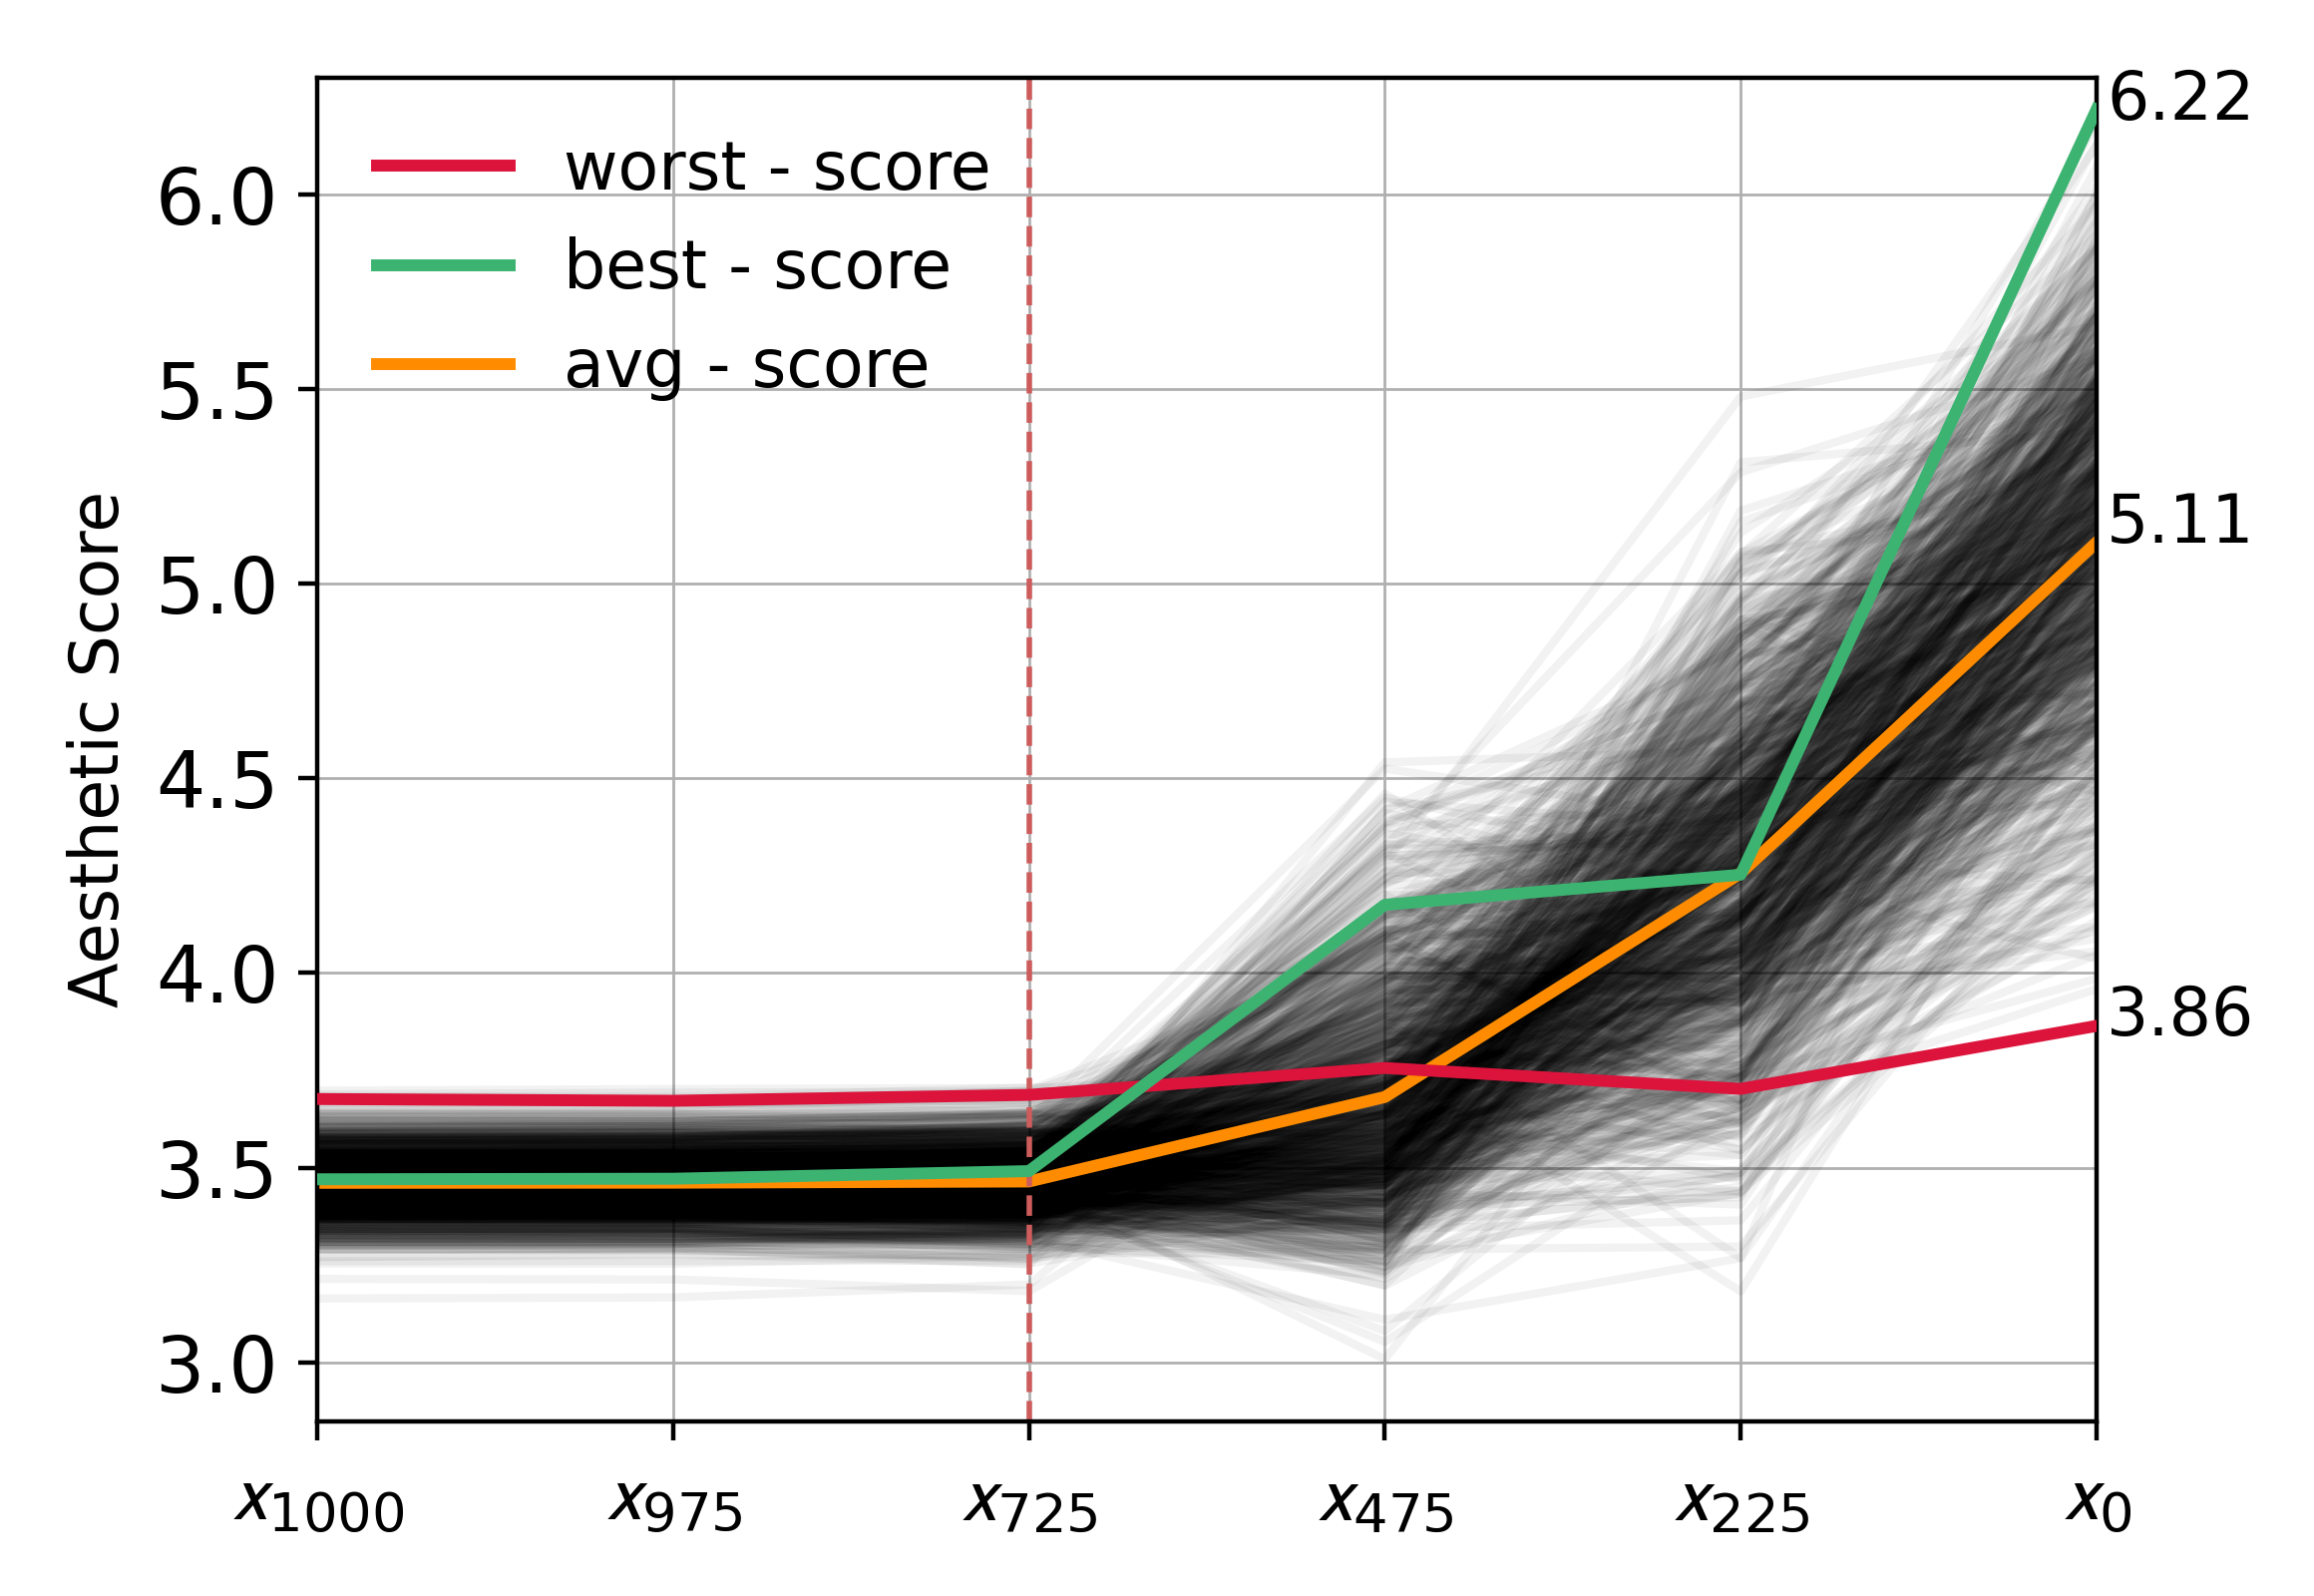
\includegraphics[width=1\textwidth]{img/results/1k-trajectories-aestheic-score-single.png} % first figure itself
  \end{minipage}\hfill
  \begin{minipage}{0.5\textwidth}
      \centering
      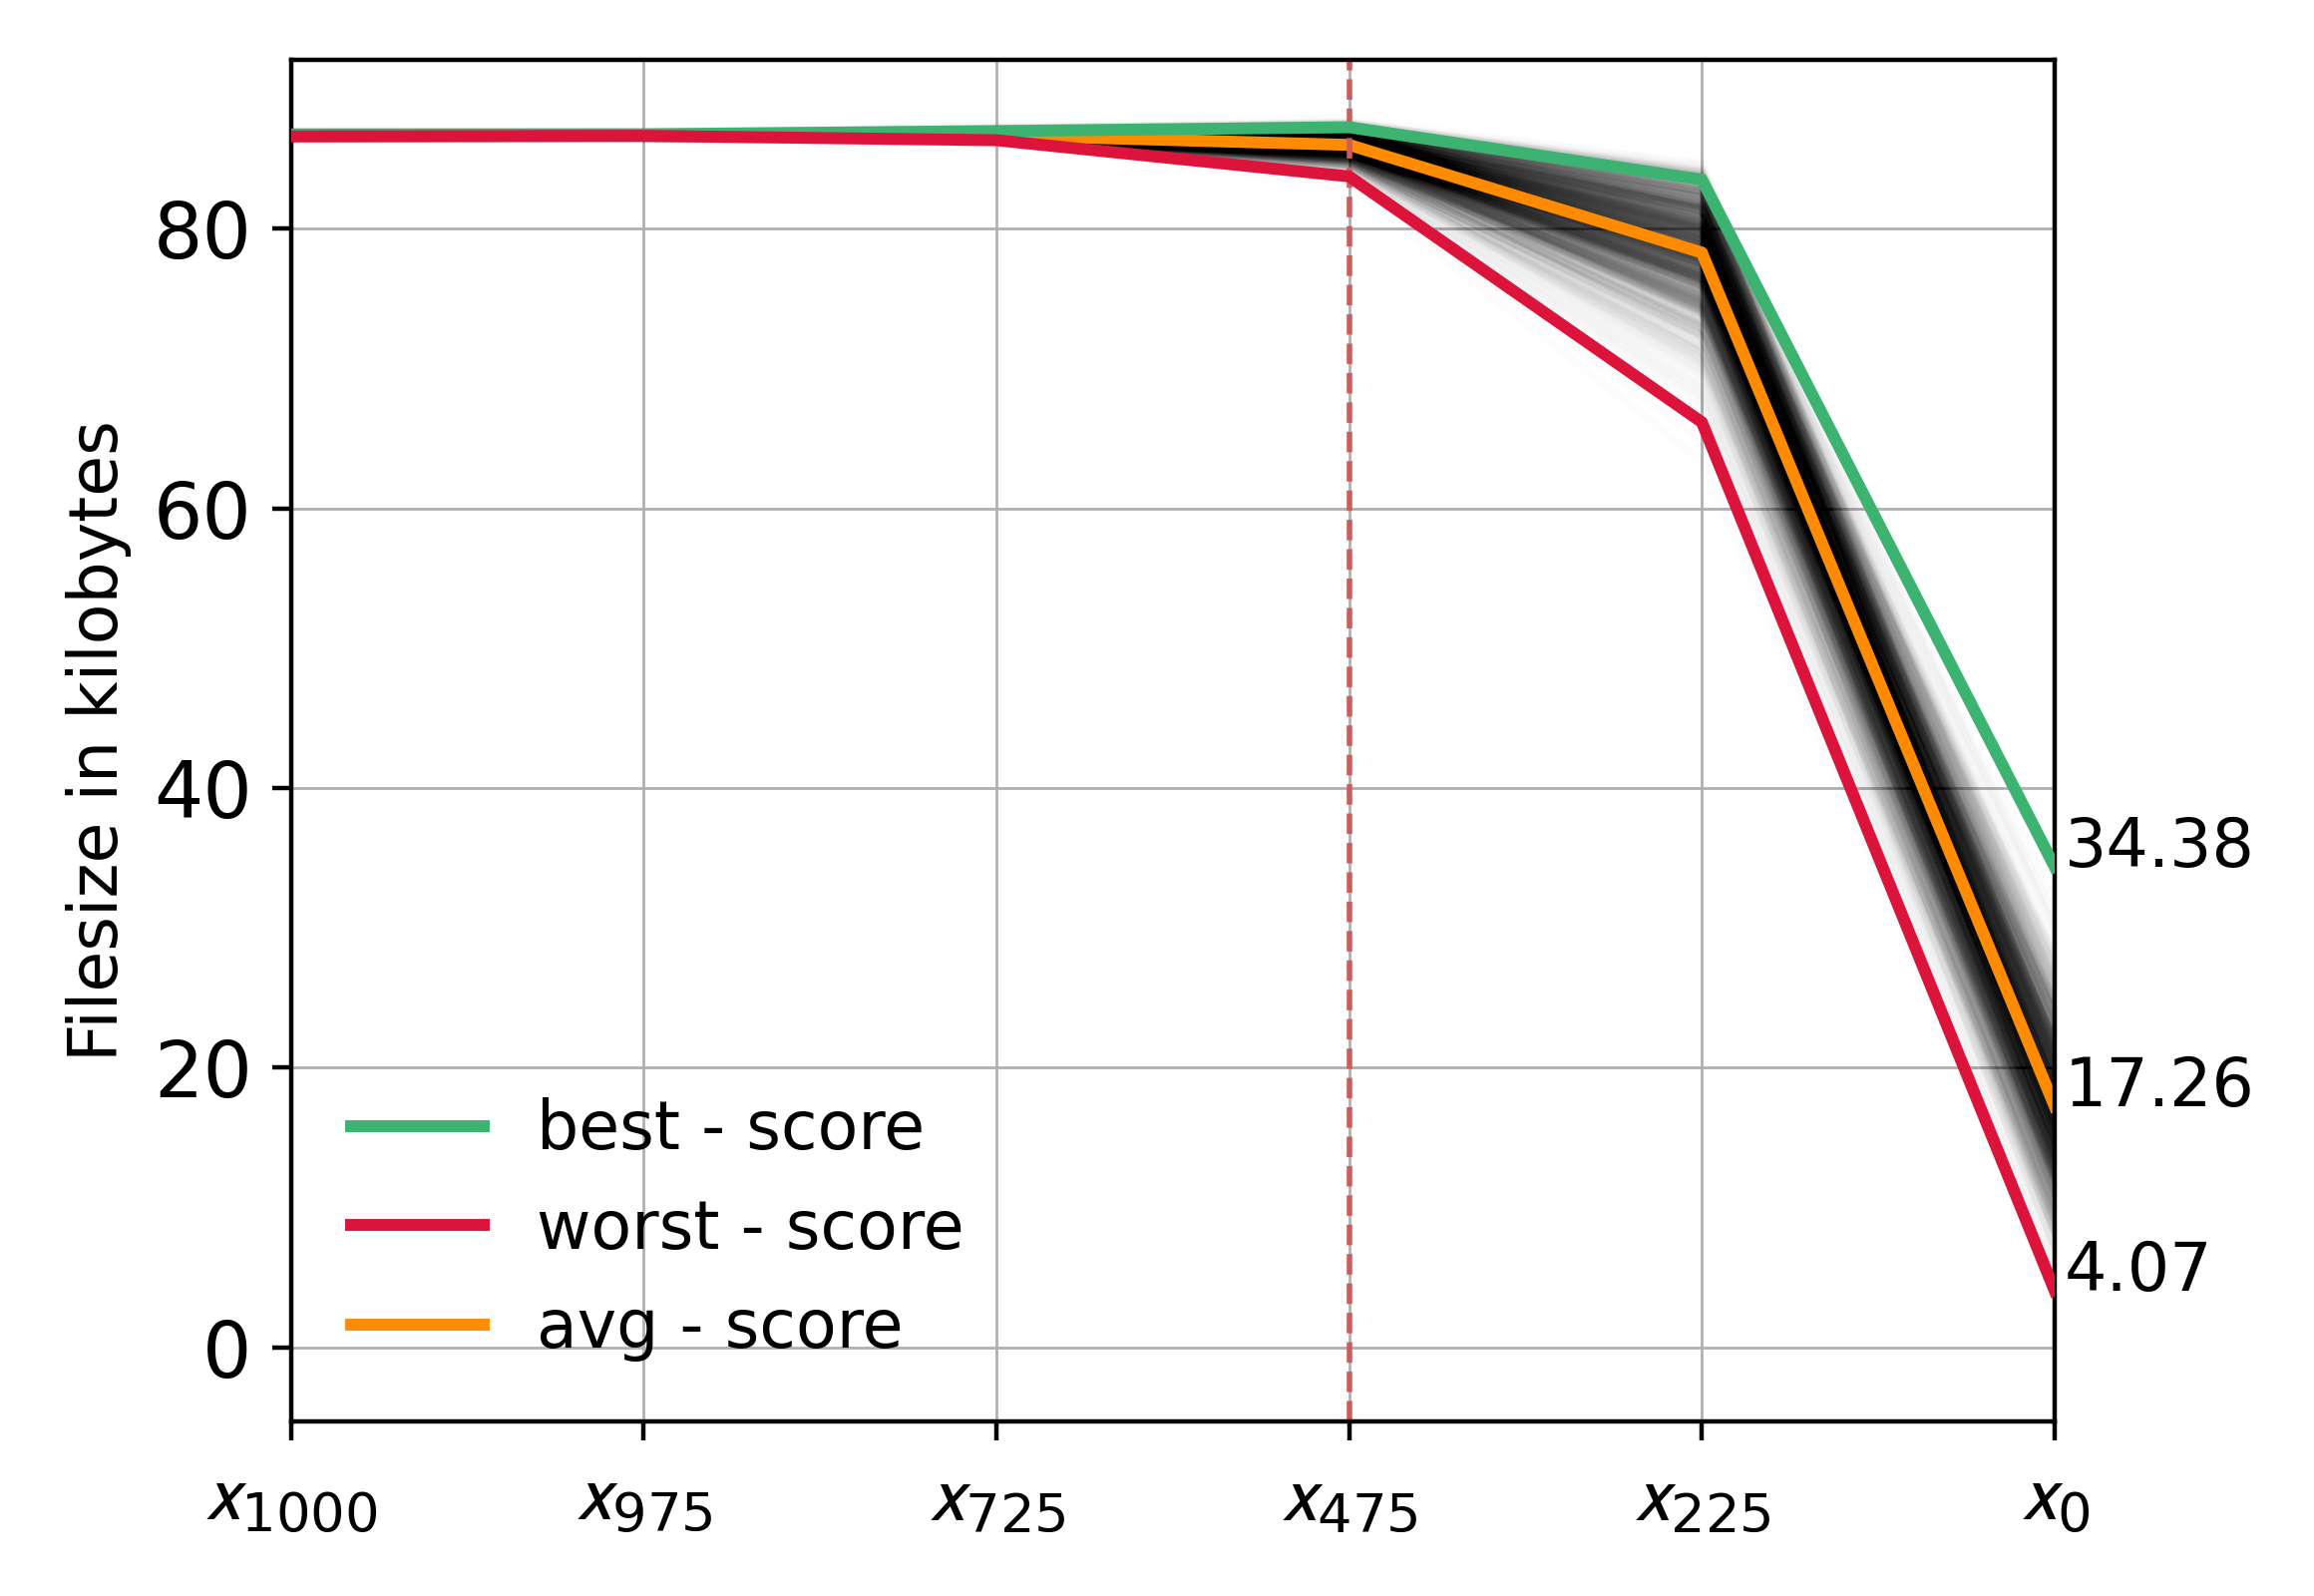
\includegraphics[width=1\textwidth]{img/results/1k-trajectories-jpeg-size-single.png} % second figure itself
  \end{minipage}\vspace{-0.1cm} % space between row 1 and row 2 of figures
  \begin{minipage}{0.5\textwidth}
      \centering
      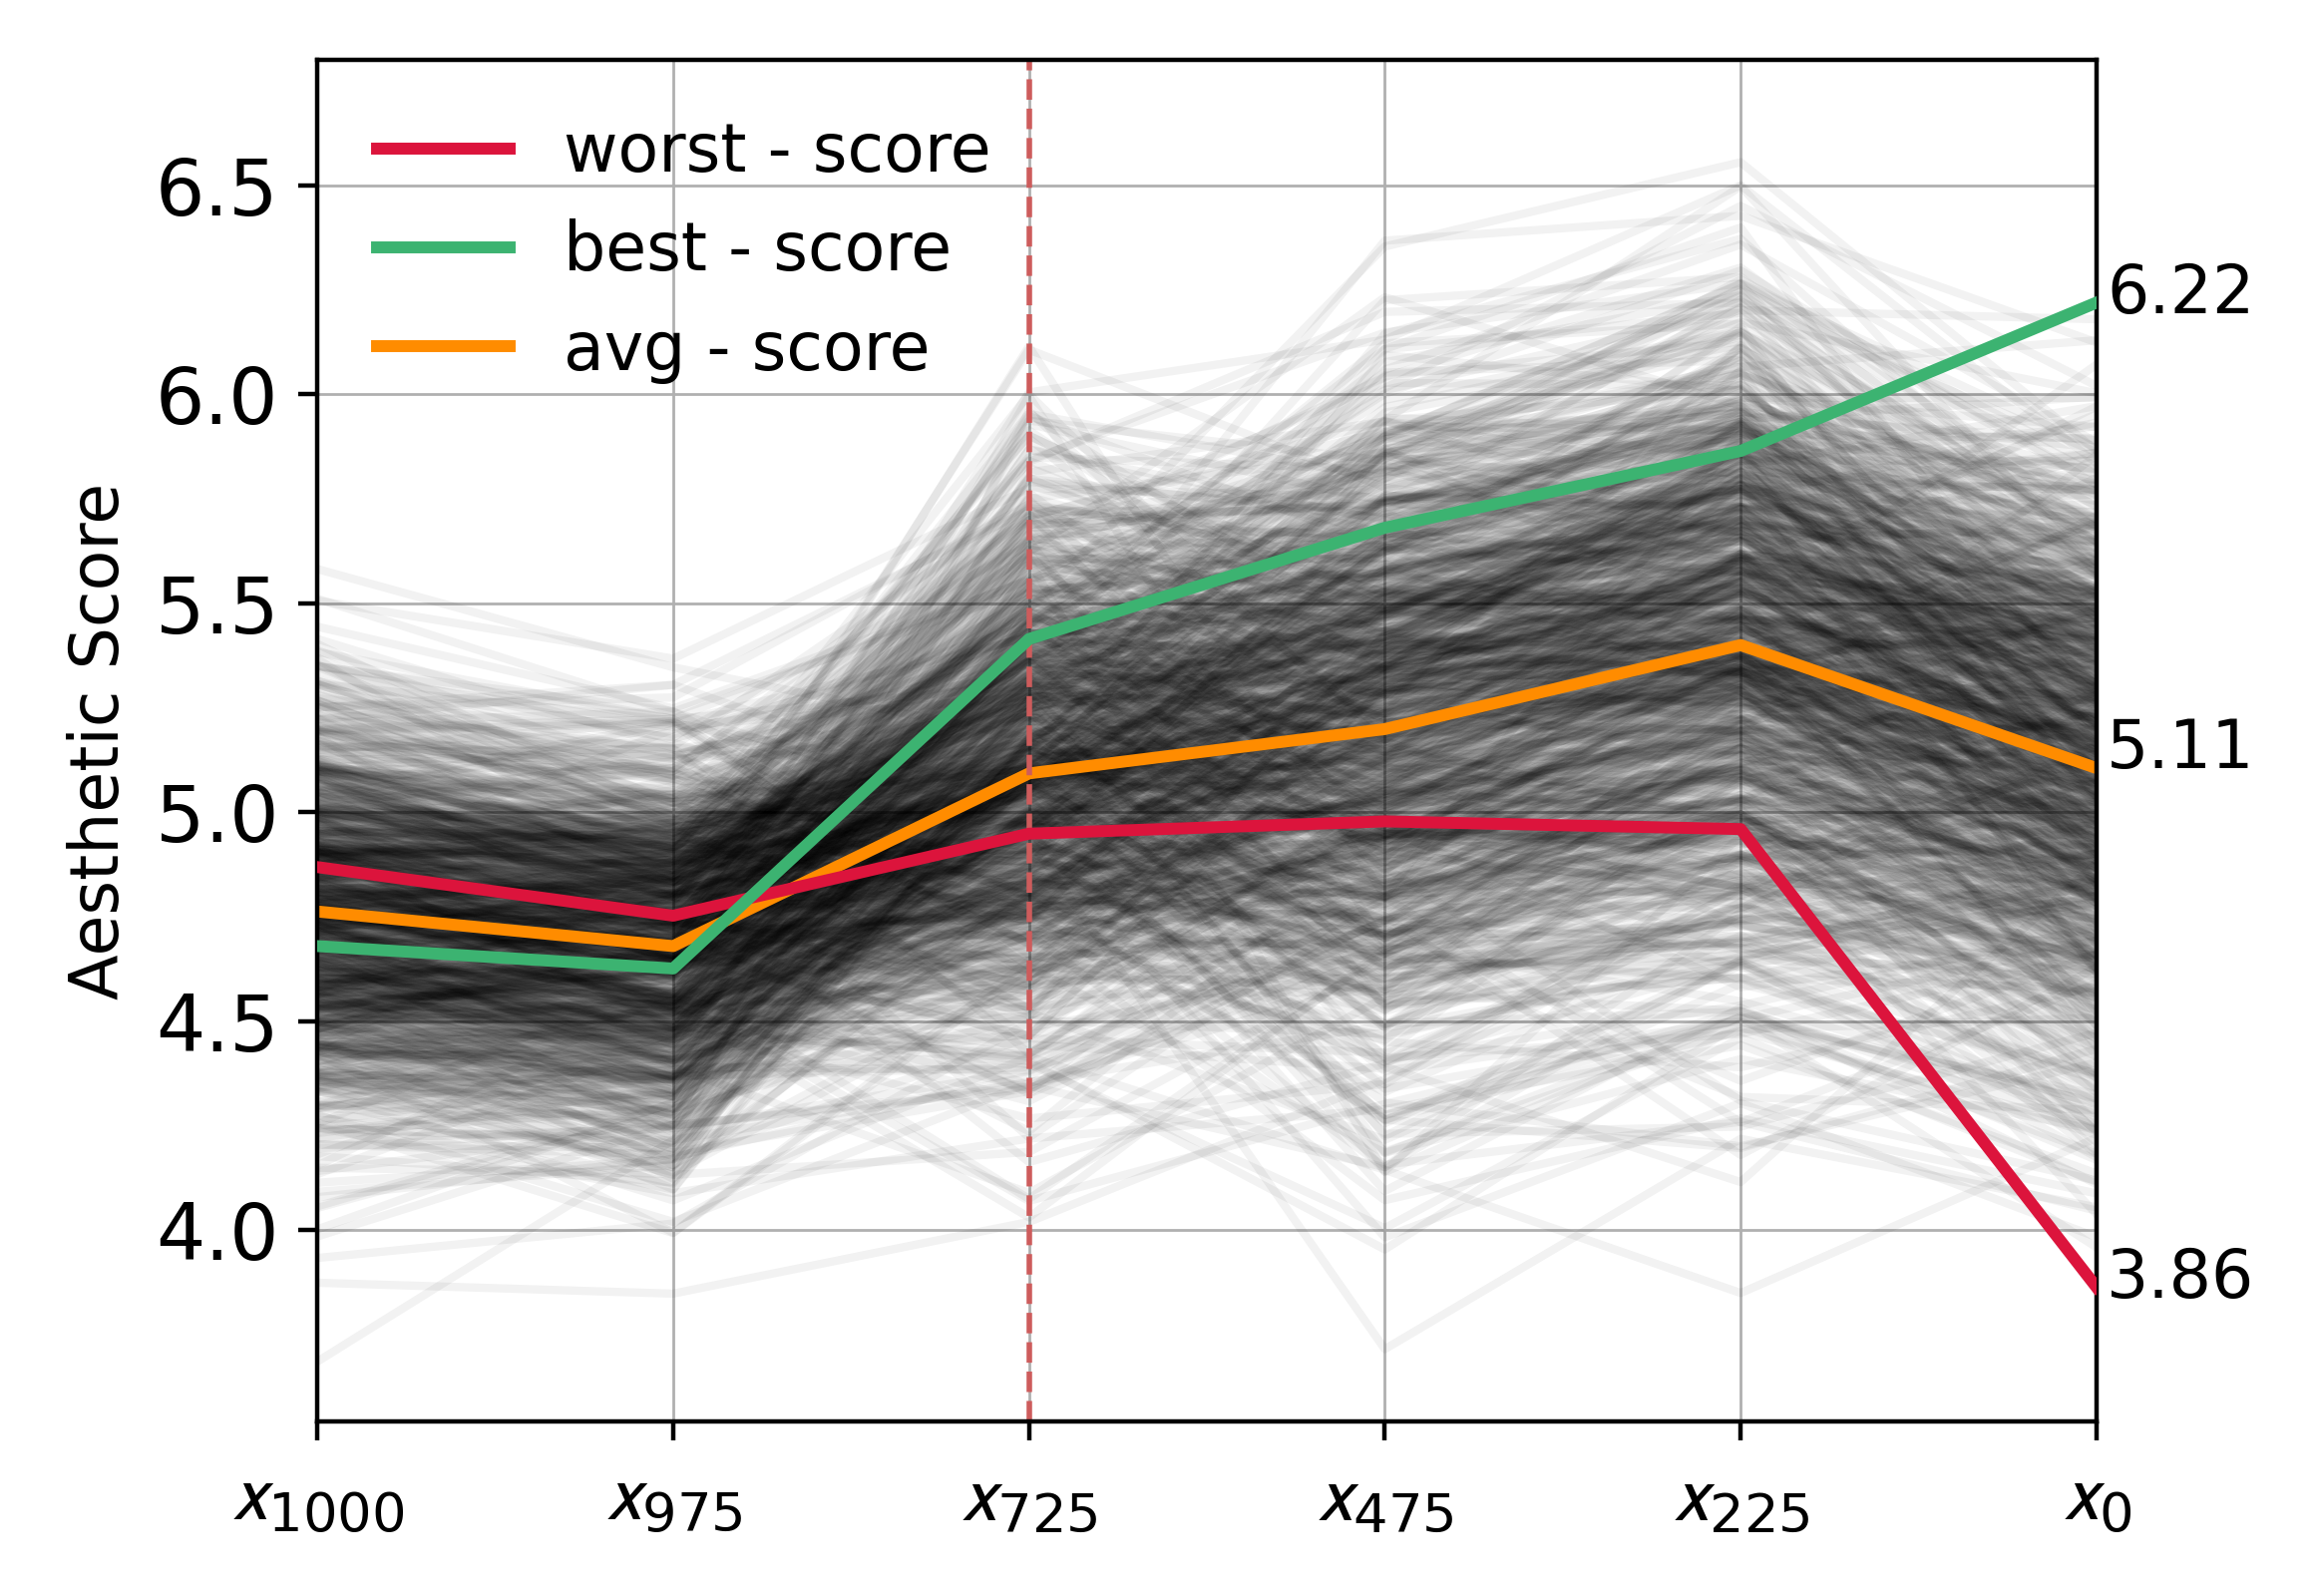
\includegraphics[width=1\textwidth]{img/results/1k-denoise-trajectories-aestheic-score-single.png} % first figure itself
  \end{minipage}\hfill
  \begin{minipage}{0.5\textwidth}
      \centering
      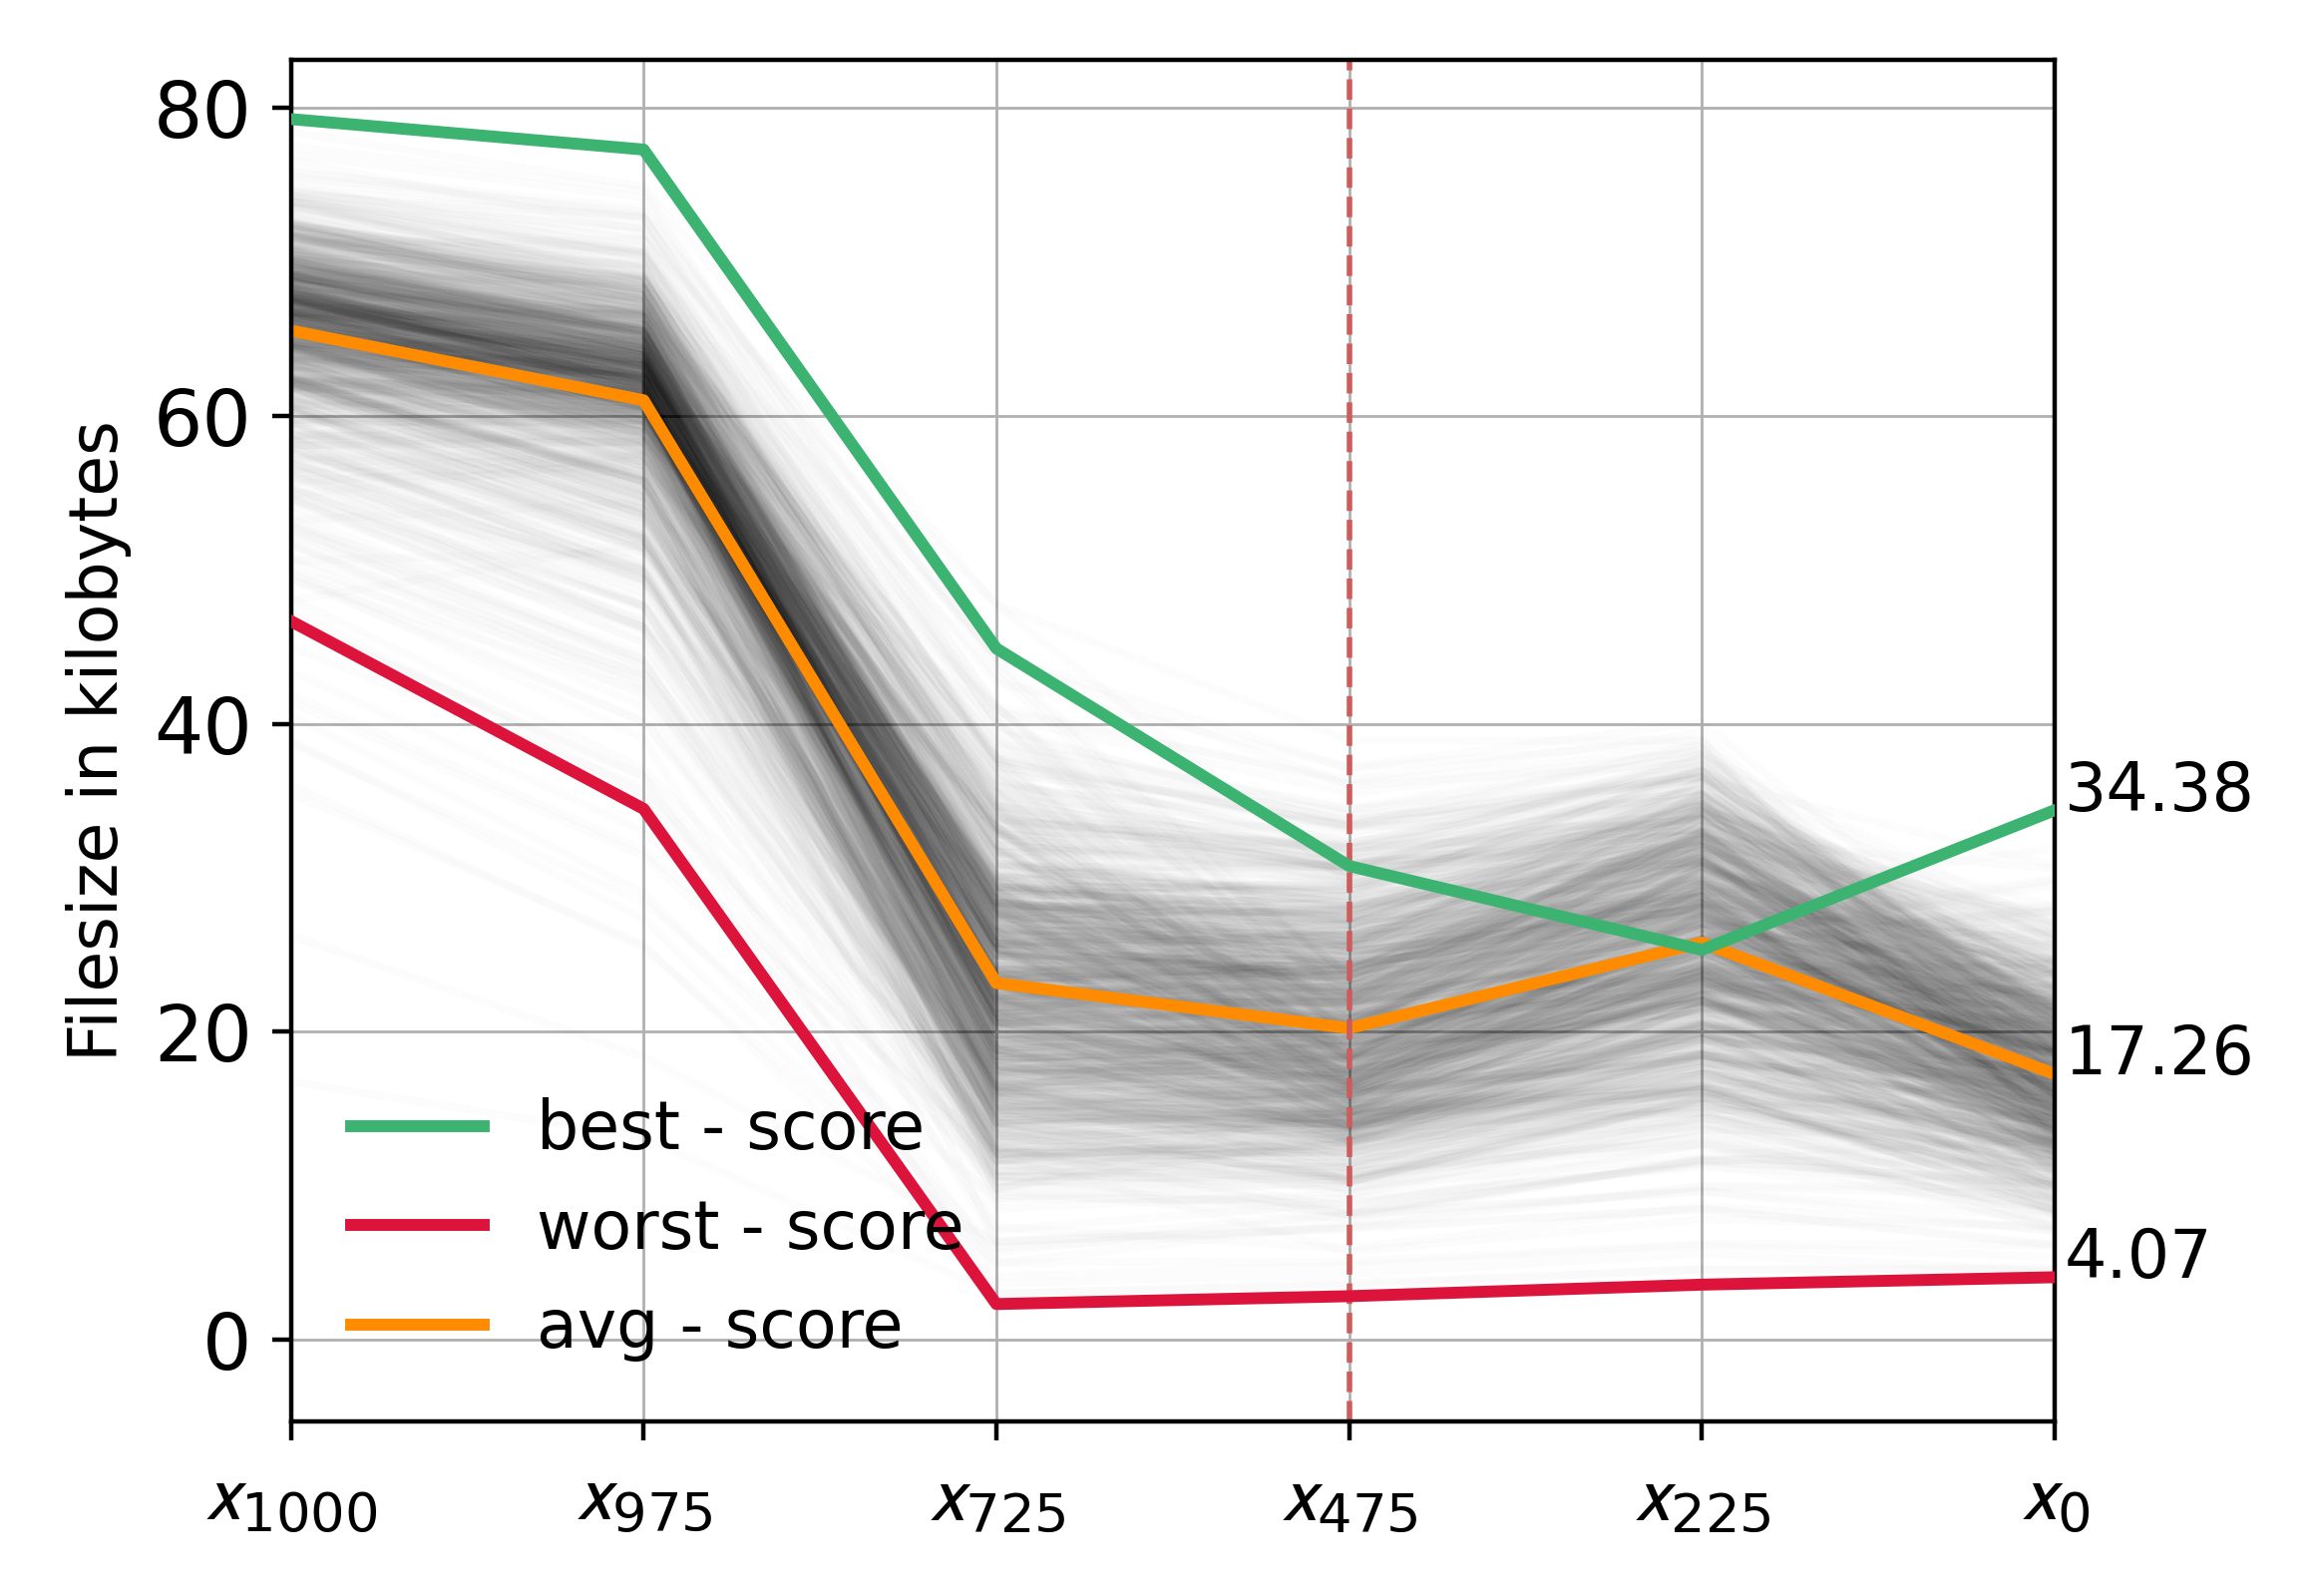
\includegraphics[width=1\textwidth]{img/results/1k-denoise-trajectories-jpeg-size-single.png} % second figure itself
  \end{minipage}
  \vspace{-8pt}  % reduce space between caption and figure
    \captionsetup{width=\textwidth} % set the width of the caption
    \caption{\textbf{Visualizing reward signal during sample trajectories.} \textbf{Left:} Evolution of the aesthetic quality as reward signal over the six states $\mathrm{x}_{\tilde{t}}$, summarizing each of the $1000$ trajectories. \textbf{Right:} Image size in kbs after JPEG compression, providing another form of reward signal for the same set of trajectories. \textbf{Top:} Rewards computed over the noisy intermediate states $\mathrm{x}_{\tilde{t}}$. \textbf{Bottom:} Rewards computed over the denoised states $\tilde{\mathrm{x}}_{\tilde{t}}$.}
  \label{fig:samples-trajectory-rewards} % Add a proper reference for the label
\end{figure}

% 1er párrafo sección de análisis empírico
\textbf{Is the reward behavior informative during sample trajectories?} 
In the previous section, we observed that DDPO relies solely on the reward from the final sample. In this section, we explore the potential of the reward signal from intermediate diffusion states, which could provide valuable insights for extending the DDPO framework to utilize the reward signal throughout the entire sample trajectory. This is crucial when applying the reward function in the context of diffusion models, as it should effectively guide the agent to maximize the reward. We present an empirical analysis of the reward signal dynamics during the sample generation process. To do so, we use the unconditional pretrained diffusion model \href{https://huggingface.co/google/ddpm-celebahq-256}{\texttt{google/ddpm-celebahq-256}} \cite{ho2020denoising}, trained on the CelebA-HQ dataset \citep{karras2017progressive}, to compile a set of trajectory samples, denoted as $\mathcal{S}_o$. \\


\noindent The $1000$ observations in $\mathcal{S}_{0}$ comprises a summary of six intermediate states extracted from each trajectory. We will sample from the model using a $40$ step subsequence $\tau$ of the diffusion chain using the \texttt{DDIMScheduler} \cite{song2020denoising}, speeding up the sampling process over the original diffusion chain of $T=1000$ steps, as we explained in section~\ref{sec:DDIM}. For computational constraint, only six intermediate state of the subsequence $\tau$ are saved, and the equivalence of this summary states $\mathrm{x}_{\tilde{t}}$ with the original DDPM steps are given in the following tuples: $(\tilde{t}=0, t=1000), (\tilde{t}=1, t=975), (\tilde{t}=2, t=725), (\tilde{t}=3, t=475), (\tilde{t}=4, t=225), (\tilde{t}=5, t=0)$. Therefore, the trajectories are describe starting from the Gaussian noise, then jumping to the step $975$, $725$, until the final sample $\mathrm{x}_{t=0}$, or $\mathrm{x}_{\tilde{t}=5}$. \\

%The reward signal for each state is obtained using the LAION aesthetic predictor and the image size after JPEG compression. The results are shown in Figure~\ref{fig:samples-trajectory-rewards}. \\

\noindent The analysis include two different reward functions. The first one is the LAION aesthetic predictor \cite{laion2022}, a multilayer perceptron (MLP) that assigns a scalar value from 1 to 10 to indicate the aesthetic quality of an image, and it was trained based on human preferences. The second reward function is the image size after JPEG compression algorithm, which is used to define two downstream tasks: compressibility and incompressibility. For compressibility, we want to maximize the negative size of the image after compression, which is equivalent to minimizing the size of the image after compression. The opposite is to maximize the size of the image after compression, which we refer to as incompressibility. The election of these reward functions were based to match the experimental pipeline use in the work that introduces DDPO \cite{black2023training}. \\

\noindent Computing the reward over each trajectory on $\mathcal{S}_{0}$ allows us to inspect the reward behavior over the sample trajectories, as shown in the top row of Figure~\ref{fig:samples-trajectory-rewards}. For the aesthetic quality (left), it is possible to observe that from the step $t=725$ ahead, the reward signal start to increase in average (orange line) and a higher variance in the reward signal is observe as the trajectory approach to the final sample $\mathrm{x}_{0}$. During approximately the first $25\%$ of the denoising process, the signal is concentrate with minor variation between a $3.5$ aesthetic score. That is close to the aesthetic score that we obtain when we apply the LAION aesthetic predictor to a purely gaussian random noise. At the end, we achieve a $5.11$ average (orange line) aesthetic score, a $6.22$ and $3.86$ corresponding to the best (green line) and worst (red line) aesthetic score. \\

\noindent For the image size after JPEG compression (right), the reward signal is more stable over the trajectory, and the variance is lower than the aesthetic quality reward signal. The average image size of the final samples after JPEG compression is $17.26$ kilobytes (orange line), and the best (green line) and worst (red line) filesizes are $34.38$ and $4.07$ kilobytes, respectively. The results show that the reward signal start to be some informative on intermediate states from the step $t=475$ ahead, but with a lower variance than the aesthetic quality reward signal. The reason is that the noise is difficult to compress, and the JPEG compression can start to have effects on the image size reduction when the semantic of the image start to appear and the entropy is reduce.  \\

\noindent The top row of Figure~\ref{fig:samples-trajectory-rewards} shows the rewards computed directly over the intermediate states, i.e. structure plus noise. However, there is an issue in doing this, and could be the reason of why is a good idea to only compute the reward on the final samples $\mathrm{x}_{0}$, as is illustated in the Markov
Decision Process (MDP) formulation for a diffusion a model in Figure~\ref{fig:diffusion-model-mdp}. The reward function to control the model is design to maximize the reward in the final sample, which is a state that can be directly guide by the human preferences. Of course that we can 
provide human preferences between noisy states, but nothing guarantee that
the denoising trajectories will be consistent in the following states. Similar with the JPEG compression, the goal is to generate images of lower size, and
this endeavour it has nothing to do with the noise involved in the sample generation process. Therefore, we have a communicational gap between the intermediate states and the reward signal, a similar problem that occur using
classifier guidance with a model that is not robust to the noise to guide
the generative process \cite{bansal2023universal}. \\

\noindent \noindent \textbf{Denoised sample trajectories.} We will use the denoised observations $\tilde{\mathrm{x}}_{t\rightarrow 0}$ for the initial
noise and each intermediate step $t$ of the sample trajectories, as referred in the DDIM section~\ref{sec:DDIM}:
\begin{equation}\label{eqn:ddim-predicted-sample}
  \tilde{\mathrm{x}}_{t\rightarrow0}=f_{\theta}^{(t)}=\frac{\mathrm{x}_{t}-\sqrt{1-\alpha_{t}}\epsilon_{\theta}^{(t)}(\mathrm{x}_{t})}{\sqrt{\alpha_{t}}}
\end{equation}

\noindent As you can see in Figure~\ref{fig:sample-trajectories}, the denoised samples $\tilde{\mathrm{x}}_{t\rightarrow0}$ are fairly similar to the
final sample. The denoised intermediate state $\tilde{\mathrm{x}}_{725\rightarrow0}$ almost captures the essence of the final sample $\mathrm{x}_{0}$, and $\tilde{\mathrm{x}}_{1000\rightarrow0}$ is a highly informative latent encode of the high level features such image pose, gender, hair style and colors of the final image. Notice that in the same point in Figure~\ref{fig:samples-trajectory-rewards} (bottom-left), we have an increasing dispersion in the aesthetic score trajectory distribution from the start. This is a clear indication that the reward signal is more informative in the denoised samples than in the noisy samples. The same behavior is observed for the image size after JPEG compression (bottom-right), where the variance is higher in the denoised samples than in the noisy samples. That is because the
JPEG compression knows in advance which trajectories contain features that can be compressed or not.

% Trayectorias resumidas de google/ddpm-celebahq-256 usando DDIM scheduler y con
% los estados intermedios denoised usando formula DDIM. Se reportan los reward
% de cada imagen...
\begin{figure}[ht]
  \centering
  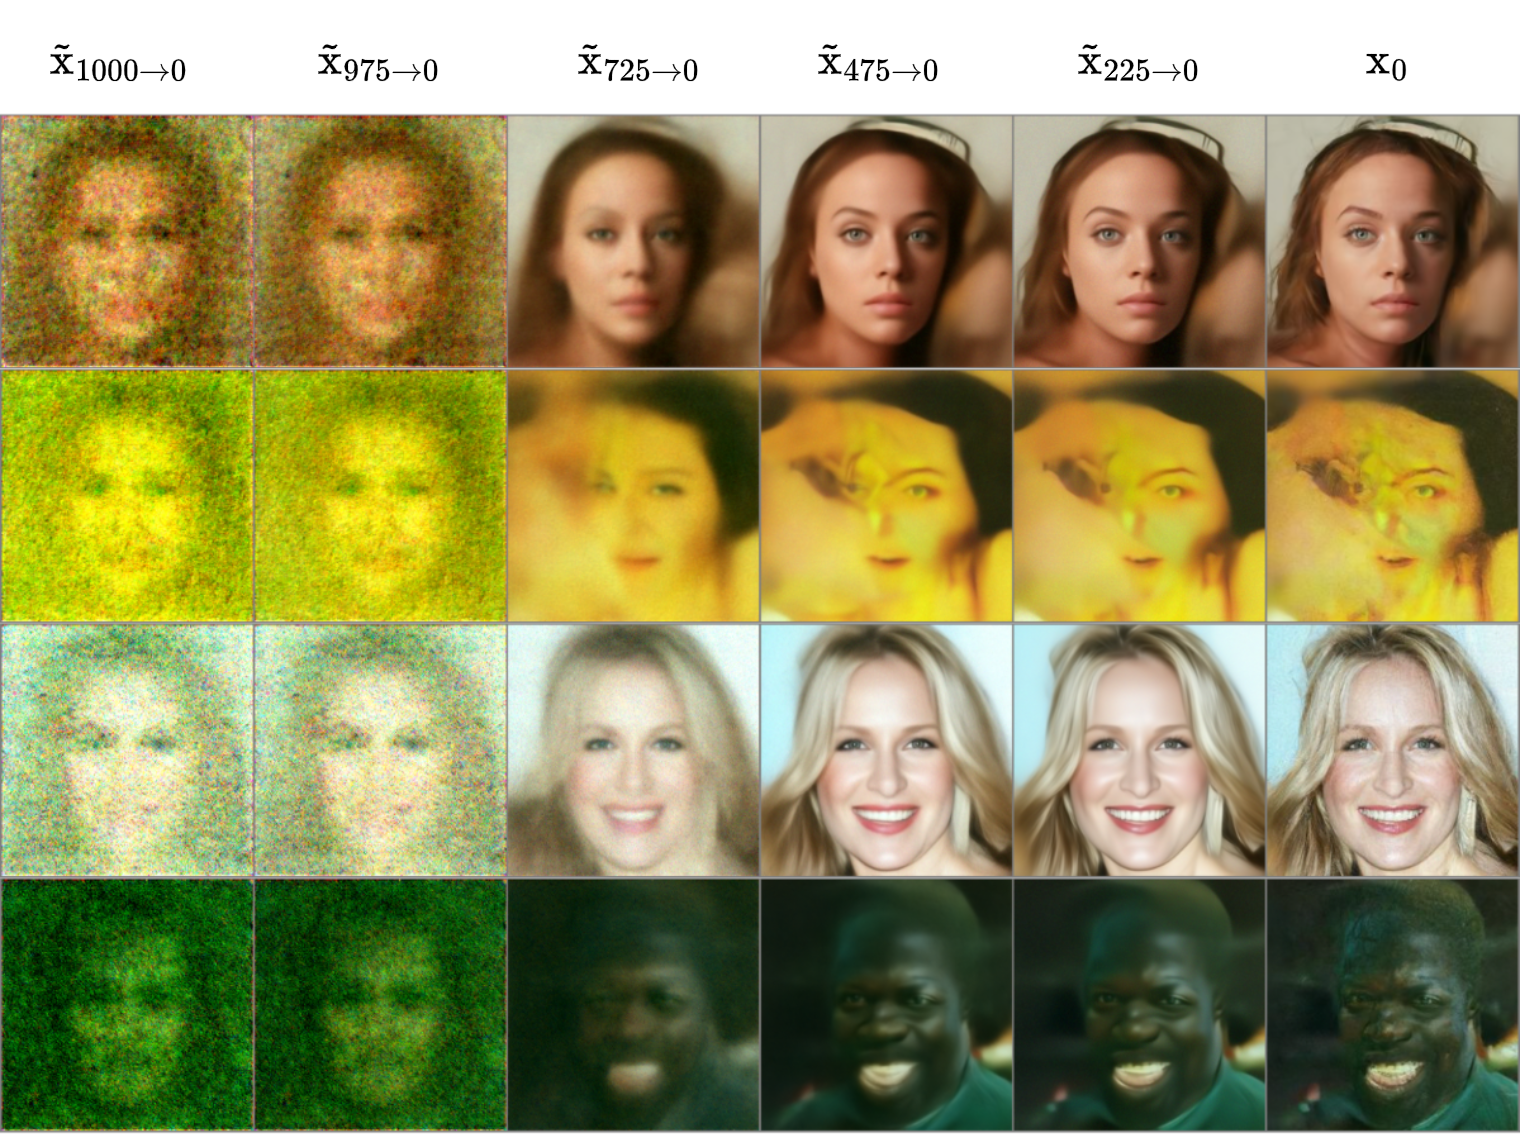
\includegraphics[scale=0.85]{img/results/denoised-samples-trajectories.png}
  \vspace{-5pt}  % reduce space between caption and figure
    \captionsetup{width=\textwidth} % set the width of the caption
    \caption{\textbf{Denoised sample trajectories.} Each row, from \textbf{top-to-bottom}, represents the best ($6.22$)
  and worst ($3.86$) aesthetic scores, and the highest ($34.38$) and lowest 
  ($4.07$) filesizes in kilobytes after JPEG compression for the final samples
  $\mathrm{x}_{0}$ in $\mathcal{S}_{o}$. Each column, from \textbf{left-to-right}, summarizes the states for each denoised sample's trajectory using Equation~\ref{eqn:ddim-predicted-sample}. The rows correspond to the trajectories highlighted in the green and red lines of Figure~\ref{fig:samples-trajectory-rewards}.}
   \label{fig:sample-trajectories}
\end{figure}


\section{Experiments}

We aim to reproduce the implementation outlined in \textit{``Training Diffusion Models with Reinforcement Learning''} \cite{black2023training} within a more streamlined setting to facilitate experimentation, while still capturing the complexity of text-to-image models for experimenting with reward functions.
Our baseline will be the generative capabilities of the pretrained \href{https://huggingface.co/google/ddpm-celebahq-256}{\texttt{\texttt{google/ddpm-celebahq-256}}} model, as described in DDPM section \cite{ho2020denoising}. This is an unconditional model that generates $256\times256$ pixel RGB images of human faces, and it operates in pixel space, predating latent diffusion models \cite{rombach2022highresolution}, so the denoising process occurs in the pixel space. \\


% Se habla sobre la metodología usada para evaluar...
\noindent \textbf{Evaluation Dataset.} We use the final samples of each trajectory in $\mathcal{S}_{0}$---\textit{described in section \ref{sec:empirical-analysis}}---as a baseline for assessing the generative performance of the pretrained model on downstream tasks. In the following sections, we evaluate the experiments using the same seeds to generate samples with finetuned checkpoints, and report the mean and standard error of the rewards across the evaluation samples. These metrics serve as the quantitative evaluation criteria in this work, enabling us to compare the performance of the finetuned models against the pretrained one. \\


\noindent To strengthen the evaluation, a visual comparison is presented between samples generated by the pretrained model and those produced by the finetuned models using identical initial noise. This comparison allows for a qualitative analysis of the changes in samples resulting from the finetuning process. Figure~\ref{fig:visual-comparison-ddpo} illustrates this visual comparison, with additional samples using the same initial noise provided in Appendix~\ref{appendix:additional-celebahq-samples}. The batches of $100$ images are arranged in the same order to ensure direct comparability. Furthermore, studying the transition from the pretrained model to the final model optimized by the reward function is essential. For this purpose, several figures depict the transition, highlighting the changes in the samples throughout the process. \\


\subsection{Reproducing DDPO}

\noindent In our experiments, we employed three downstream tasks as outlined in (Black, 2023 \cite{black2023training}): compressibility, incompressibility, and aesthetic quality. The first two tasks are defined by the size of images after applying a JPEG compression algorithm, serving as the reward function. For aesthetic quality, we utilized the LAION aesthetic model \citep{laion2022}, a multilayer perceptron that assigns a scalar value from 1 to 10 to indicate the aesthetic quality of an image. \\

\noindent These tasks effectively demonstrate the flexibility of using reinforcement learning to learn new downstream objectives. Supervised learning finetuning often struggles to encode tasks like compressibility and incompressibility into a loss function, whereas RL can optimize these tasks directly through a reward function. Additionally, the LAION aesthetic model, trained on human preferences, exemplifies how human feedback can be incorporated to align sample generation with desired outcomes. This is a key advantage of using RL with generative models \cite{ouyang2022training}. \\

\noindent Using the size of the image after JPEG compression as reward function, we can define two downstream tasks: \textit{compressibility} and \textit{incompressibility}. For compressibility, we want to maximize the negative size of the image after compression. This is equivalent to minimizing the size of the image after compression. The opposite is to maximize the size of the image after compression, which we refer to as incompressibility. \\


\subsection{Experiment results}

In Table~\ref{tab:reward-results} we have a summary of the results for each downstream tasks. The baseline are the initial performance of the pretrained DDPM model. The results show that the DDPO fintuned models outperform the baseline in all tasks, regarding the mean reward over the evaluation samples. A set of images generated under the same initial noise by the pretrained model and the finetuned models are provided for a quality comparison in Figure~\ref{fig:visual-comparison-ddpo}. In most cases, the general semantic of faces mantain---\textit{still identifying the same subject what
is depicted in the original sample}---while DDPO induce modification at high level features to achieve the reward objective. Additional comparative samples in the Appendix~\ref{appendix:additional-celebahq-samples}. \\

% \textbf{Downstream Task} & \textbf{Baseline} & \textbf{DDPO} & \textbf{I-DDPO}\\
\begin{table}
\centering
\begin{tabular}{lcc}
\toprule
\textbf{Downstream Task} & \textbf{Baseline} & \textbf{DDPO} \\
\midrule
\textbf{\texttt{google/ddpm-celebahq-256}} & & \\
\quad Aesthetic Score (higher is better) & 5.11 $~\pm$ 0.01 & \textbf{5.58} $~\pm$ 0.01 \\
\quad Compressibility (lower is better) & 17.26 $~\pm$  0.15 & \textbf{6.01} $~\pm$ 0.13 \\
\quad Incompressibility (higher is better) & 17.26 $~\pm$ 0.15 & \textbf{21.6} $~\pm$ 0.12 \\
\quad Over 50 years old (higher is better) & -7.72 $~\pm$ 0.17 & \textbf{7.39} $~\pm$ 0.16 \\
\hline
\textbf{\texttt{google/ddpm-church-256}} & & \\
\quad Aesthetic Score (higher is better) & 4.77 $~\pm$ 0.01 & \textbf{5.13} $~\pm$ 0.01  \\
\quad Compressibility (lower is better) & 29.57 $~\pm$  0.29 & \textbf{10.62} $~\pm$ 0.18  \\
\quad Incompressibility (higher is better) & 29.57 $~\pm$ 0.29 & \textbf{50.21} $~\pm$ 0.34  \\
\bottomrule
\end{tabular}
\captionsetup{width=\textwidth} % set the width of the caption
\caption{\textbf{Mean and standard error for each downstream task across two pretrained models}. All samples were generated using the same initial noise to ensure a fair comparison. \textbf{Baseline} refers to the generative capabilities of the pretrained model, as represented by $\mathcal{S}_{0}$ (see Section~\ref{sec:empirical-analysis}). \textbf{DDPO} displays results from the finetuned models using DDPO with importance sampling (see Section~\ref{sec:diffusion-model-mdp}).}
\label{tab:reward-results}
\end{table}

% \noindent Optimizing for the image size of the samples. The fintuned can be achieved using a fixed learning rate ($1e-5$), resulting in smooth transitions in the image as the model parameters shift from the initial  pretrained DDPM model to the final DDPO finetuned model. This process is  illustrated in Figure~\ref{fig:ddpm-to-ddpo-compressibility} and Figure~\ref{fig:ddpm-to-ddpo-incompressibility} for each respective reward. \\

\noindent \textbf{Emergent effects in face generation using JPEG Compressibility as reward.} Certain effects emerge as the entropy of the images is reduced, allowing for greater compression and reduced file size. Some of the recurring effects during the adjustment process include the elimination of details such as hair definition, reduction in lighting, simplification of image backgrounds, appearance and intensification of shadows, increased intensity around the contours of the eyes, and enhanced facial depth, among others. \\

% Effects of JPEG compressibility
\begin{figure}[ht]
  \centering
  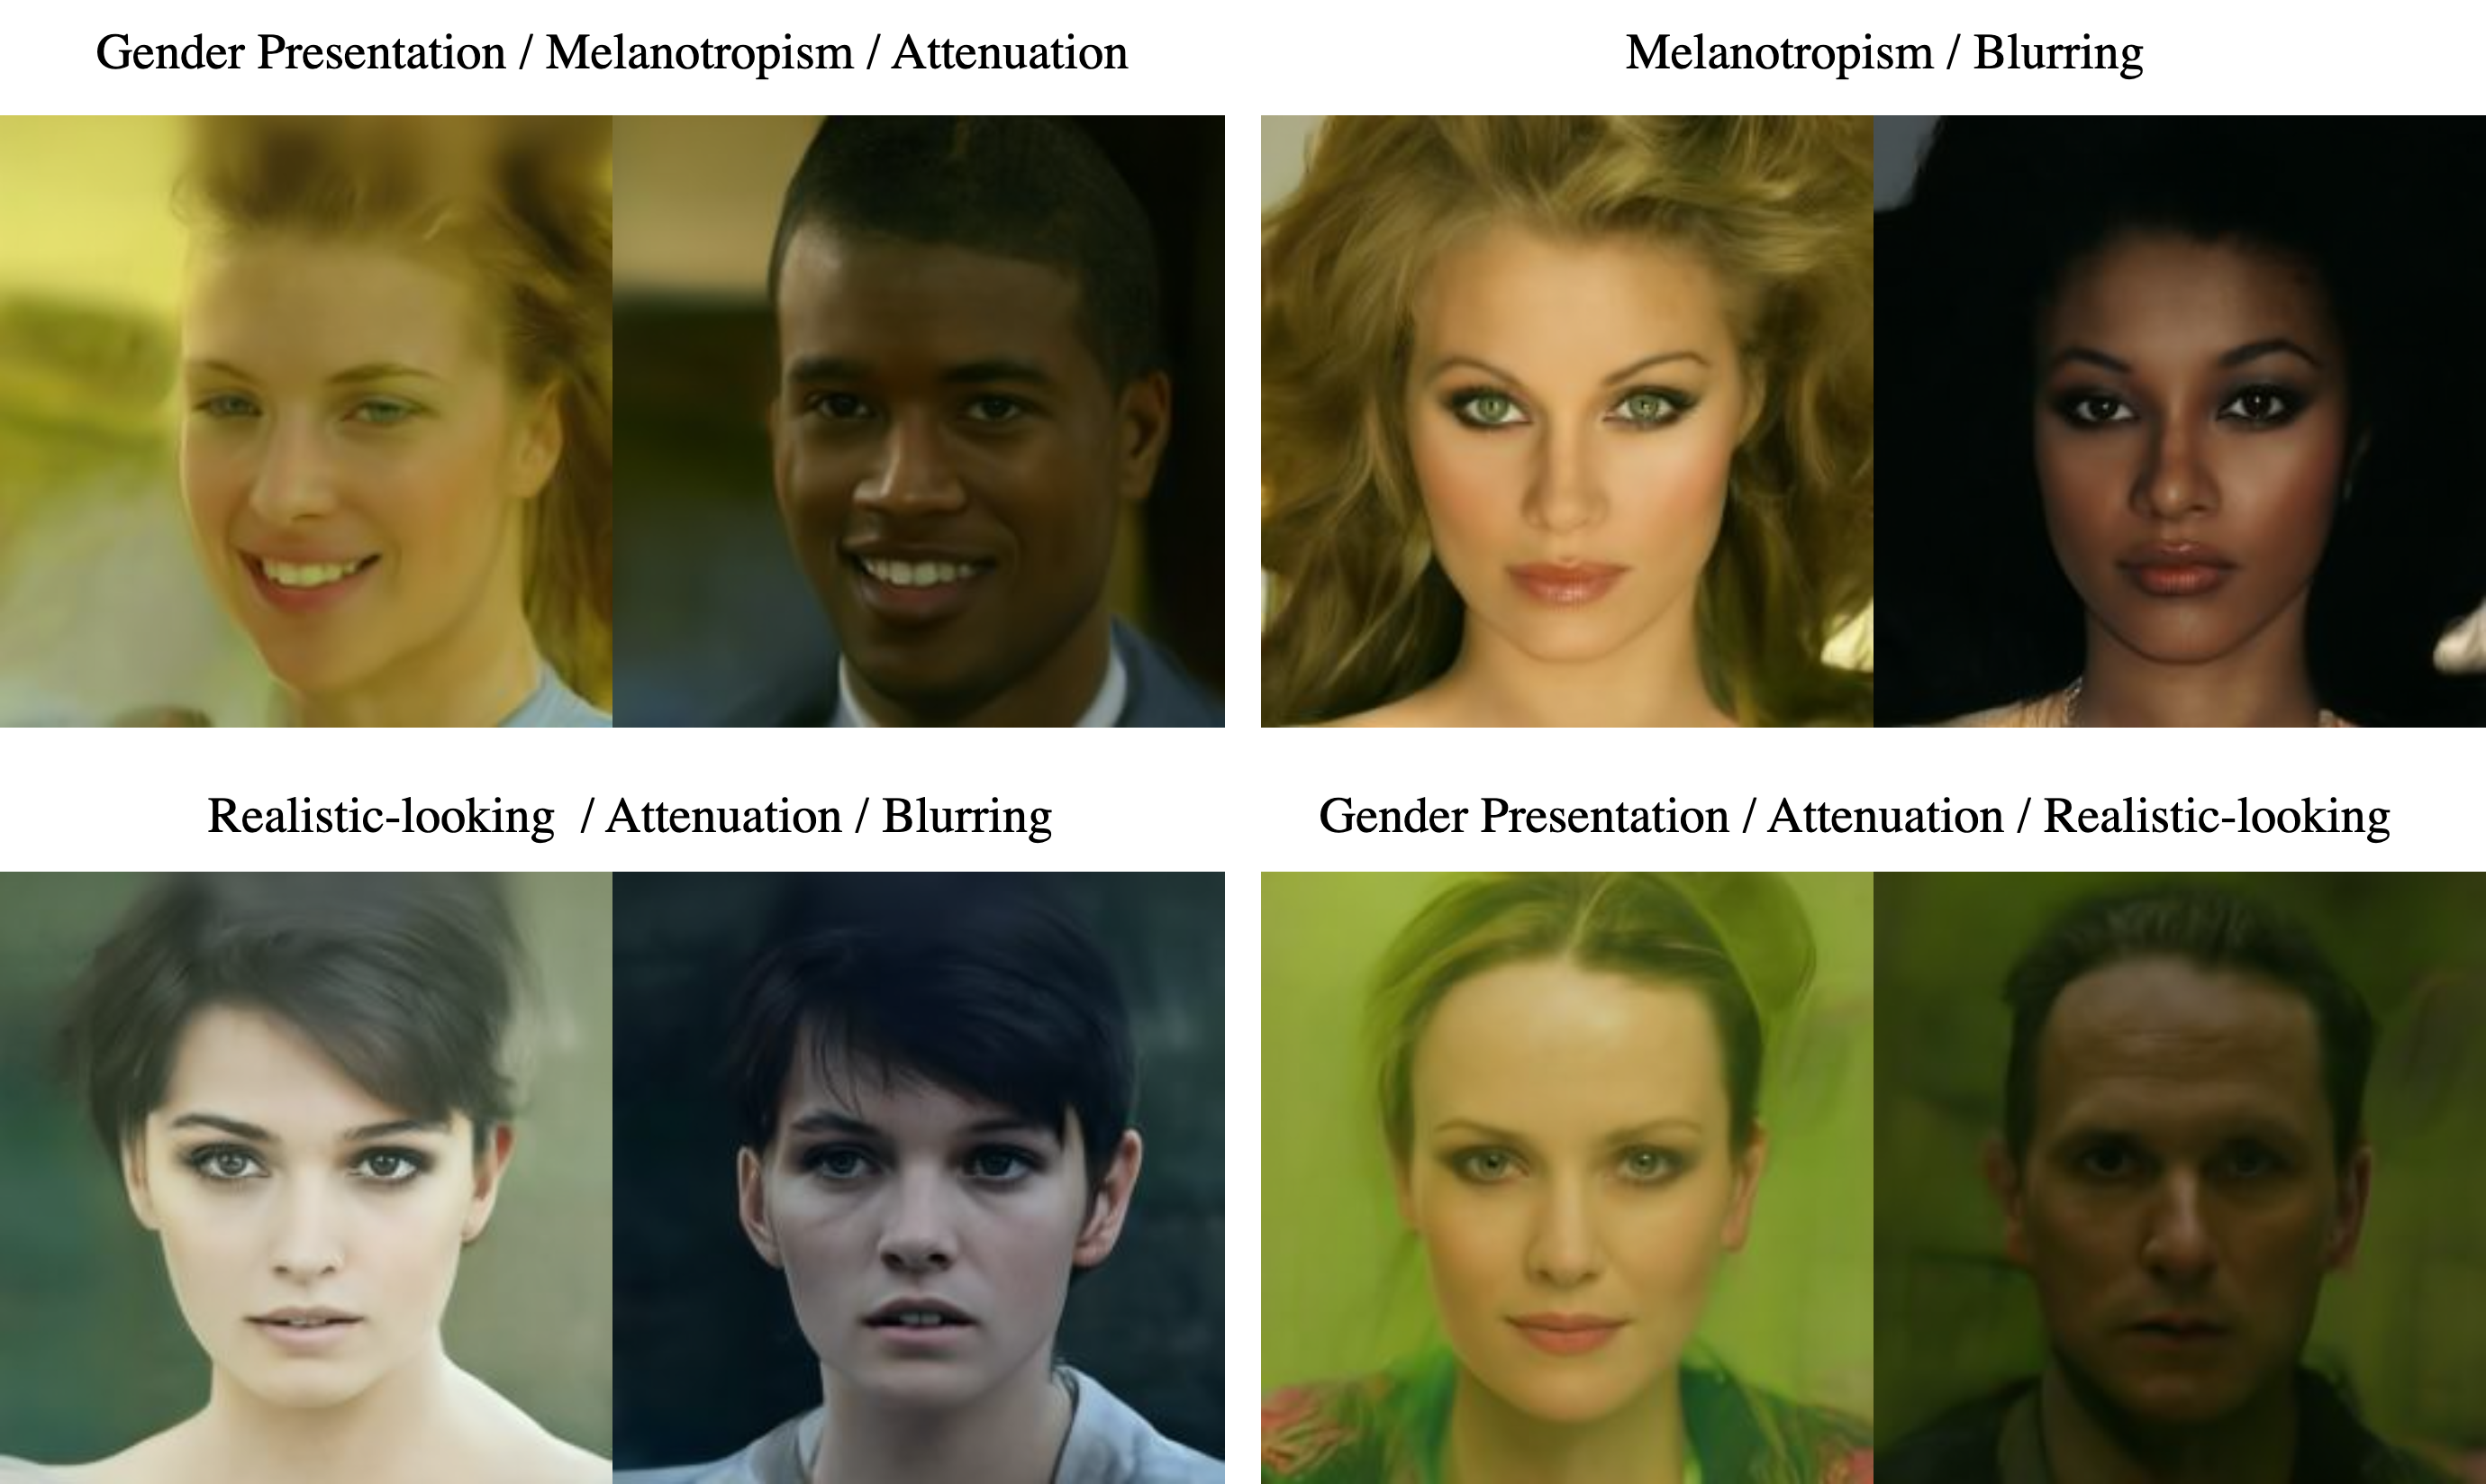
\includegraphics[scale=0.85]{img/results/compressibility-effects.png}
  \vspace{-0pt}  % reduce space between caption and figure
    \captionsetup{width=\textwidth} % set the width of the caption
    \caption{\textbf{Emergent effects in face generation using JPEG Compressibility as reward.} The top row shows increased darker skin tones (melanotropism), while the bottom row displays more realistic facial expressions. Diagonal images illustrate gender presentation phenomenon due to hair detail loss and shading effects.}
    \label{fig:compressibility-effects}
\end{figure}

\noindent In Figure~\ref{fig:compressibility-effects}, images generated by the pretrained model are compared to those generated by the finetuned model with DDPO to maximize compressibility. The effect of \textit{melanotropism} is observed, where there is an increased frequency of faces with darker skin tones, as shown in the top row. In some cases, more serious facial expressions, along with other described effects, give a \textit{realistic-looking} impression, as seen in the bottom row. Cases of \textit{transmasculinity} are also common in the images. The hypothesis for this phenomenon suggests that a combination of hair detail loss and shading produces short hair styles, either through cropped hairstyles or the emphasis on short hair, steering the generation process towards regions with a higher likelihood of masculine images, illustrated in the diagonal images. \\

\noindent Table~\ref{tab:reward-results} reports the file sizes of images generated by the pretrained model and the models finetuned with DDPO. It is observed that the pretrained model generates images with an average size of $17.26$ kilobytes, while the model finetuned with DDPO to maximize compressibility reduces the file size to an average of $6.01$ kilobytes. Additionally, the reward curve of the samples generated during the adjustment process is presented, showing how the model specializes in generating smaller images on average (Figure~\ref{fig:reward_hist}, blue), and how the dispersion of rewards in the samples collected at each adjustment step decreases as the model adapts to the task of maximizing compressibility. Finally, Figure~\ref{fig:ddpm-to-ddpo-compressibility} presents the evolution of an image during the adjustment process, where smooth transitions occur between each image due to the low learning rate used (see Appendix~\ref{appendix:implementation}), even though the phenomenon of transmasculinity occurs. \\

% Mean and Reward Histograms for JPEG compressibility and incompressibility
\begin{figure}[ht]
  \centering
  \begin{minipage}{0.5\textwidth}
      \centering
      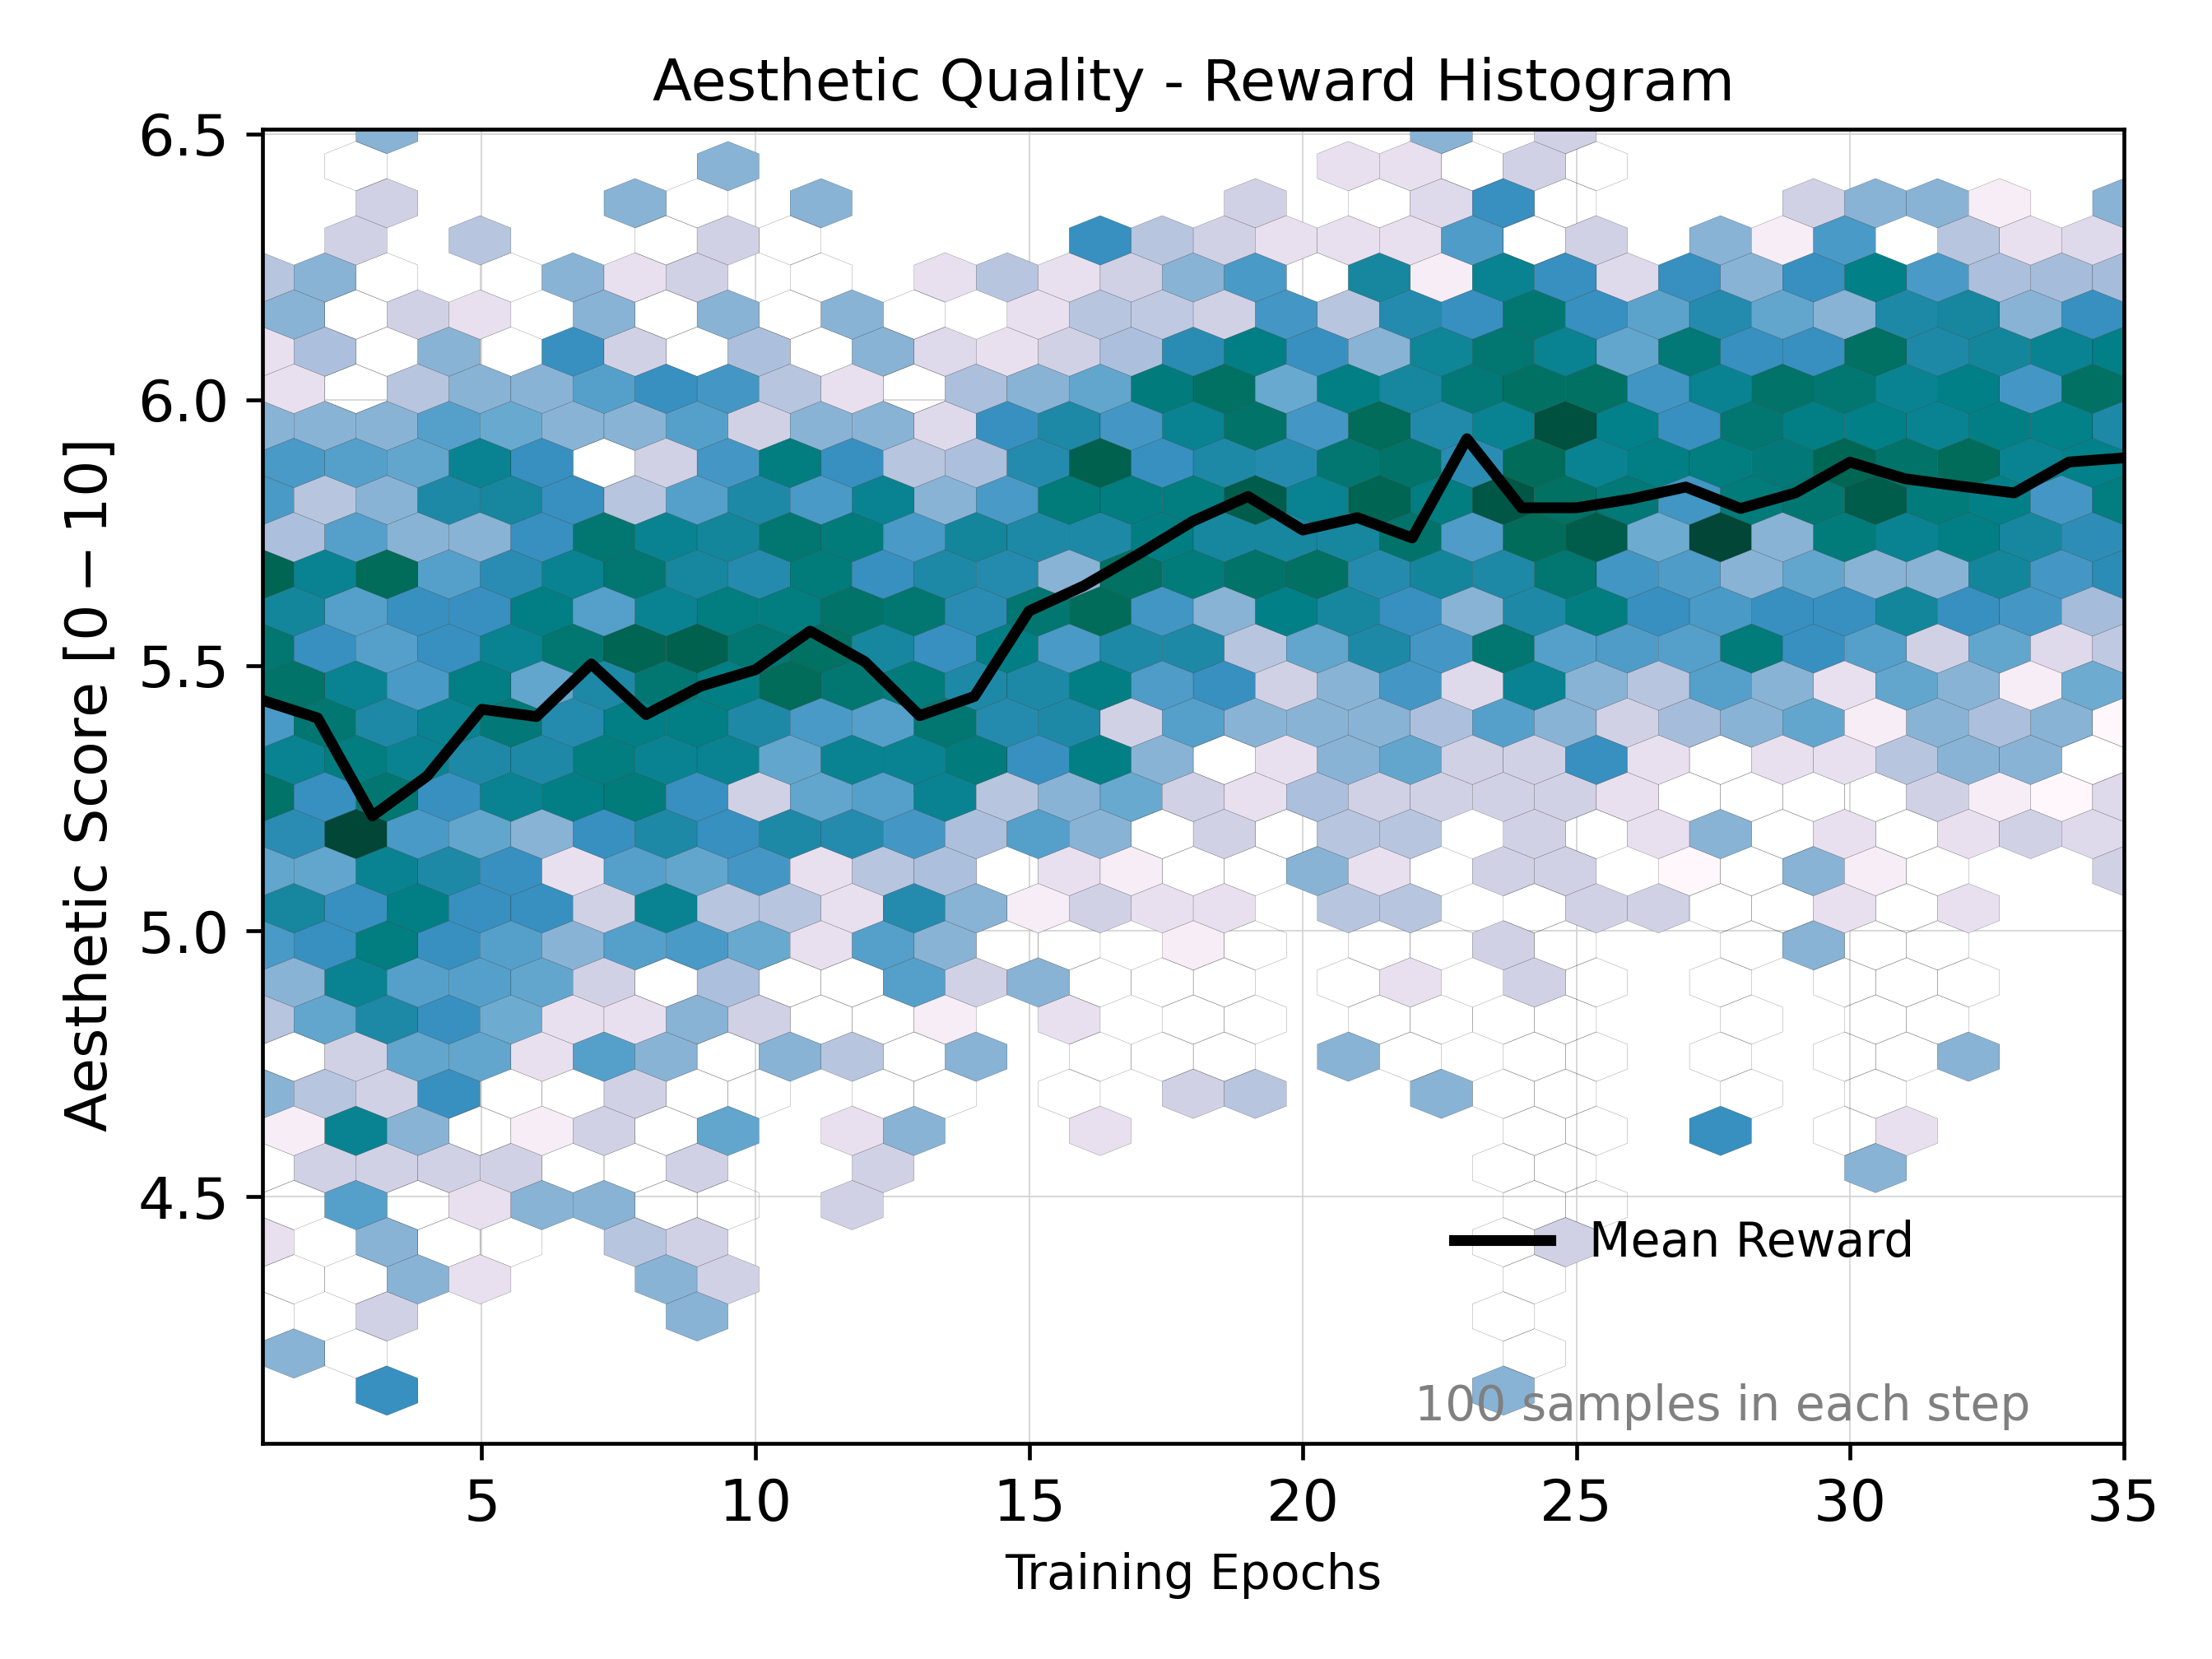
\includegraphics[width=1\textwidth]{img/results/reward_hist-laion-aesthetic.png} % first figure itself
      %\label{fig:sample_figure_1}
  \end{minipage}\hfill
  \begin{minipage}{0.5\textwidth}
      \centering
      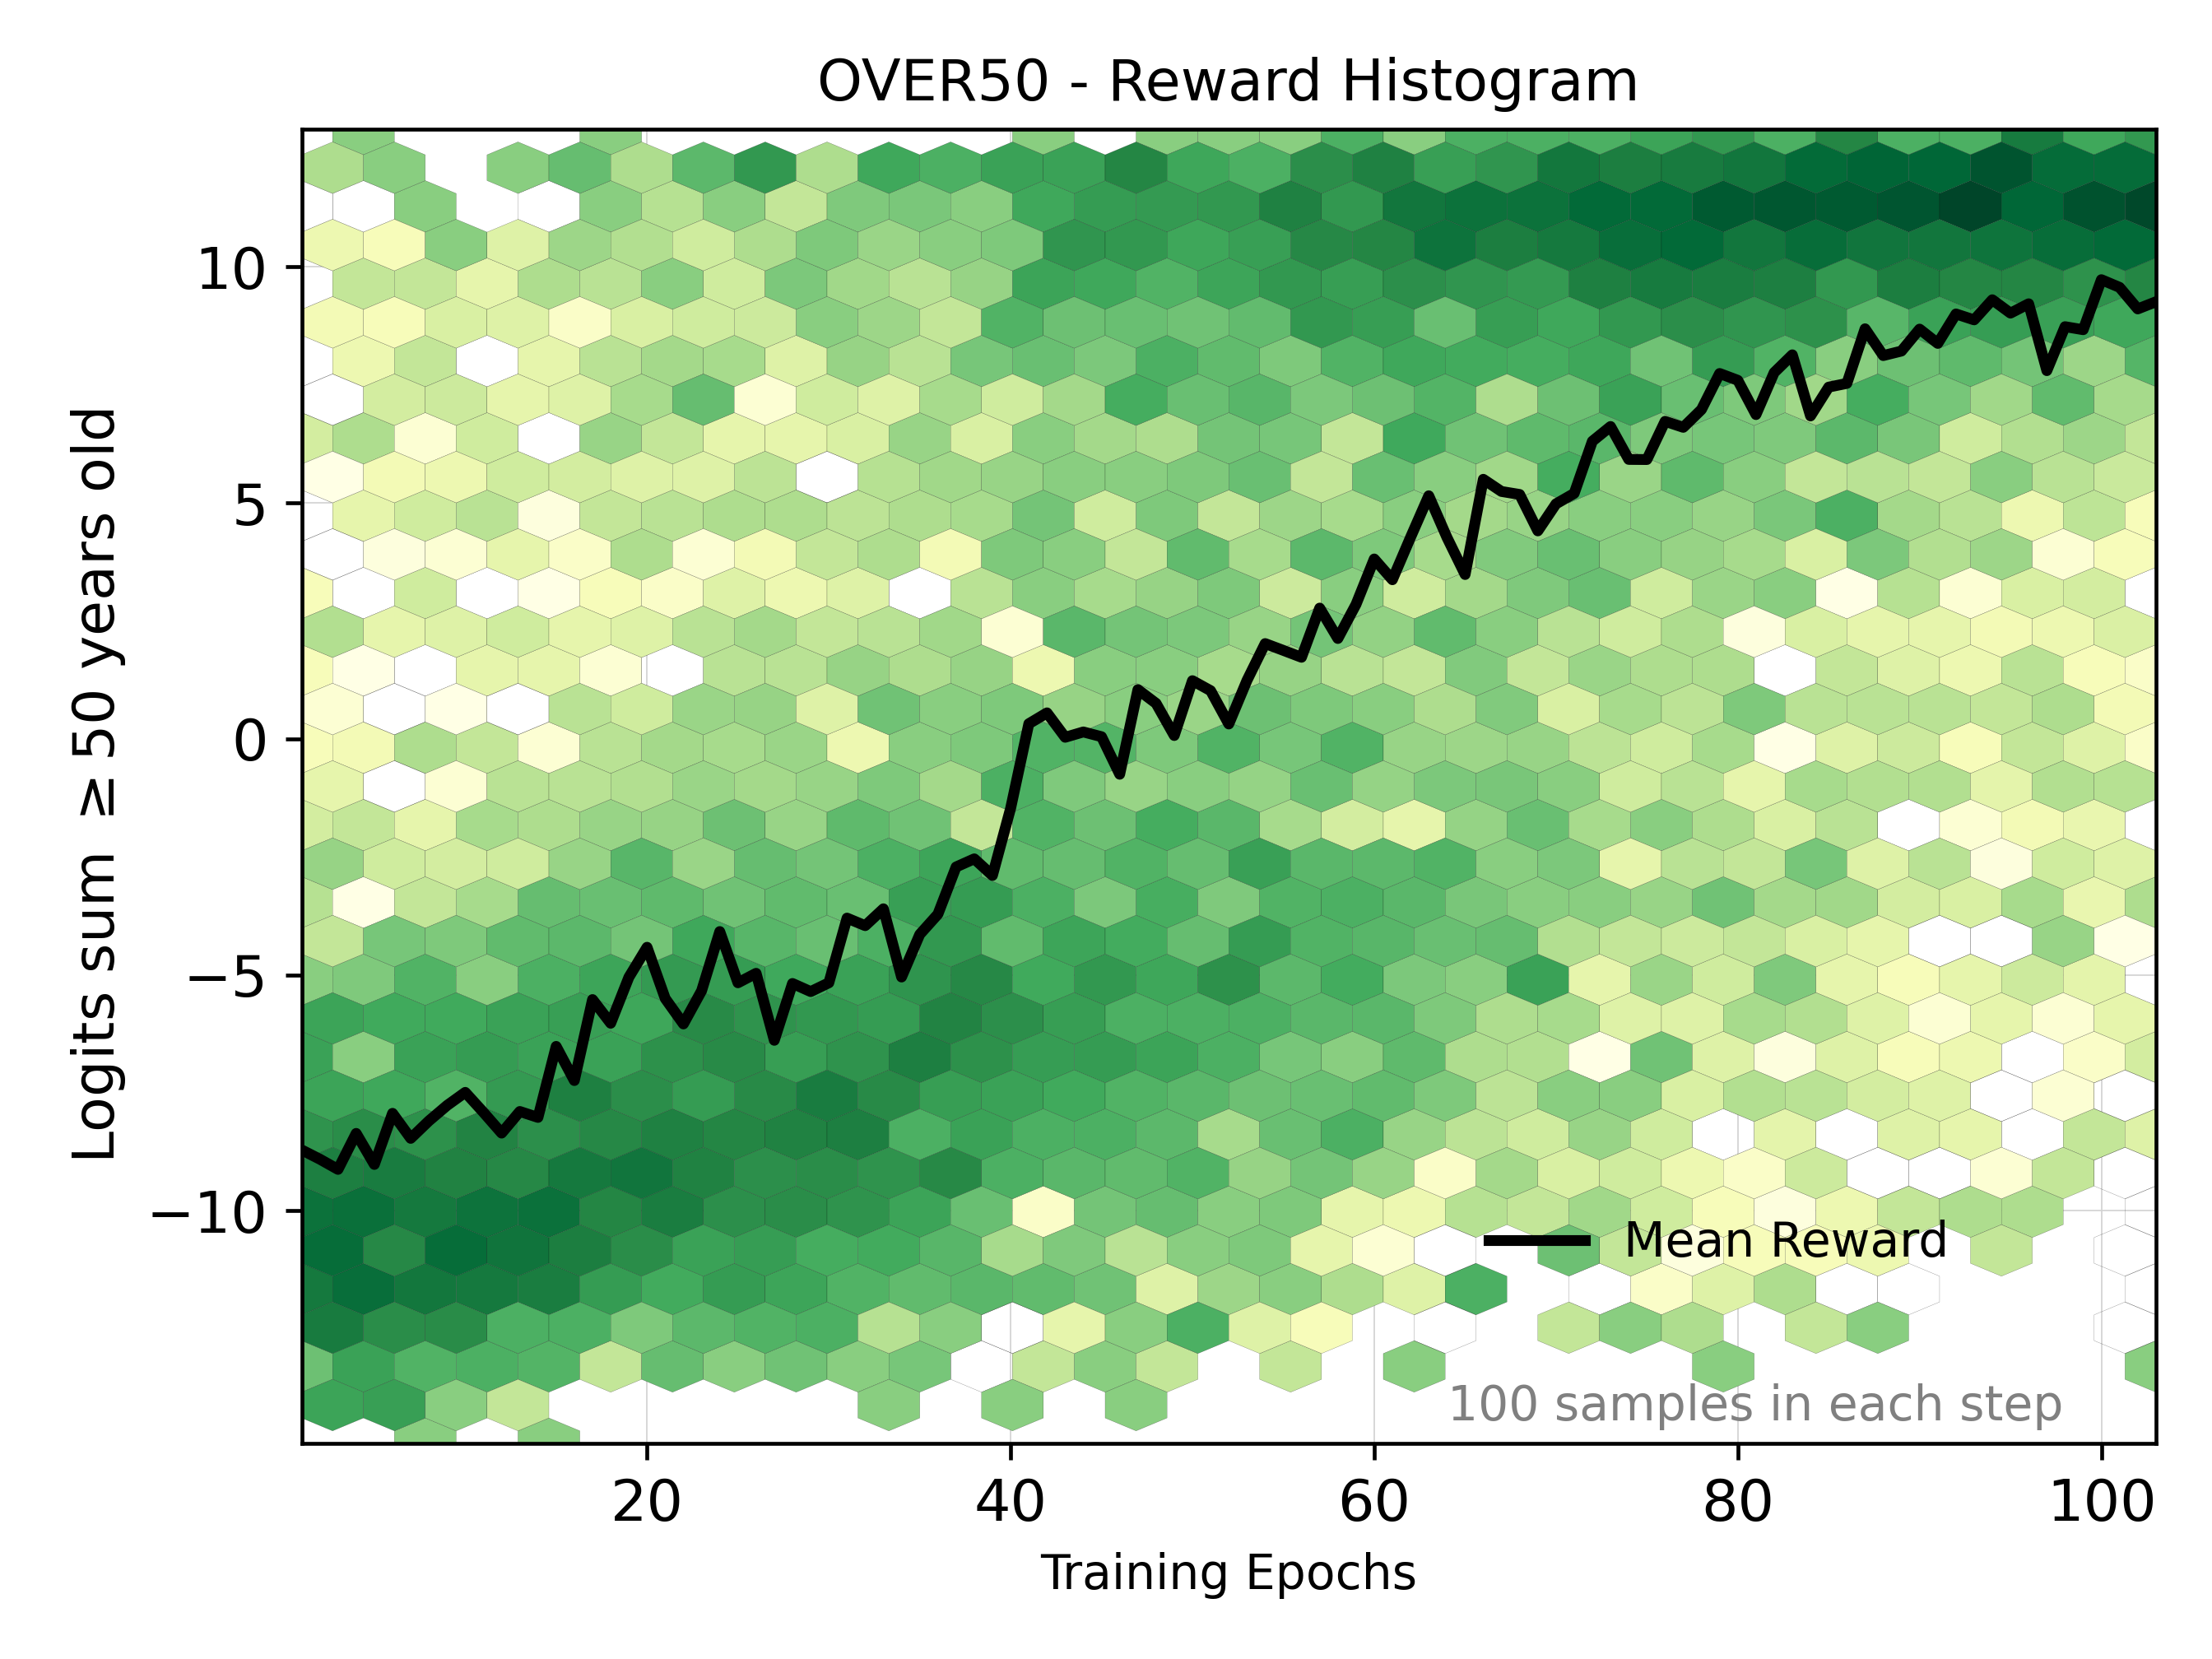
\includegraphics[width=1\textwidth]{img/results/reward_hist-over50.png} % second figure itself
      %\label{fig:sample_figure_2}
  \end{minipage}\vspace{-0.1cm} % space between row 1 and row 2 of figures
  \begin{minipage}{0.5\textwidth}
      \centering
      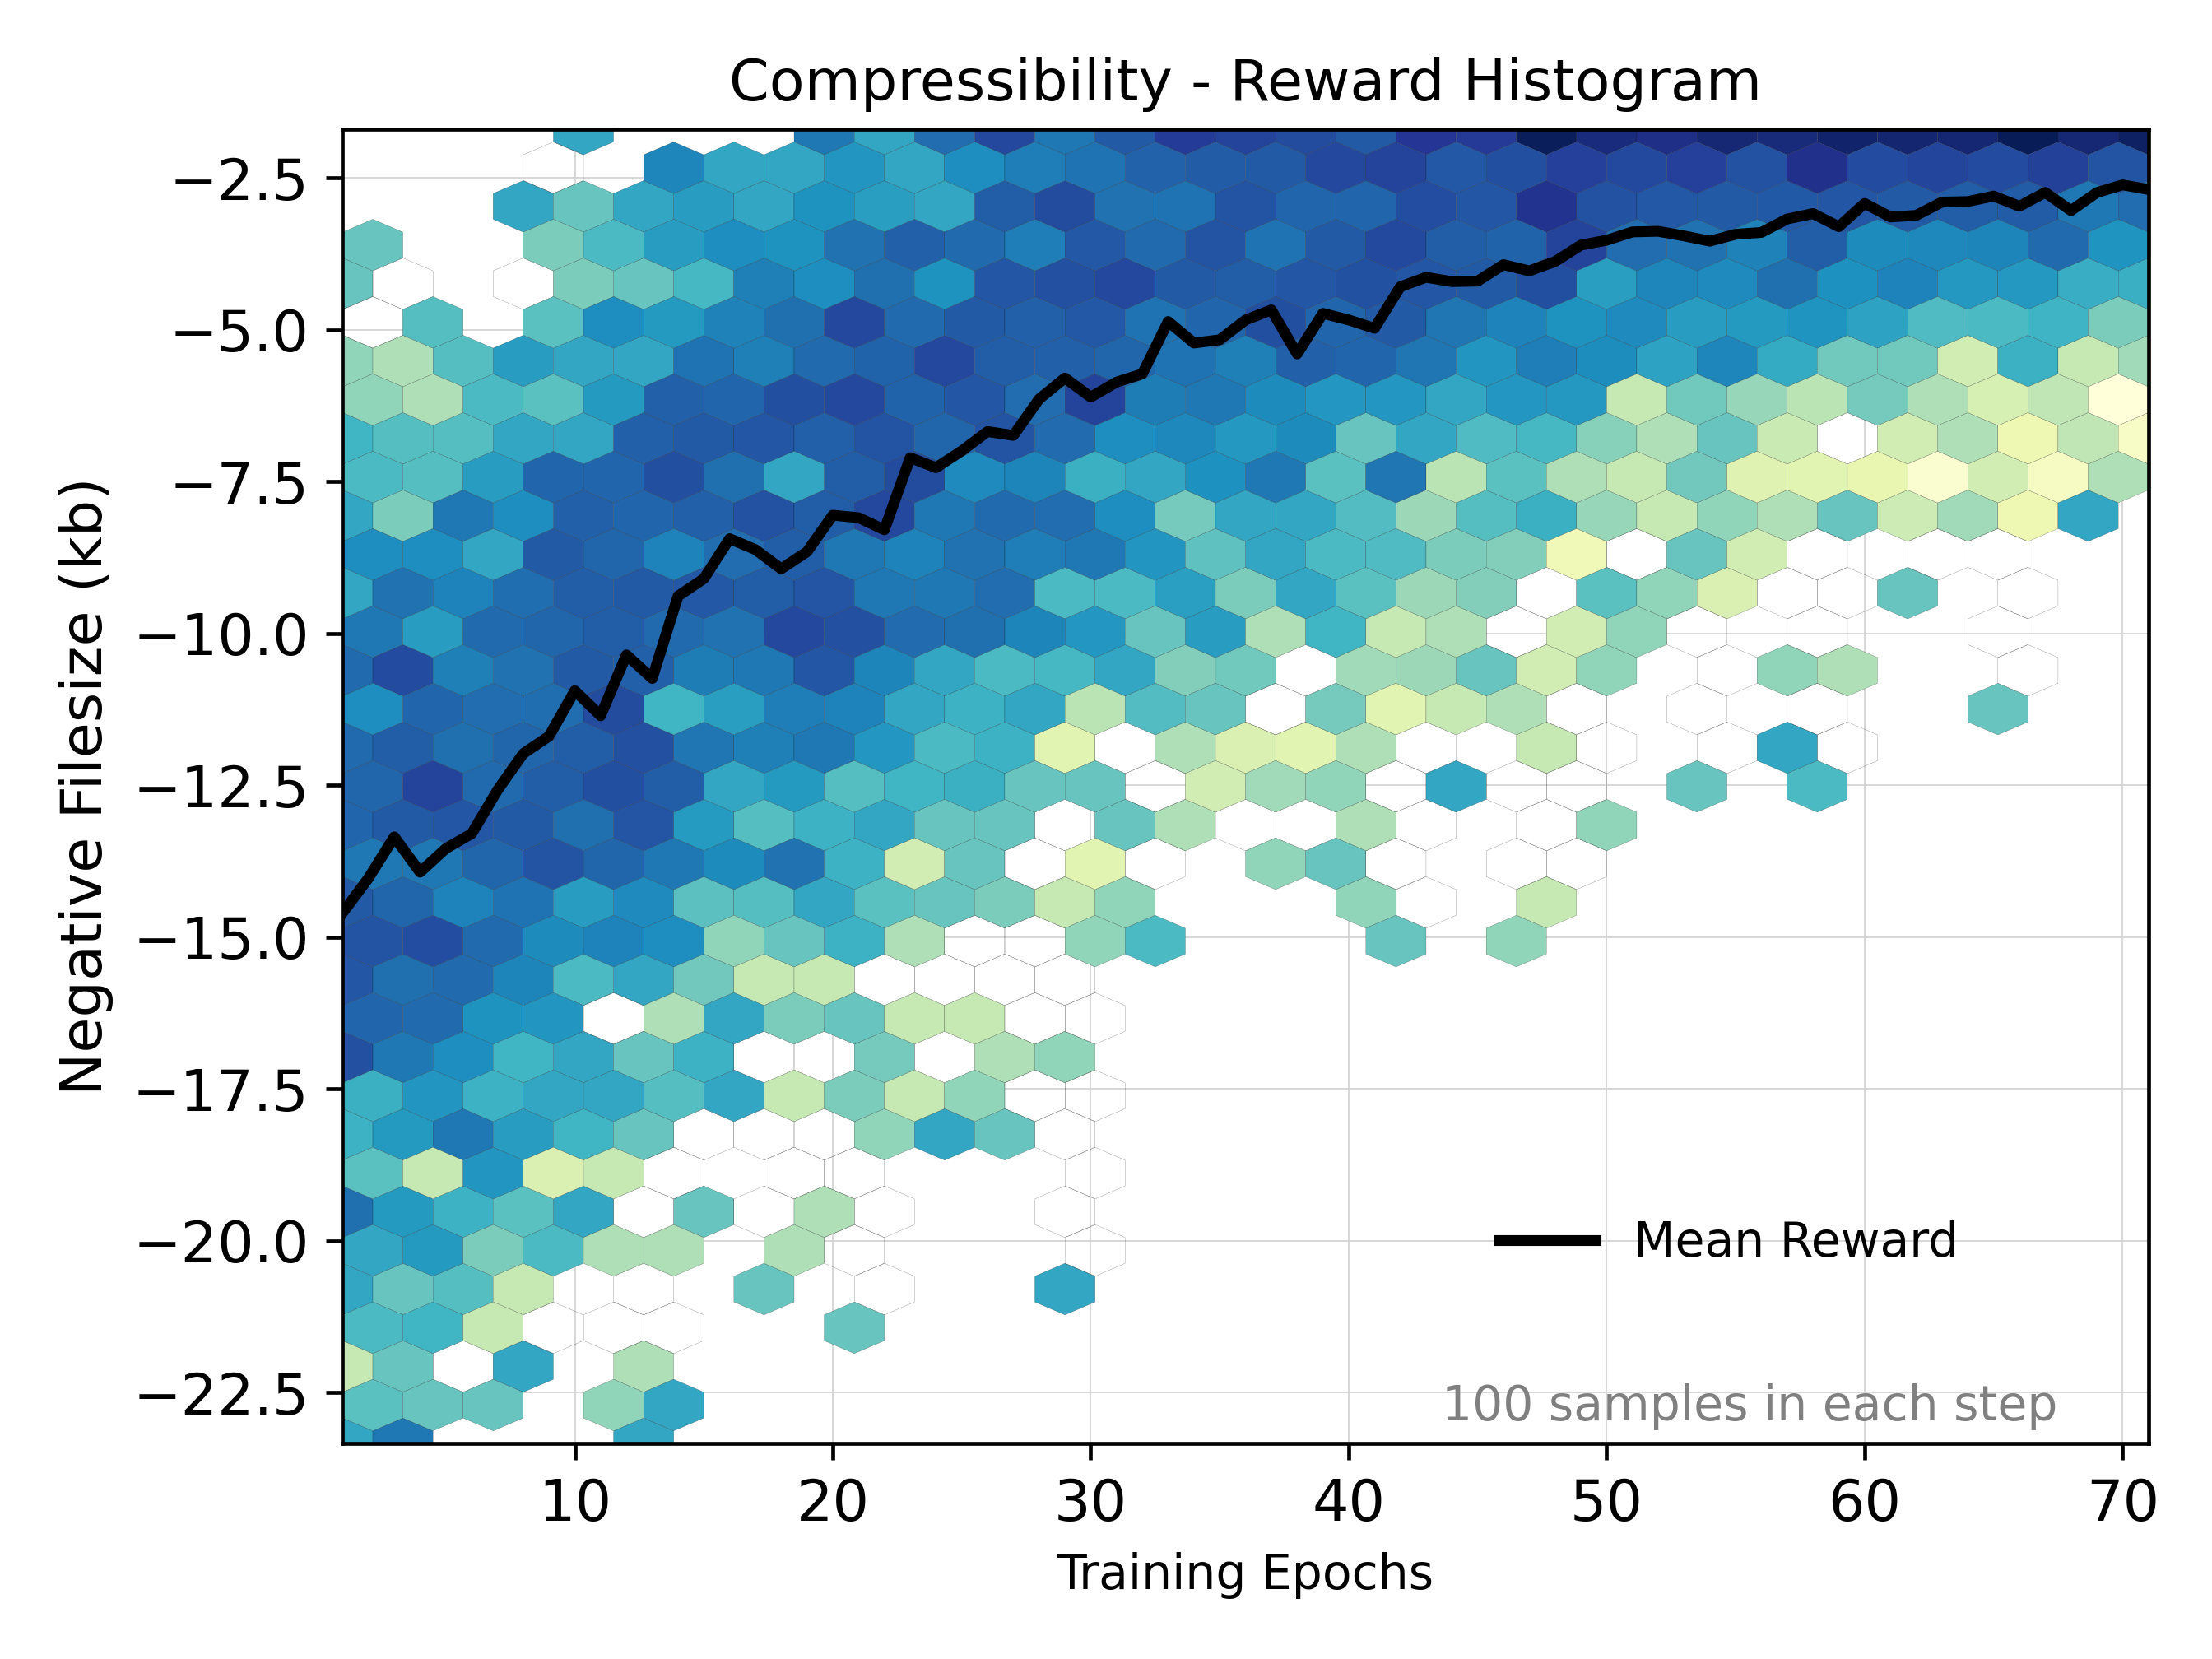
\includegraphics[width=1\textwidth]{img/results/reward_hist-jpeg-compressibility.png} % third figure itself
      %\label{fig:sample_figure_3}
  \end{minipage}\hfill
  \begin{minipage}{0.5\textwidth}
      \centering
      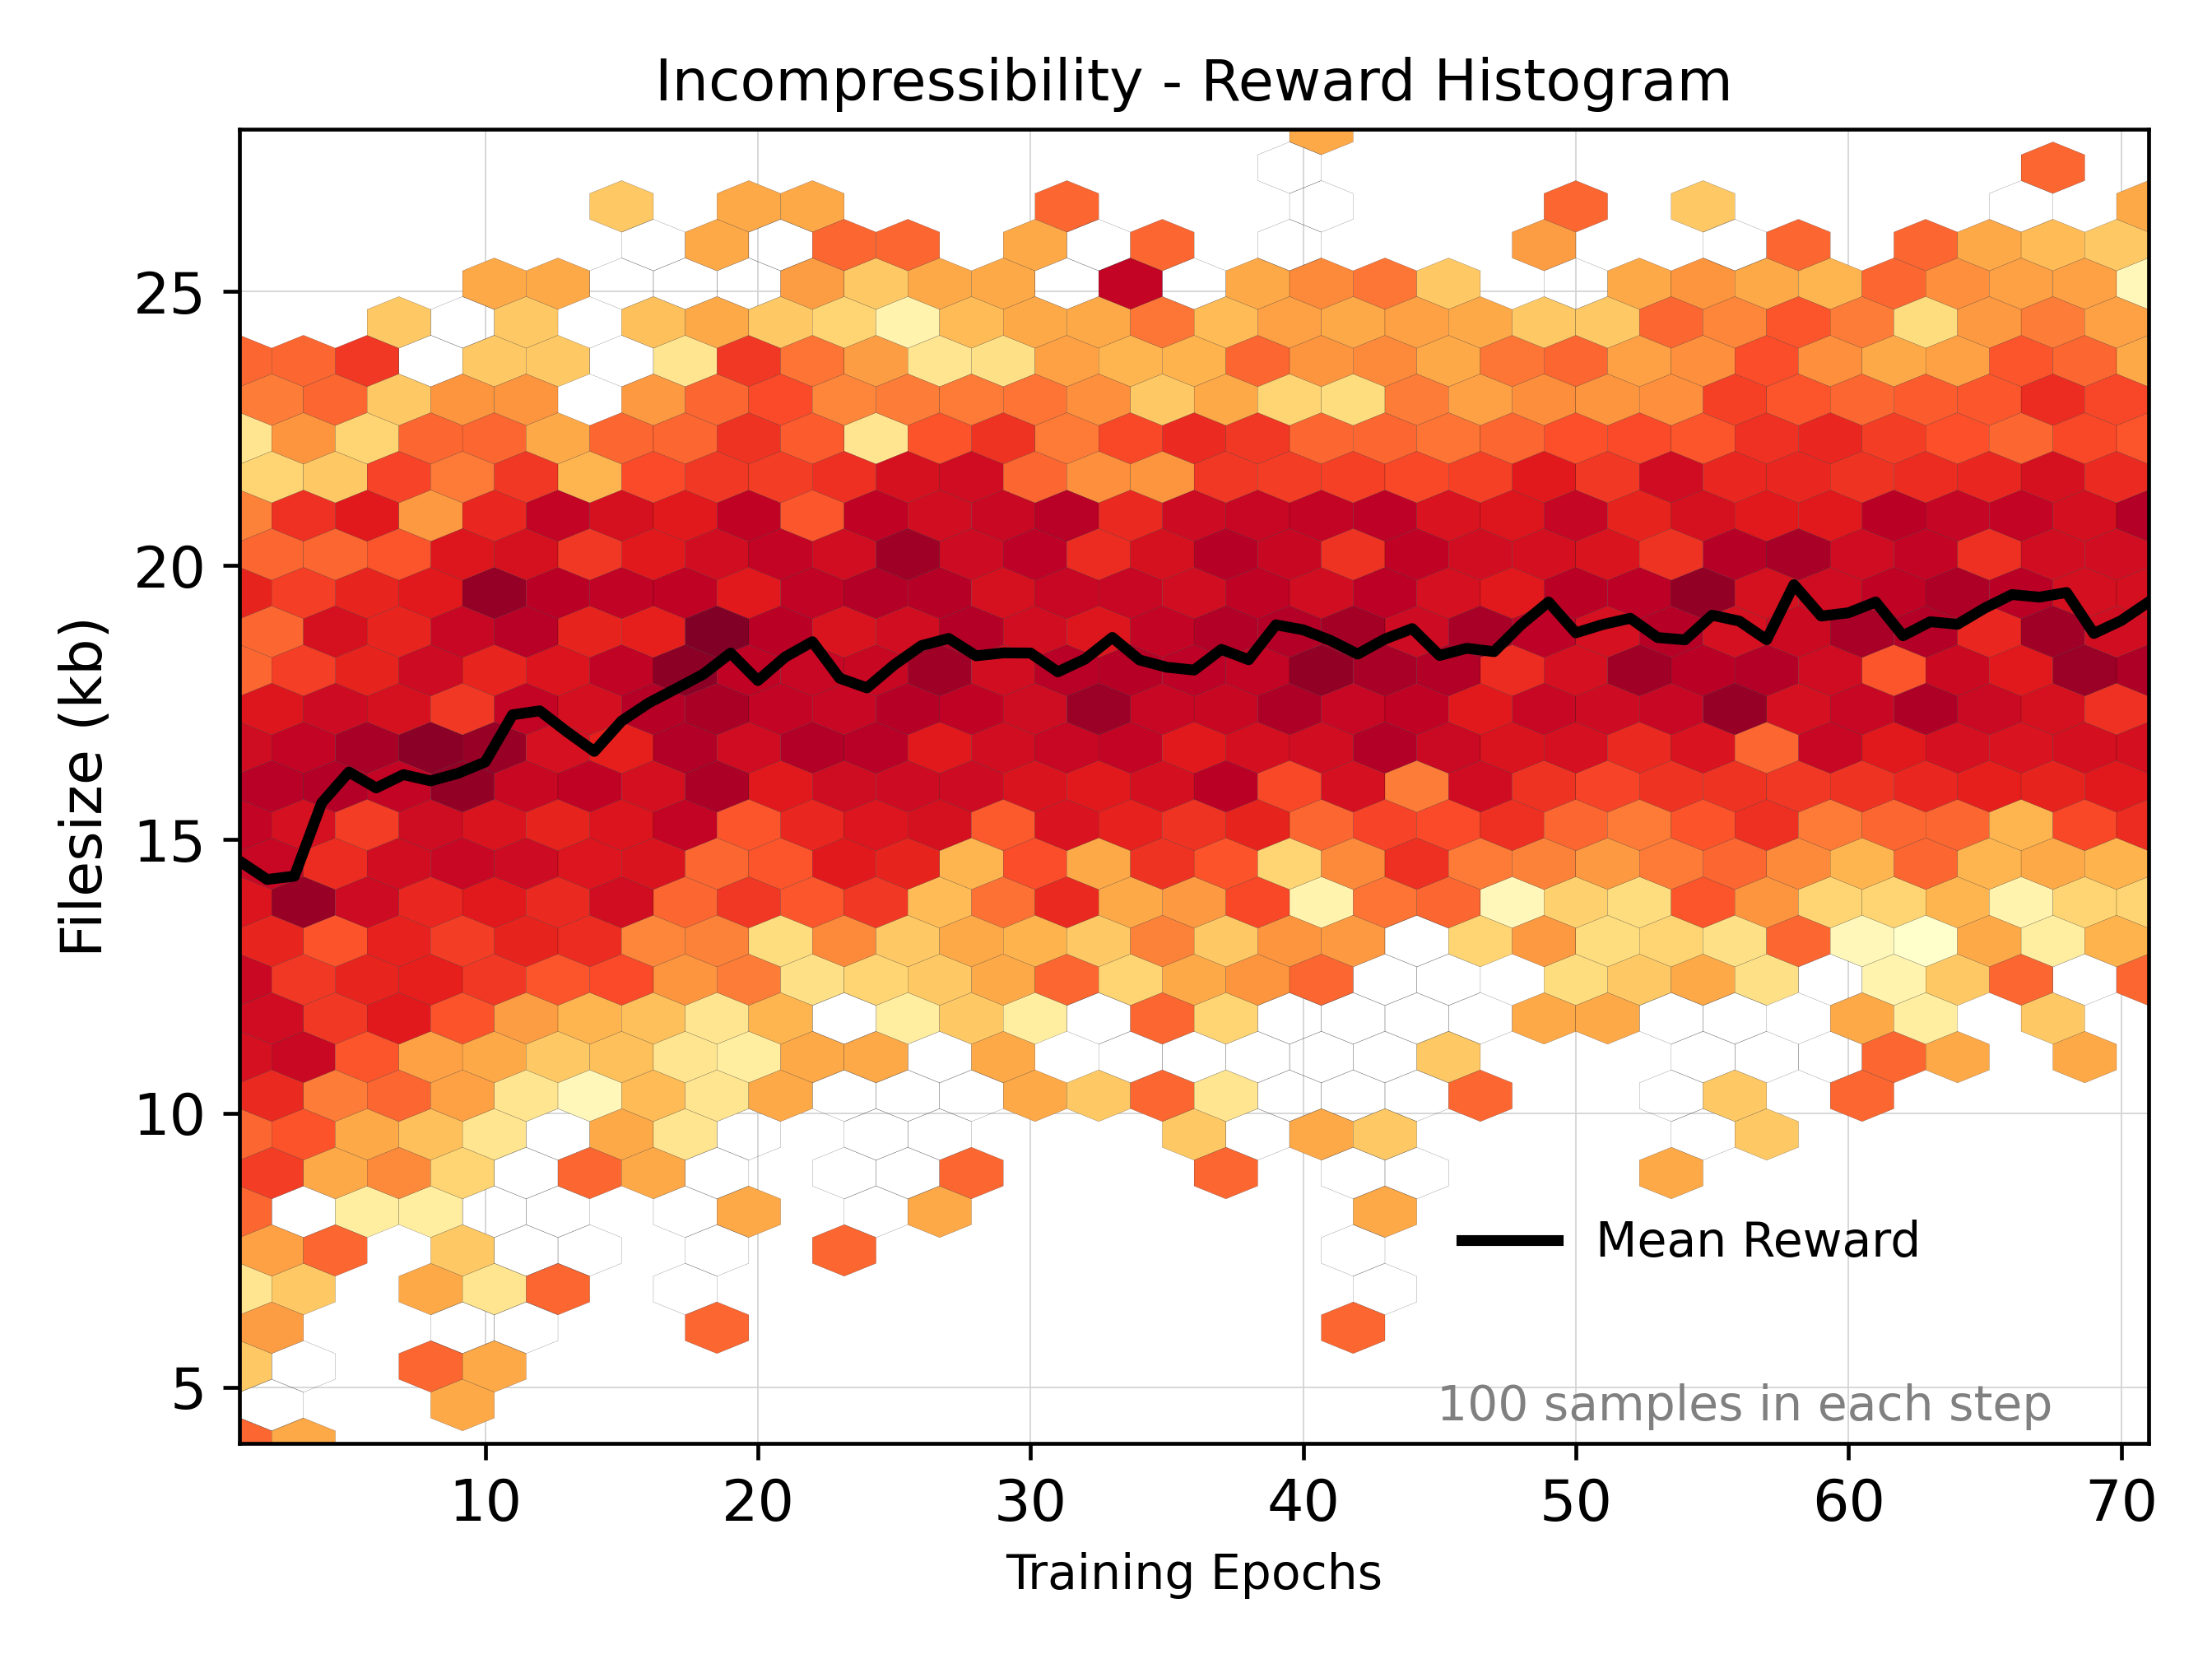
\includegraphics[width=1\textwidth]{img/results/reward_hist-jpeg-incompressibility.png} % forth figure itself
      %\label{fig:sample_figure_4}
  \end{minipage}
  \vspace{-8pt}  % reduce space between caption and figure
    \captionsetup{width=\textwidth} % set the width of the caption
    \caption{\textbf{Learning curves from DDPO.} Evolution of the mean reward (black line) and histogram during the training steps for each \textit{downstream task}. The reward estimates were computed in each step using $100$ samples from the model.}
  \label{fig:reward_hist} % Add a proper reference for the label
\end{figure}

% Transition from DDPM to DDPO samples optimized for JPEG Compressibility
\begin{figure}[ht]
  \centering
  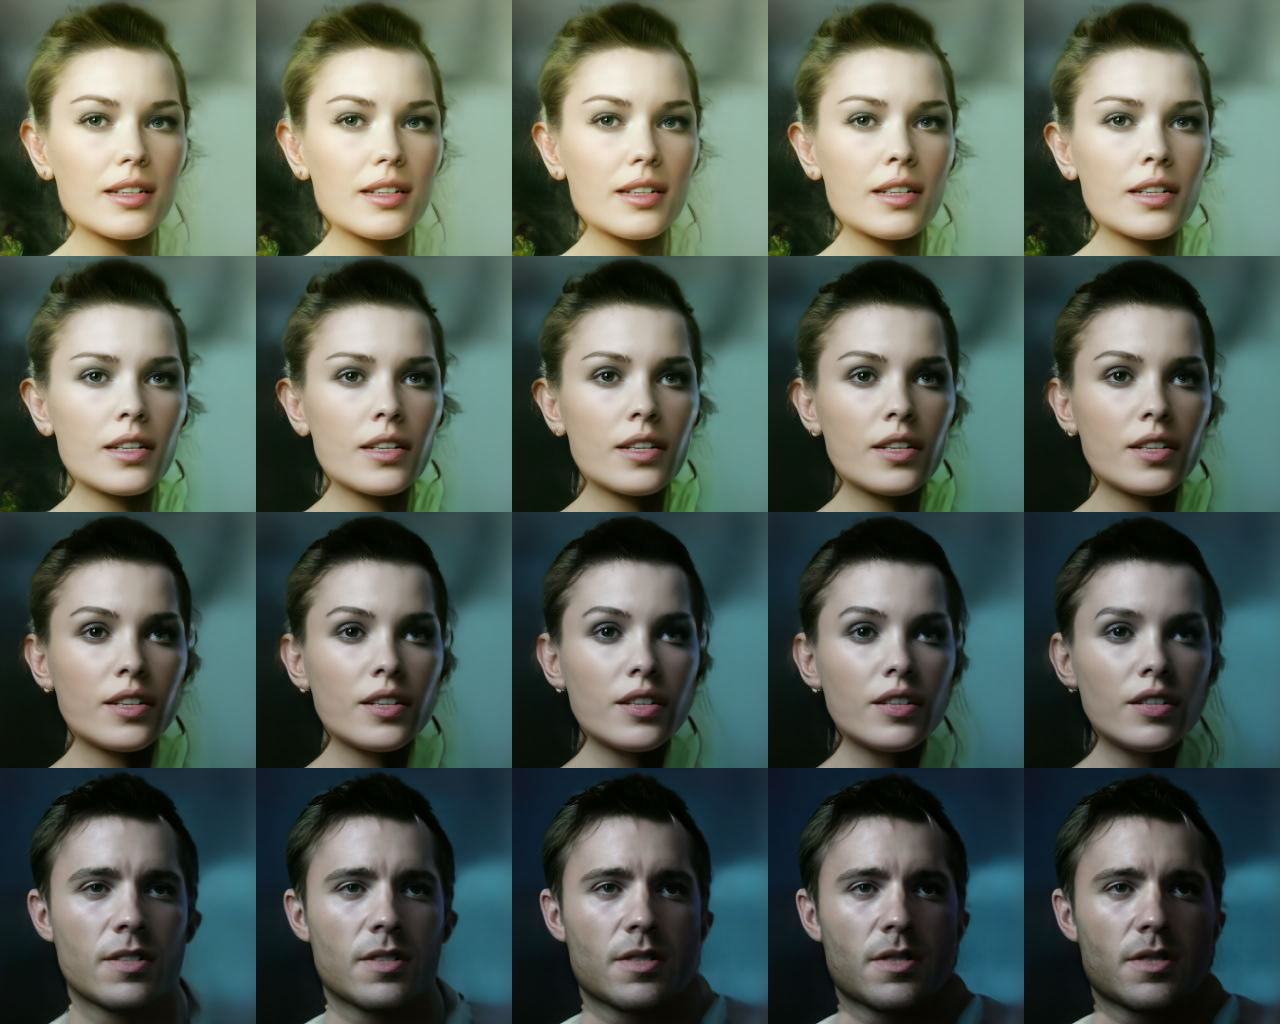
\includegraphics[scale=1.40]{img/results/compressibility_6.png}
  \vspace{-0pt}  % reduce space between caption and figure
    \captionsetup{width=\textwidth} % set the width of the caption
    \caption{\textbf{Example of JPEG compressibility transformation during model updates}, starting from \href{https://huggingface.co/google/ddpm-celebahq-256}{\texttt{\texttt{google/ddpm-celebahq-256}}}
    pretrained model and optimized to maximize the reduction in image filesize after JPEG compression using DDPO.}
    \label{fig:ddpm-to-ddpo-compressibility}
\end{figure}

\noindent \textbf{Emergent effects in face generation using JPEG Incompressibility as reward.} The effects produced by maximizing the image size using DDPO are, in some ways, the opposite of those observed when maximizing compressibility. In this case, generating images with larger file sizes is achieved through the addition of details and overall increase in brightness.
Some recurring effects during the finetuning process include adding details such
as hair voluminzation \& definition, lightening of hair tones, increasing the complexity of image backgrounds, exploiting certain artifacts in the image, removing shadows, appearance or intensifying of makeup. \\

% Effects of JPEG incompressibility
\begin{figure}[ht]
  \centering
  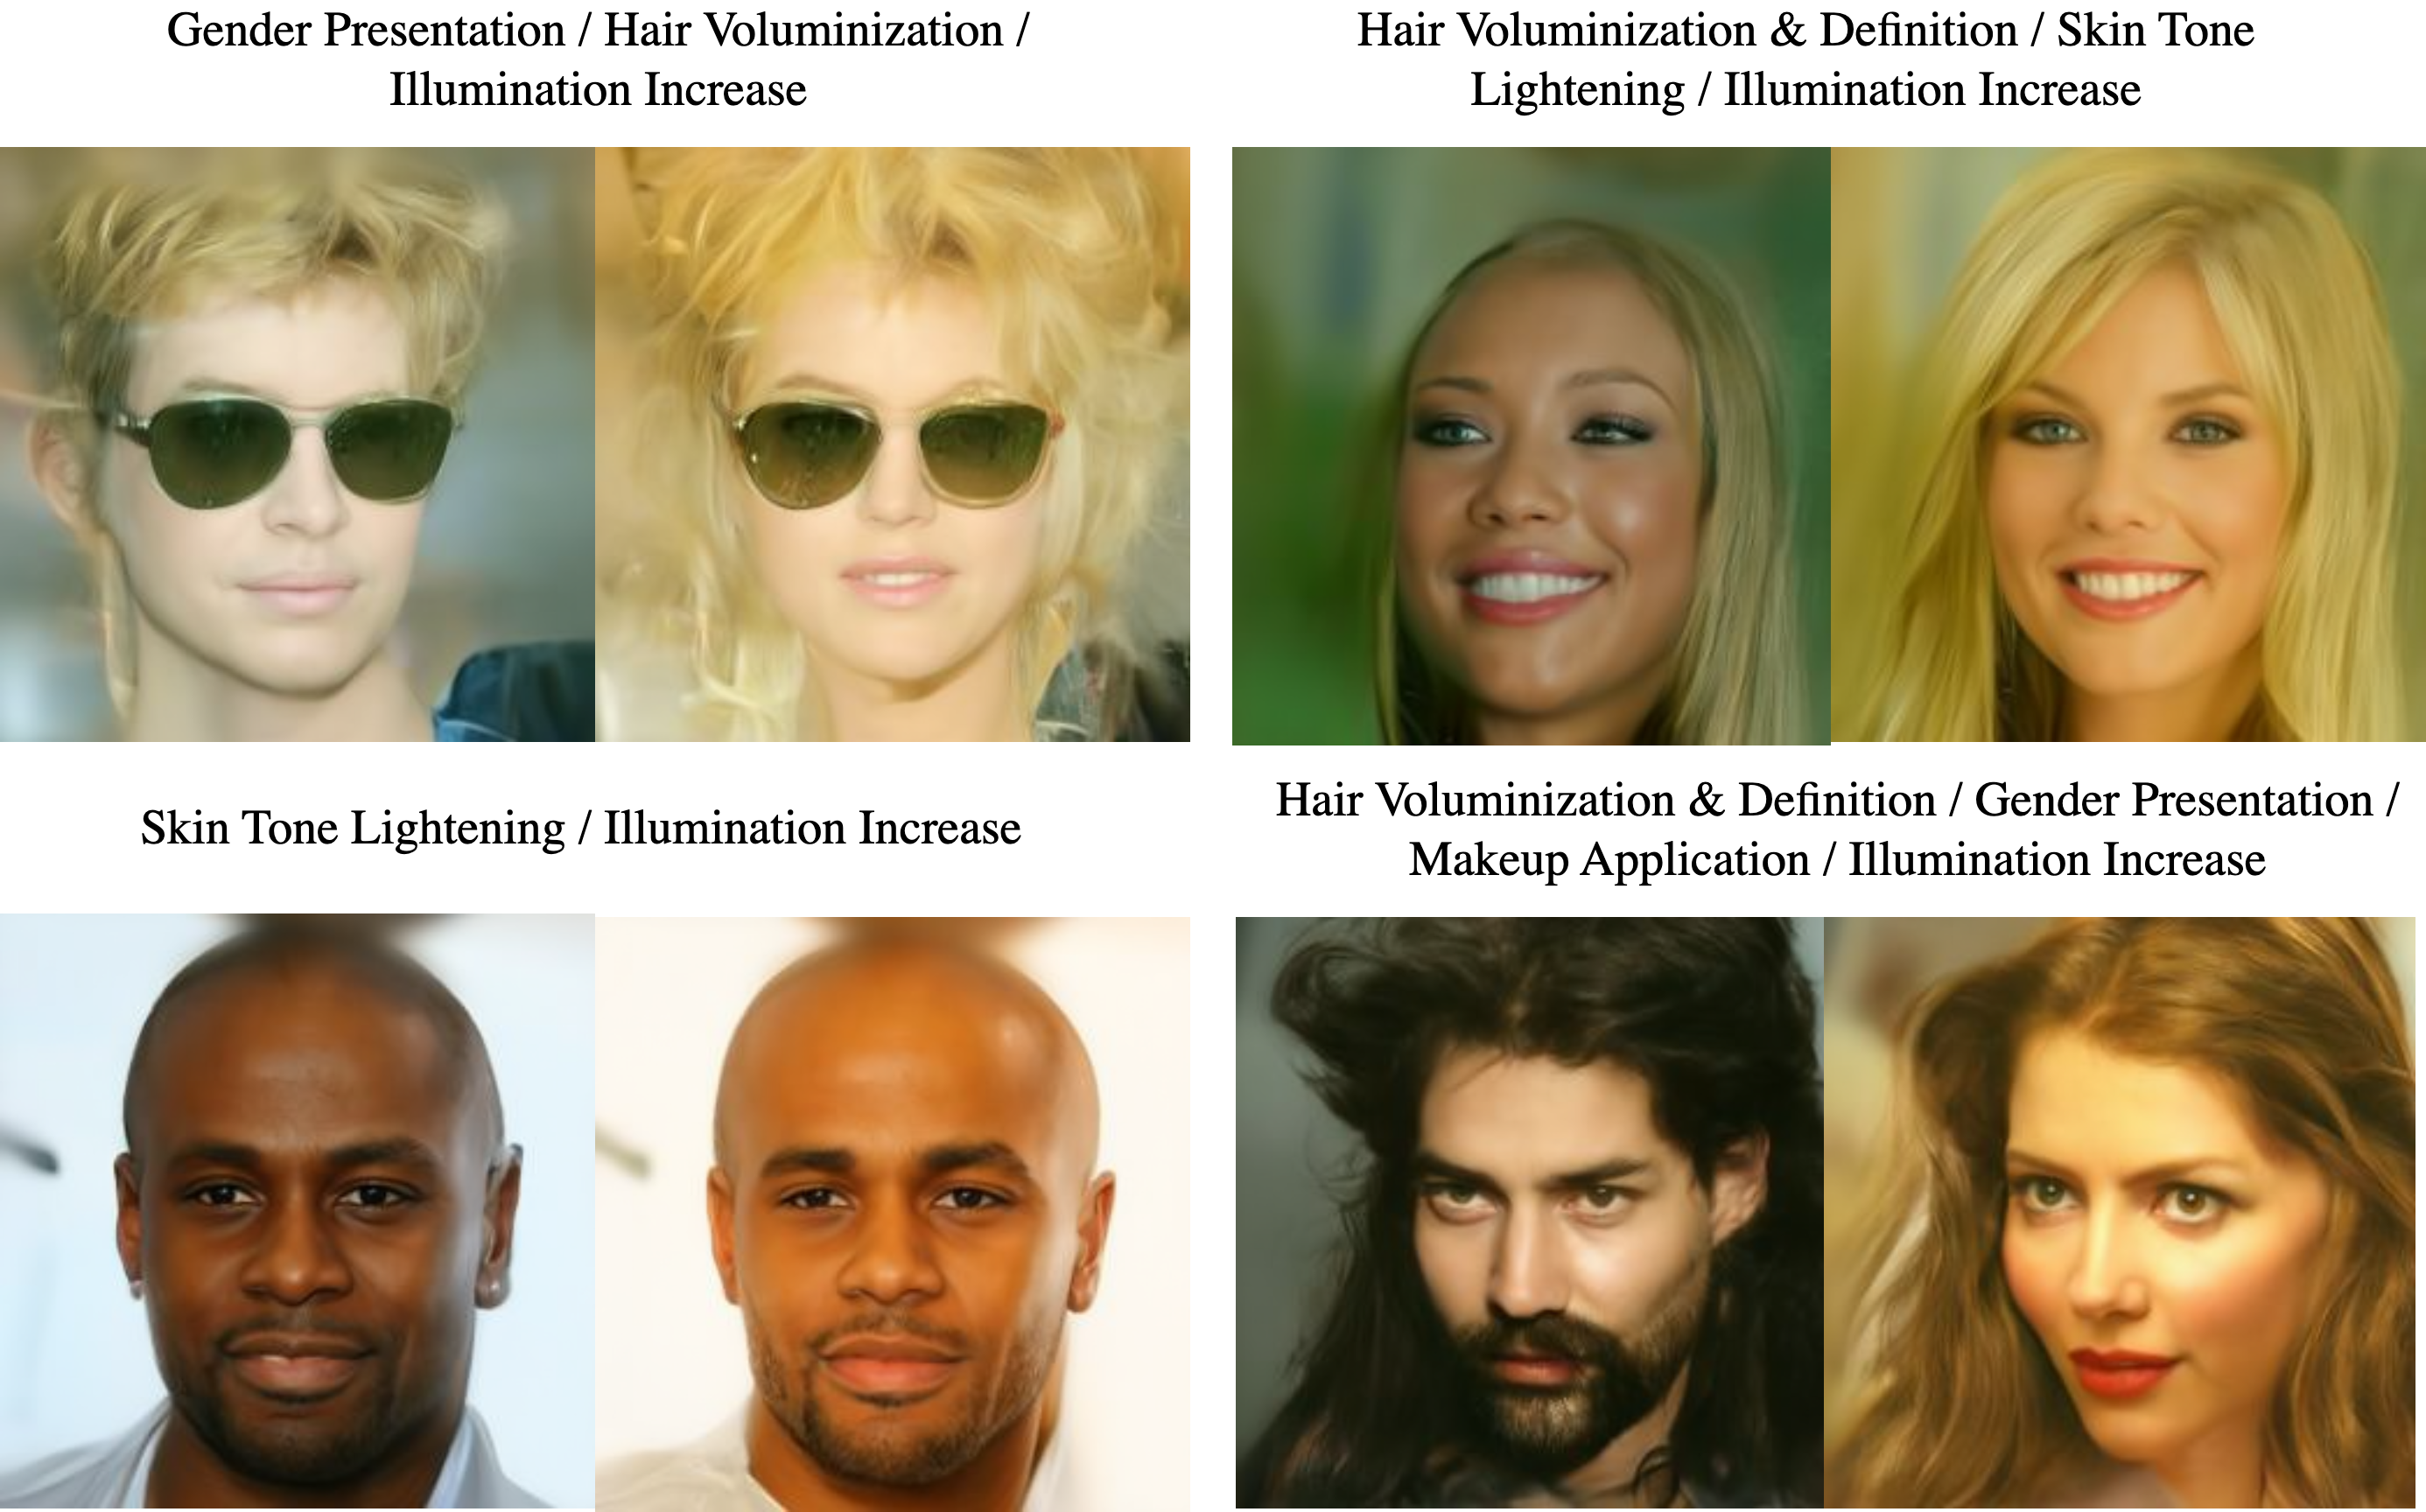
\includegraphics[scale=0.85]{img/results/incompressibility-effects.png}
  \vspace{-0pt}  % reduce space between caption and figure
    \captionsetup{width=\textwidth} % set the width of the caption
    \caption{\textbf{Emergent effects in face generation using JPEG Incompressibility as reward.} The top row shows hair volumization effects, while the right image also presents hair definition and skin tone lightening. Diagonal images illustrate gender presentation phenomena due to hair volumization and definition effects. Overall, the images show an increase in illumination and a reduction in shadows.}
    \label{fig:incompressibility-effects}
\end{figure}

\noindent The results of maximizing image size after JPEG compression are presented in Table~\ref{tab:reward-results}. It is observed that the pretrained model generates images with an average size of 17.26 kilobytes, while the finetuned DDPO model to maximize incompressibility increases the file size to an average of 21.6 kilobytes. Additionally, the reward curve of samples generated during the finetuning process is shown, indicating how the model specializes in generating larger images on average (Figure~\ref{fig:reward_hist}, red). However, even though the dispersion of rewards in the samples collected at each adjustment step decreases, incompressibility is not as effective as compressibility. Figure~\ref{fig:ddpm-to-ddpo-incompressibility}  shows the evolution of an image during the finetuning process, highlighting effects such as increased lighting, reduced shadows, greater hair definition, and the preservation of image details. Additionally, a kind of earring emerges, and artifacts in the background of the image that are difficult to compress are exploited. \\

% Transition from DDPM to DDPO samples optimized for JPEG Incompressibility
\begin{figure}[ht]
  \centering
  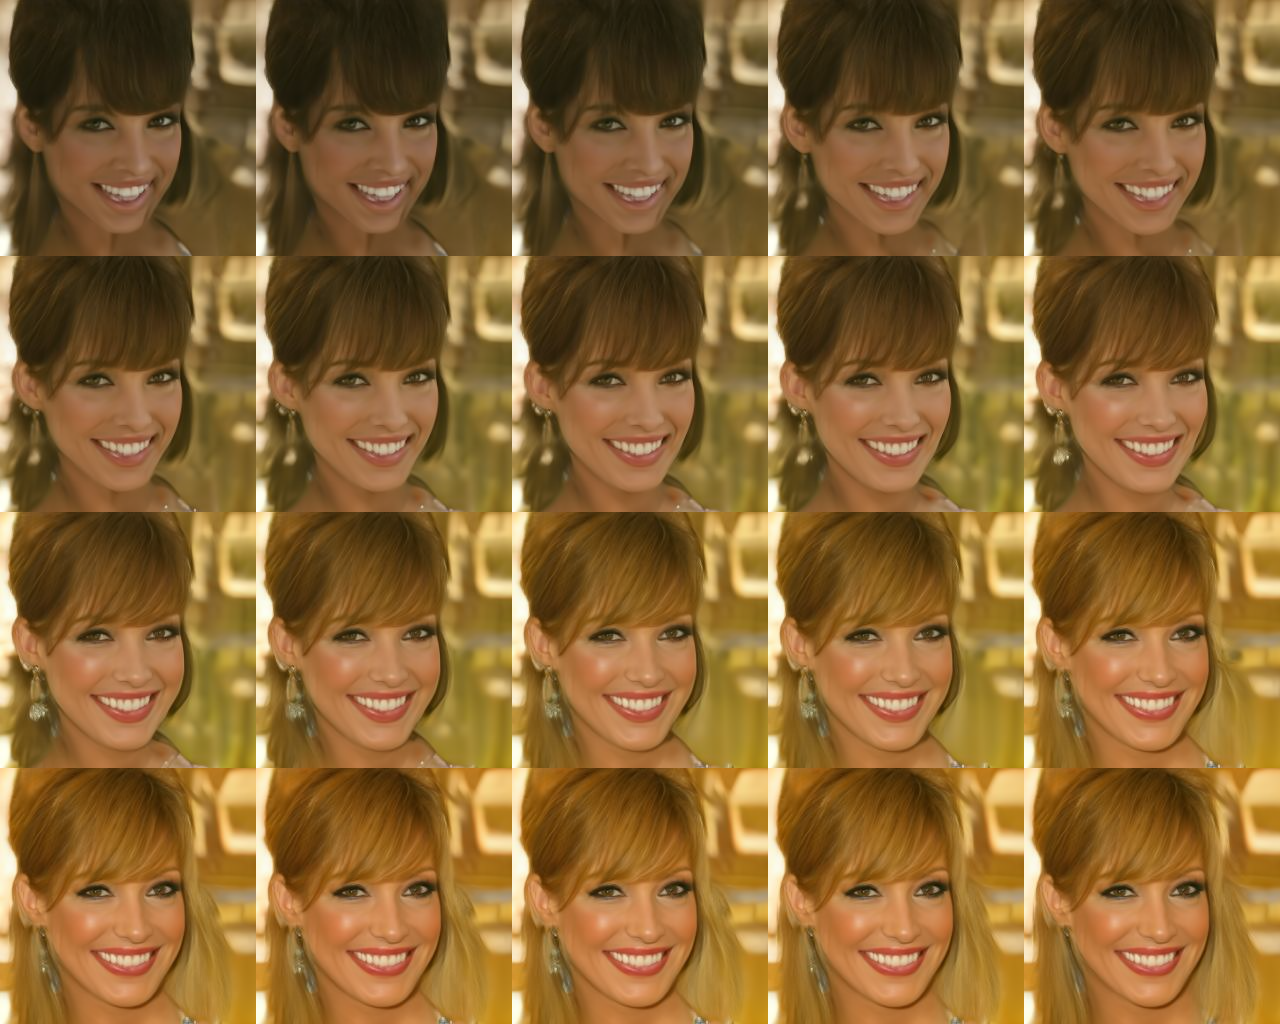
\includegraphics[scale=1.40]{img/results/incompressibility_26.png}
  \vspace{-0pt}  % reduce space between caption and figure
    \captionsetup{width=\textwidth} % set the width of the caption
    \caption{\textbf{Example of JPEG incompressibility transformation during model updates}, starting from \href{https://huggingface.co/google/ddpm-celebahq-256}{\texttt{\texttt{google/ddpm-celebahq-256}}}
    pretrained model and optimized to increase the image filesize after JPEG compression using DDPO.}
    \label{fig:ddpm-to-ddpo-incompressibility}
\end{figure}

\noindent It is interesting to compare the learning dynamics of both rewards using the JPEG compression algorithm. While they are two sides of the same coin, achieving similar magnitudes is not equally easy. The learning dynamics for the incompressibility reward are more challenging by nature than for compressibility. This is reflected in the reward curves and sample histograms during training, as mentioned before (Figure~\ref{fig:reward_hist}, bottom row). However, upon deeper reflection, this makes sense given the model's capabilities and the nature of the task. Adding more information requires greater generative capacity to incorporate visual semantics and other features into the image that are not lost during the compression process. The limitation in our generative model is that its capabilities are reduced to generating human faces and not more complex objects or scenes. On the other hand, reducing file size can always be achieved by degrading the model's generative capacity---\textit{removing information is easier than adding or creating information}. \\

% \noindent \textbf{Improving Aesthetic Quality Using RLHF.} Mejorar la 
% calidad estética de una imagen es un objetivo que puede ser alcanzado
% usando RL. Sin embargo, la calidad estética de una imagen es un atributo
% bastante subjetivo y depende de las preferencias de las personas, además de
% influencias culturales como temporales. En este tipo de situaciones en las 
% que no hay una preescripción clara para formular una función de recompensa,
% las preferencias humanas pueden ser usadas como guía para entrenar un modelo generativo. En la
% sección~\ref{sec:rlhf} se explica como las preferencias humanas pueden ser
% capturadas en un modelo de reward---\textit{en este caso un predictor de calidad estetica}---y ser utilizado para generar la señal de recompensa de las imágenes y así guiar el proceso de generación hacía la maximización del atributo en cuestión. Se realizó un ajuste del modelo prentrenado \href{https://huggingface.co/google/ddpm-celebahq-256}{\texttt{\texttt{google/ddpm-celebahq-256}}} usando LAION aesthetic predictor \cite{laion2022} para mejorar la calidad estetica de las imágenes generadas, reproduciendo el \textit{downstream task} del estudio de referencia con DDPO \cite{black2023training}. Este predictor fue entrenado sobre preferencias humanas expresadas en un score del $1$ al $10$, donde $10$ es la mejor calidad estetica\footnote{On this \href{http://captions.christoph-schuhmann.de/aesthetic_viz_laion_sac+logos+ava1-l14-linearMSE-en-2.37B.html}{site, you can find reference images} for different score ranges, providing an idea of the aesthetiic qualitiy attribute captured by this model.}. \\

\noindent \textbf{Improving Aesthetic Quality Using RLHF.} Enhancing the aesthetic quality of an image is an objective that can be achieved using Reinforcement Learning. However, aesthetic quality is highly subjective, depending on personal preferences and cultural or temporal influences. In situations where a clear reward function is not easily formulated, human preferences can guide the training of a generative model. Section~\ref{sec:rlhf} explains how human preferences can be captured in a reward model and used to generate the reward signal for images, thus guiding the generation process to maximize the desired attribute. \\

\noindent We finetuned the pretrained \href{https://huggingface.co/google/ddpm-celebahq-256}{\texttt{\texttt{google/ddpm-celebahq-256}}} using the LAION aesthetic predictor \cite{laion2022} to enhance the aesthetic quality of generated images, replicating the downstream task from the reference study with DDPO \cite{black2023training}. This predictor was trained on human preferences expressed as scores from 1 to 10, with 10 being the highest aesthetic quality\footnote{On this \href{http://captions.christoph-schuhmann.de/aesthetic_viz_laion_sac+logos+ava1-l14-linearMSE-en-2.37B.html}{site, you can find reference images} for different score ranges, providing an idea of the aesthetic qualitiy attribute captured by this model.}. \\

\noindent We started with a pretrained model that generated a set of images to evaluate their aesthetic scores and determine the model's initial capability. We then finetuned it with DDPO to maximize aesthetic quality. The results are presented in Table~\ref{tab:reward-results}, showing that the pretrained model had an aesthetic score of $5.11$, while the DDPO-finetuned model achieved a score of $5.58$ on the evaluation set. Evidence of the training dynamics is presented through the average reward trajectory of the samples used for finetuning, demonstrating the model's specialization towards its goal (Figure~\ref{fig:reward_hist}, purple). Each iteration generated a new set of images that, on average, had higher aesthetic scores and lower reward dispersion than the previous ones.

% \noindent Comenzamos con un modelo preentrenado que se genera un grupo de imágenes para evaluar su score estético y obtener la capacidad inicial del modelo. Y luego lo ajustamos con DDPO para maximizar la calidad estética. Los resultados se presentan en la Tabla~\ref{tab:reward-results}, donde se observa que el modelo preentrenado reporta un score estetico de $5.11$, mientras que el 
% modelo ajustado con DDPO alcanza un score de $5.58$ en el conjunto de 
% evaluación. Se presenta como evidencia de la dinamica de entrenamiento la 
% trayectoria de recompensa promedio de las muestras utilizadas para el ajuste, 
% donde se observa que el modelo se especializa en su objetivo (Figura~\ref{fig:reward_hist}, purple). En cada iteración que se recolecta un nuevo
% conjunto de imágenes, estas tiende en promedio a tener mayor aesthetic score que las anteriores, y una menor dispersión de las recompensas. \\

\noindent A significant difference compared to parameter tuning in previous tasks is the requirement for a more complex training dynamic to achieve higher rewards. In previous tasks, a learning rate of $9e-8$ was used, but maximizing aesthetic quality \href{https://wandb.ai/alcazar90/ddpo-aesthetic-ddpm-celebahq256/runs/omta8esy}{did not show an increase in rewards} with the same computational budget and a learning rate of $7e-8$. On the other hand, increasing the learning rate too high (e.g., \href{https://wandb.ai/alcazar90/ddpo-aesthetic-ddpm-celebahq256/runs/3lb094dk}{$1e-5$}) resulted in degraded generated images. Therefore, we implemented a linear warm-up for the learning rate, followed by a half-cosine scheduler to control and adjust the learning rate during training. This started with a learning rate of 9e-8, linearly increasing to a peak of $3.74e-5$ within the first $25\%$ of the training steps. During the remaining $75\%$ of the training, the half-cycle cosine scheduler reduced the learning rate to $9e-9$ (see Figure~\ref{fig:laion-train-dynamic}). This training dynamic allowed the use of a higher learning rate without destroying the model's generative capabilities. Consequently, the modifications resulted in more substantial semantic variations in the images to maximize the aesthetic score without compromising generative capacity, as seen in the transition from a pretrained model sample to the final checkpoint in Figure~\ref{fig:ddpm-to-ddpo-aesthetic}. This was achieved in fewer epochs than those used in previous tasks (about half). \\

% LAION learning dynamic
\begin{figure}[ht]
  \centering
  \begin{minipage}{0.5\textwidth}
      \centering
      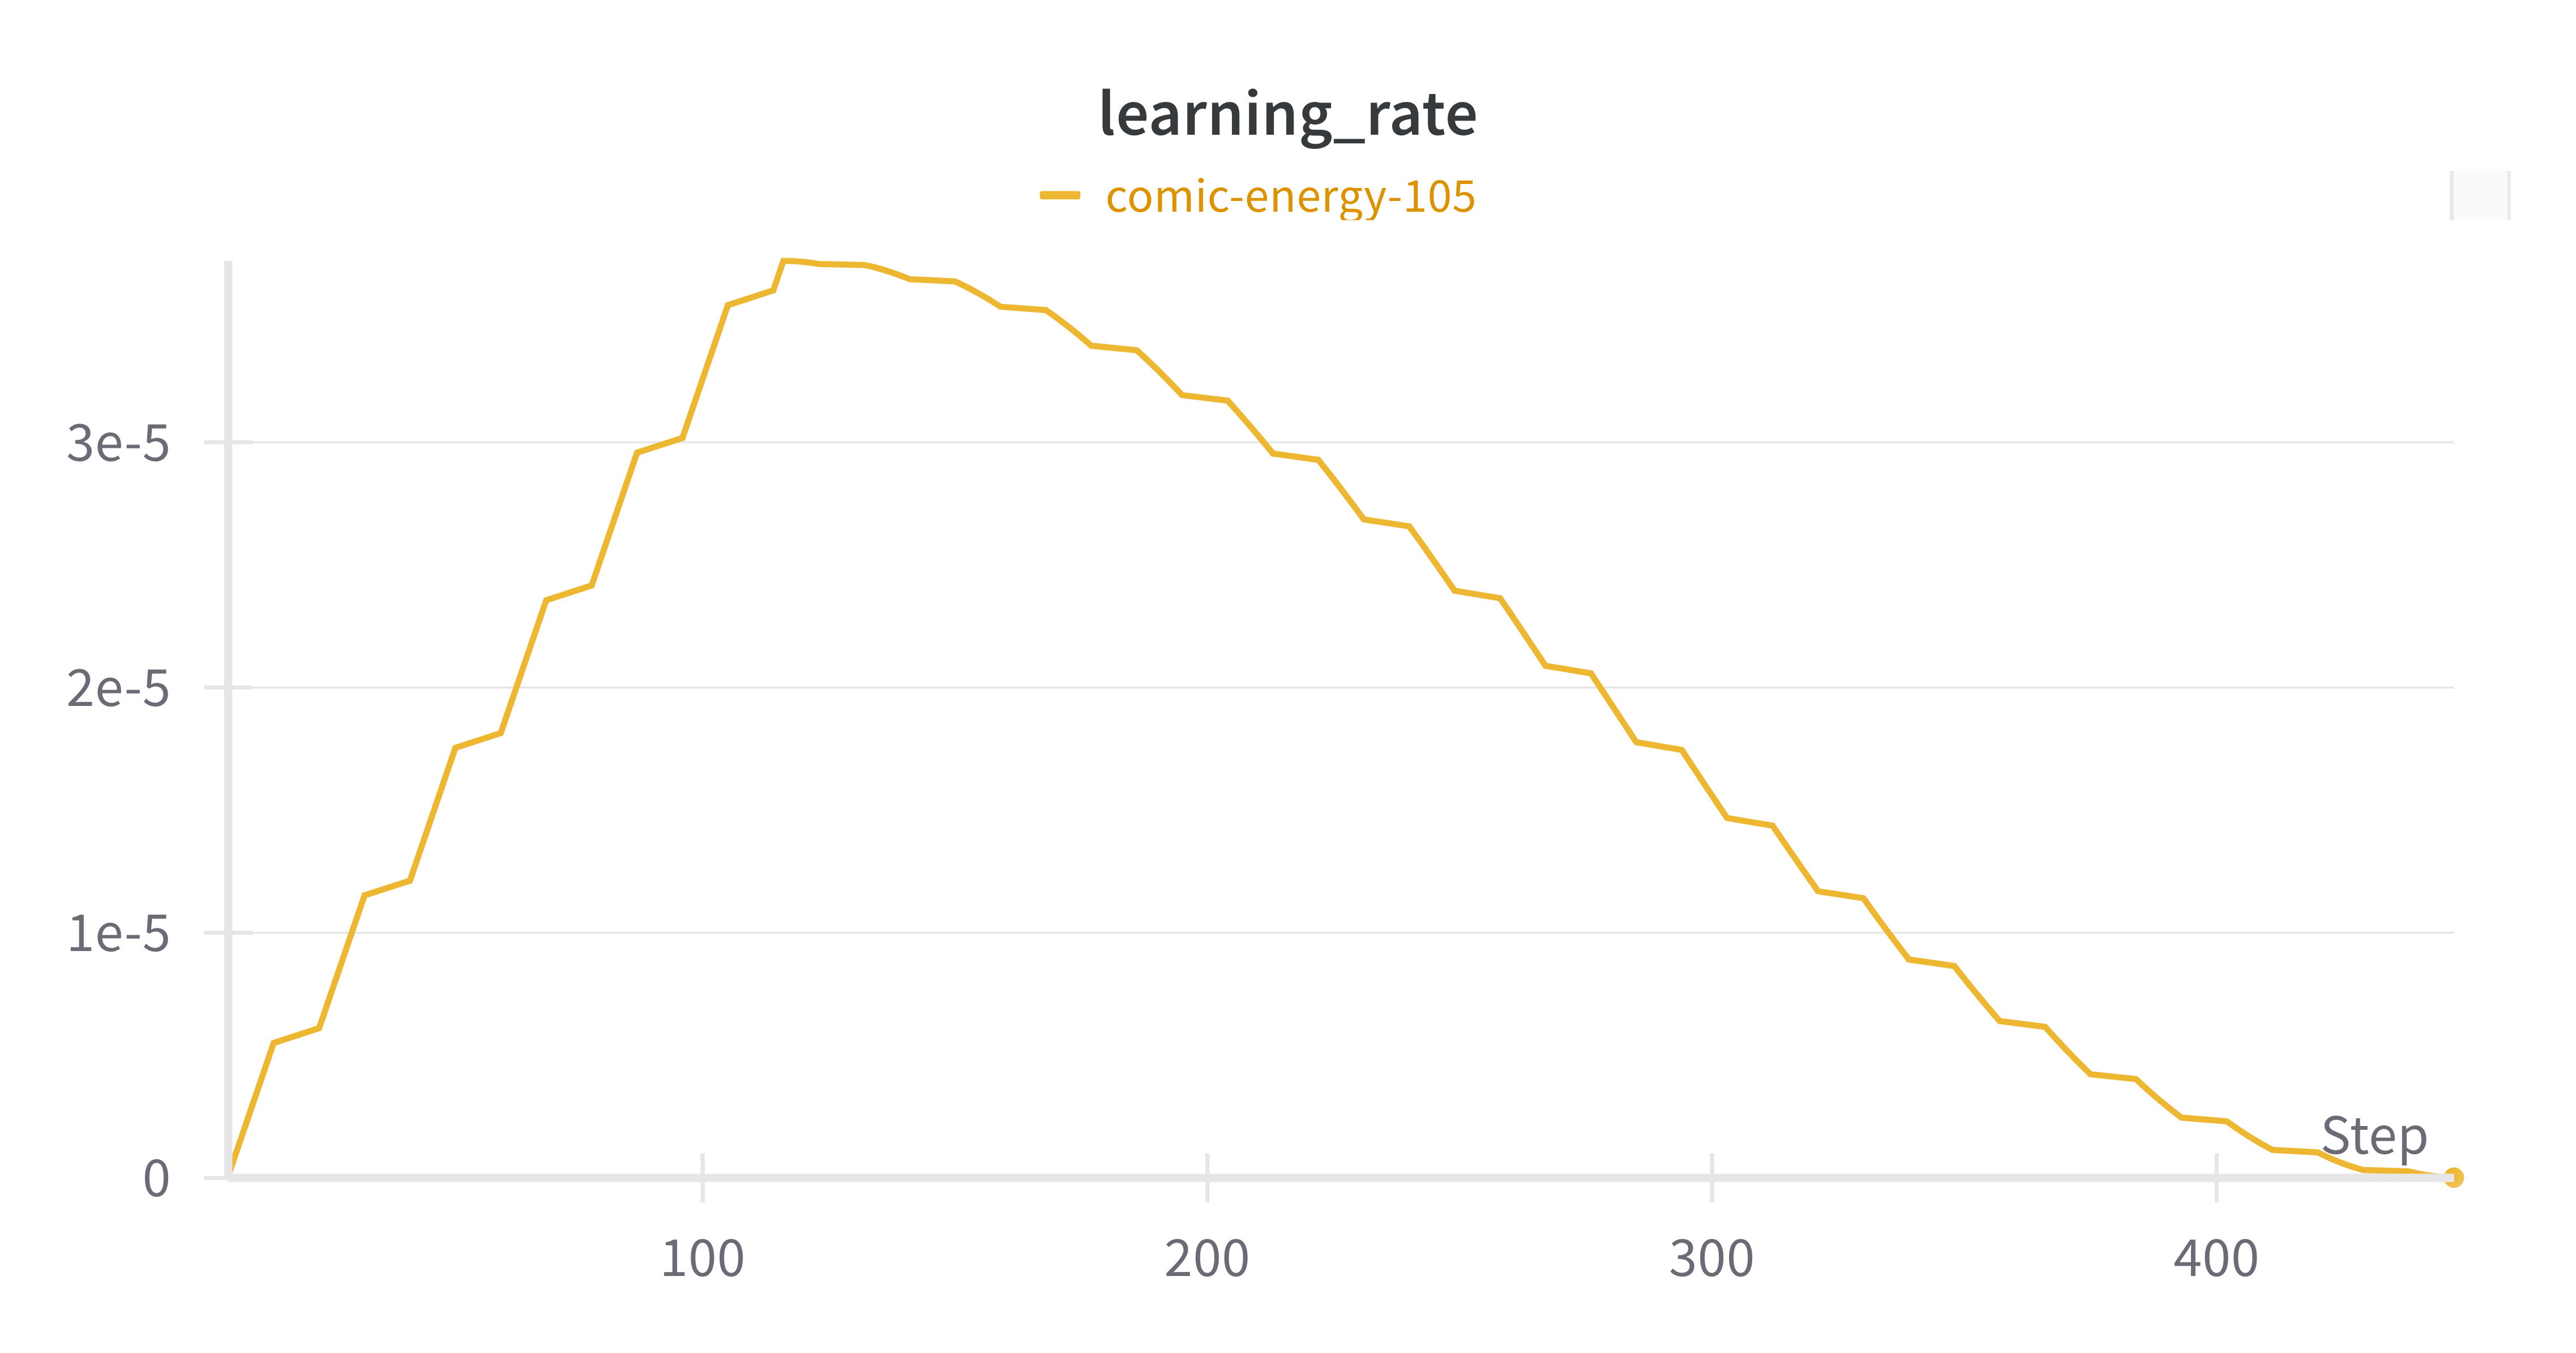
\includegraphics[width=1\textwidth]{img/results/laion-lr.png} 
  \end{minipage}\hfill
  \begin{minipage}{0.5\textwidth}
      \centering
      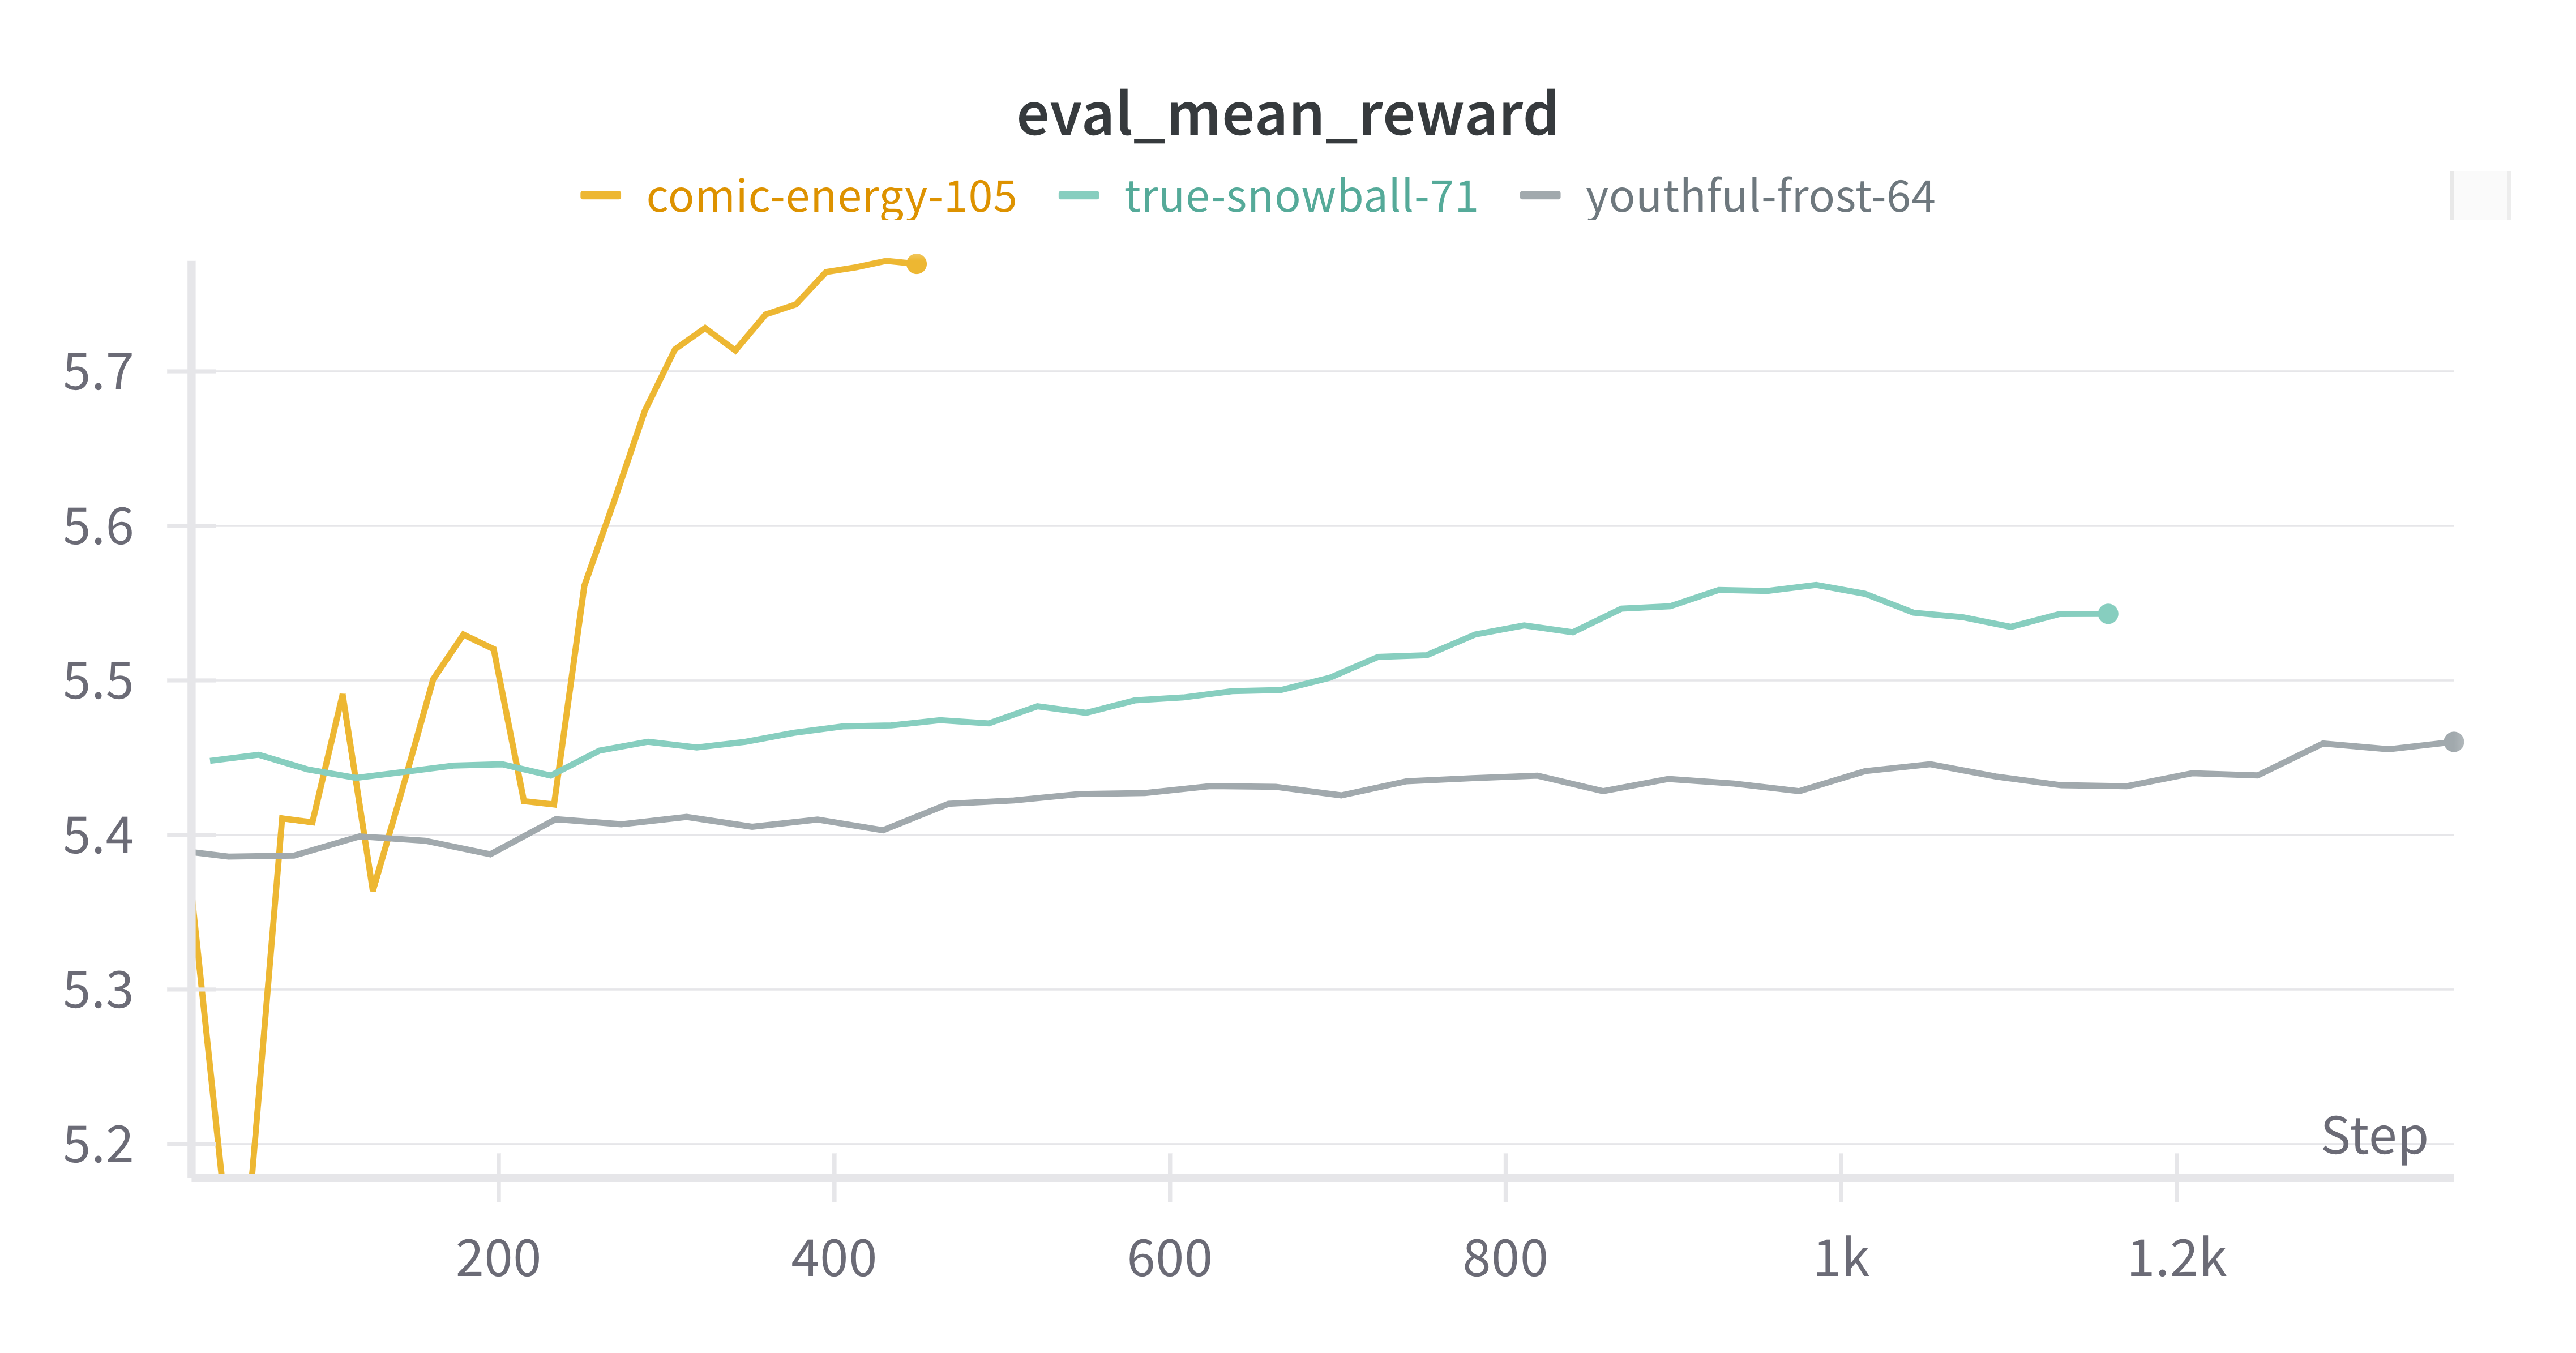
\includegraphics[width=1\textwidth]{img/results/laion-eval-mean-reward.png} 
  \end{minipage}
  % \hfill 
  % \begin{minipage}{0.2\textwidth}
  %     \centering
  %     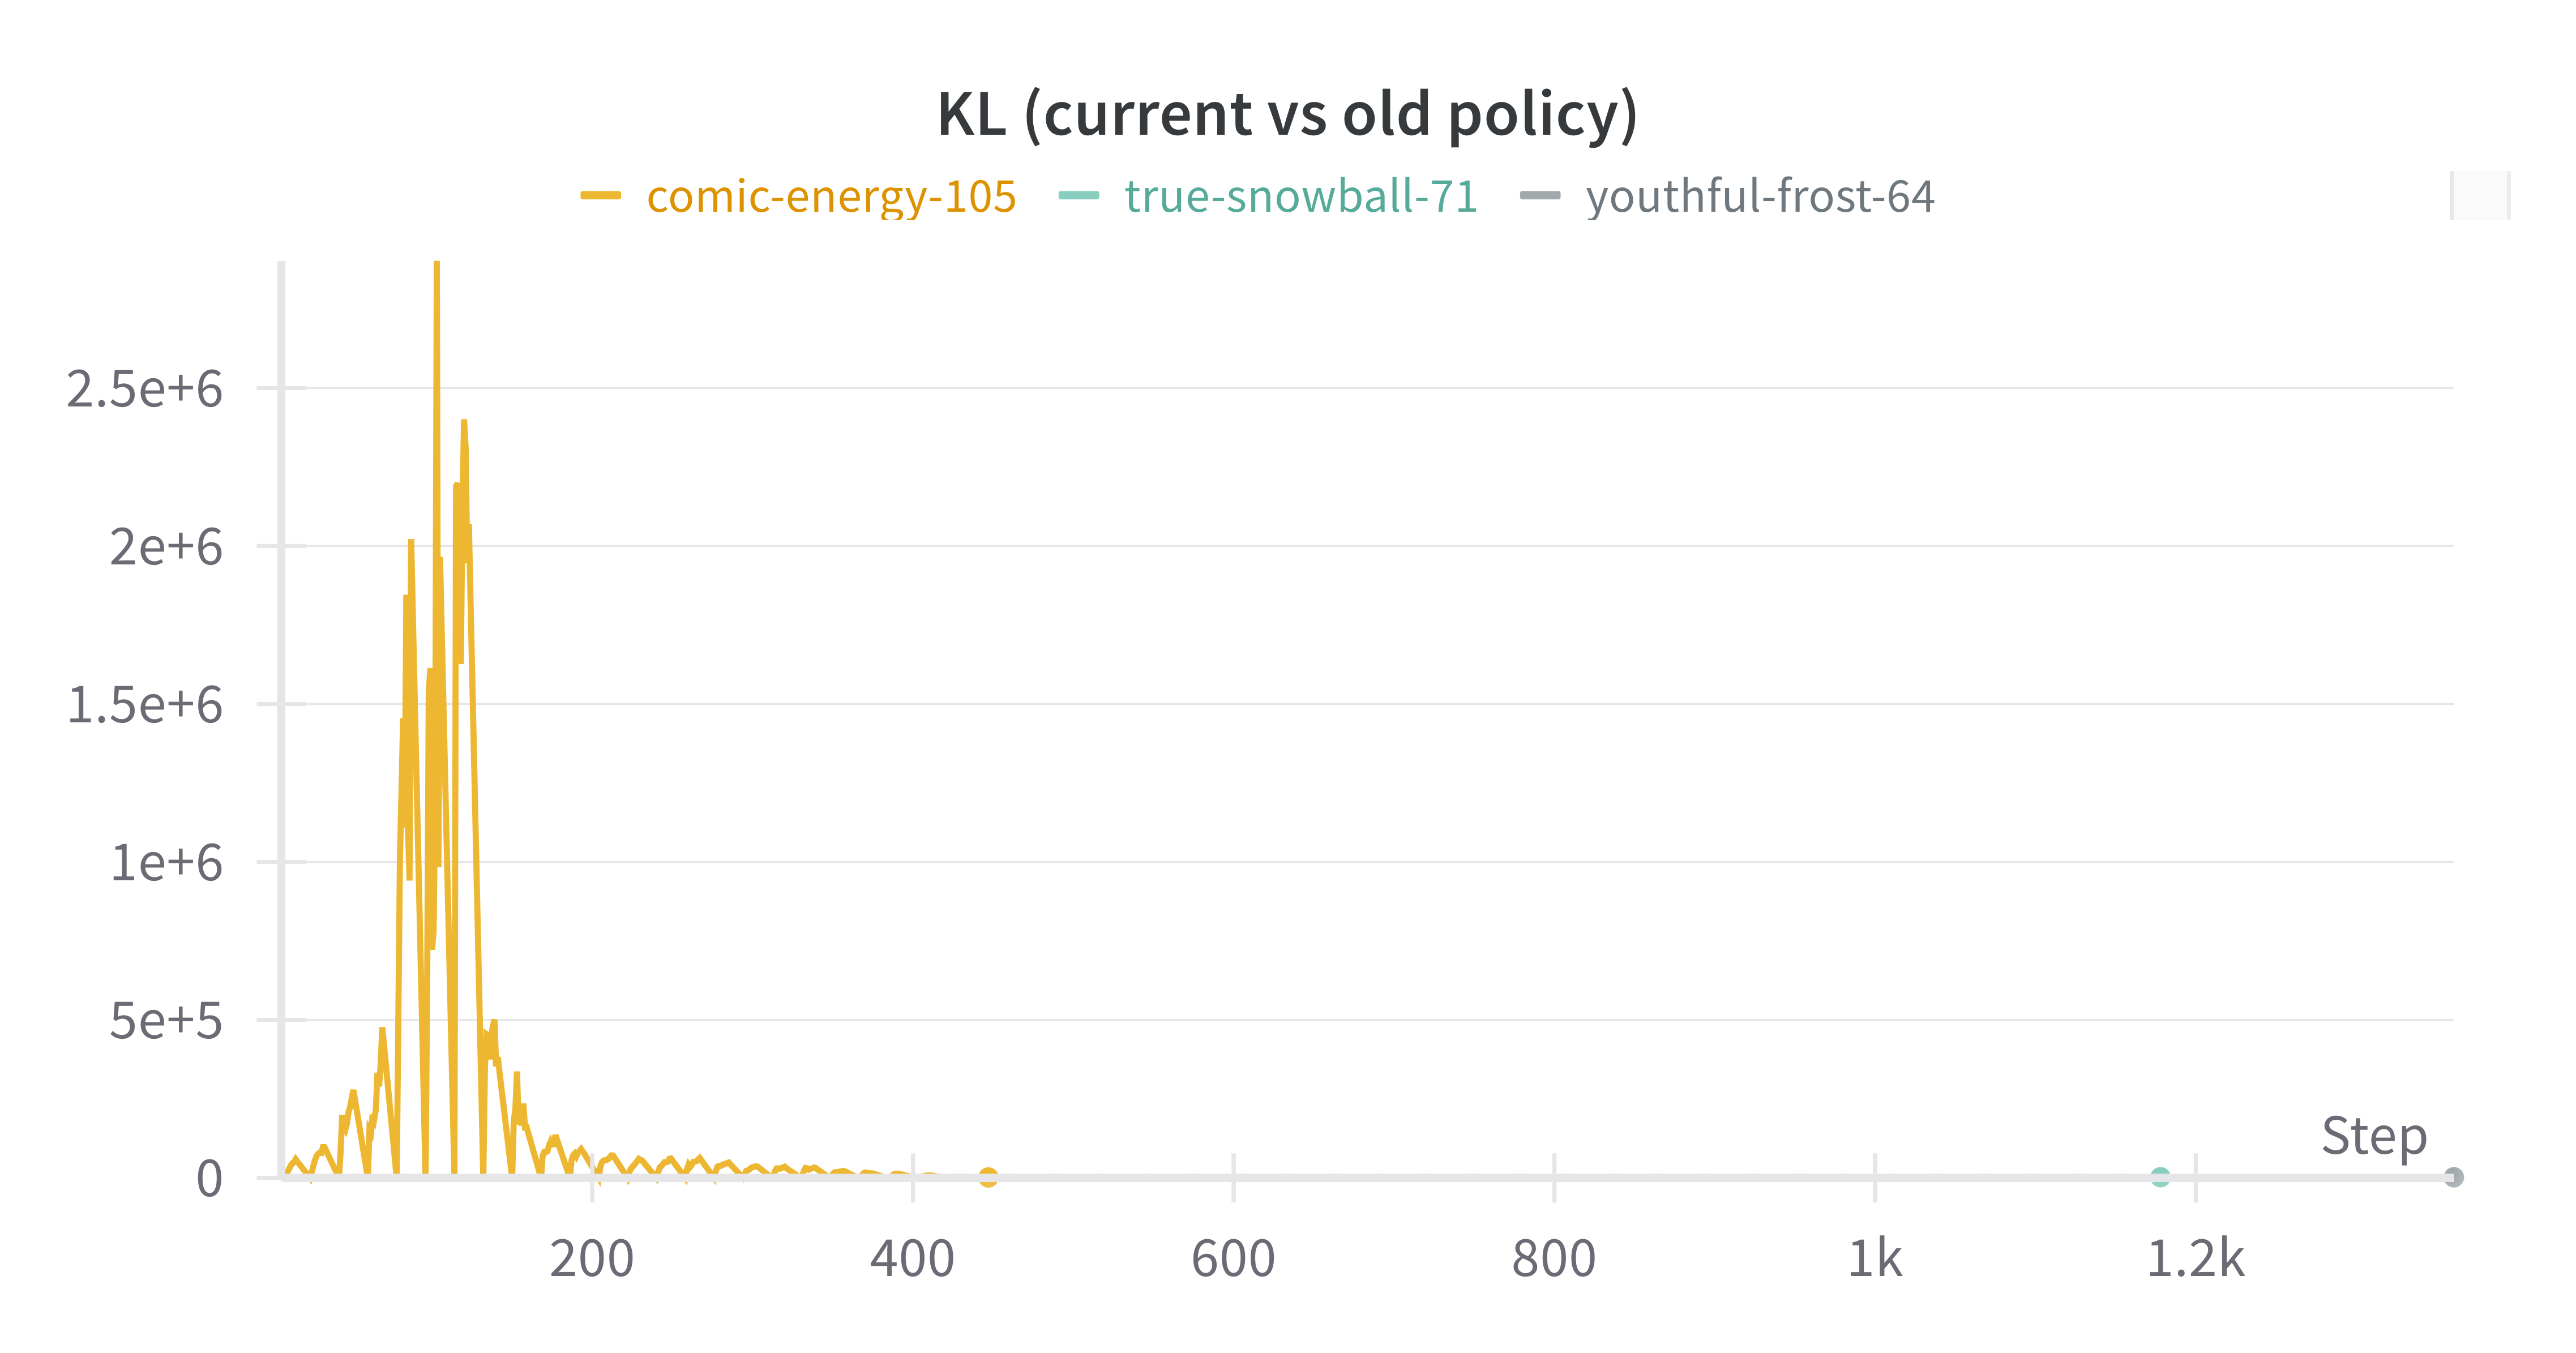
\includegraphics[width=1\textwidth]{img/results/laion-kl.png} 
  % \end{minipage}
  \vspace{-8pt}  % reduce space between caption and figure
    \captionsetup{width=\textwidth} % set the width of the caption
    \caption{\textbf{Aesthetic quality training dynamics.} \textbf{Left:} The learning rate scheduler with a linear warm-up reaching a peak learning rate of $3.64e-5$ at the first quarter of training, followed by a half-cosine decay for the remaining three-quarters. \textbf{Right:} Mean aesthetic score on the evaluation set during training. The yellow line corresponds to training with the learning rate schedule described on the left, while the other lines represent training with fixed lower learning rates of $7e-8$ and $9e-8$. Aesthetic quality requires a more complex training dynamic to achieve higher rewards.}
  \label{fig:laion-train-dynamic} % Add a proper reference for the label
\end{figure}


\noindent \textbf{Emergent effects in face generation using the LAION aesthetic predictor as a reward.} The effects observed in images generated by the DDPO-finetuned model to maximize the ``aesthetic quality'' of generated faces reflect much of the human preferences on which the LAION predictor was trained. The generated images tend to be predominantly female and appear younger. Figure~\ref{fig:aesthetic-effects} showcases these emergent effects, contrasting them with versions produced by the pretrained model. The second row displays two instances of the rejuvenation effect, with the image in the second column also undergoing a gender change. Warmer colors are also predominant, a phenomenon expected when compared to example images from the study introducing DDPO \cite{black2023training}. The hypothesis behind this warmth and sketched appearance effect is due to the preference for portraits or illustrations, which tend to be better evaluated and achieve higher aesthetic scores, thus inducing these attributes during the finetuning process. Another emergent effect is the intensity of the gaze, achieved not only through intensified eye makeup but also the ``camera position'' that captures the face, resembling a magazine cover image. Figure~\ref{fig:ddpm-to-ddpo-aesthetic} provides evidence of the transition from a sample of the pretrained model to the final checkpoint, where many of the described effects emerge, such as blondification, profiling, and rejuvenation. \\

% Effects of LAION aesthetic quality
\begin{figure}[ht]
  \centering
  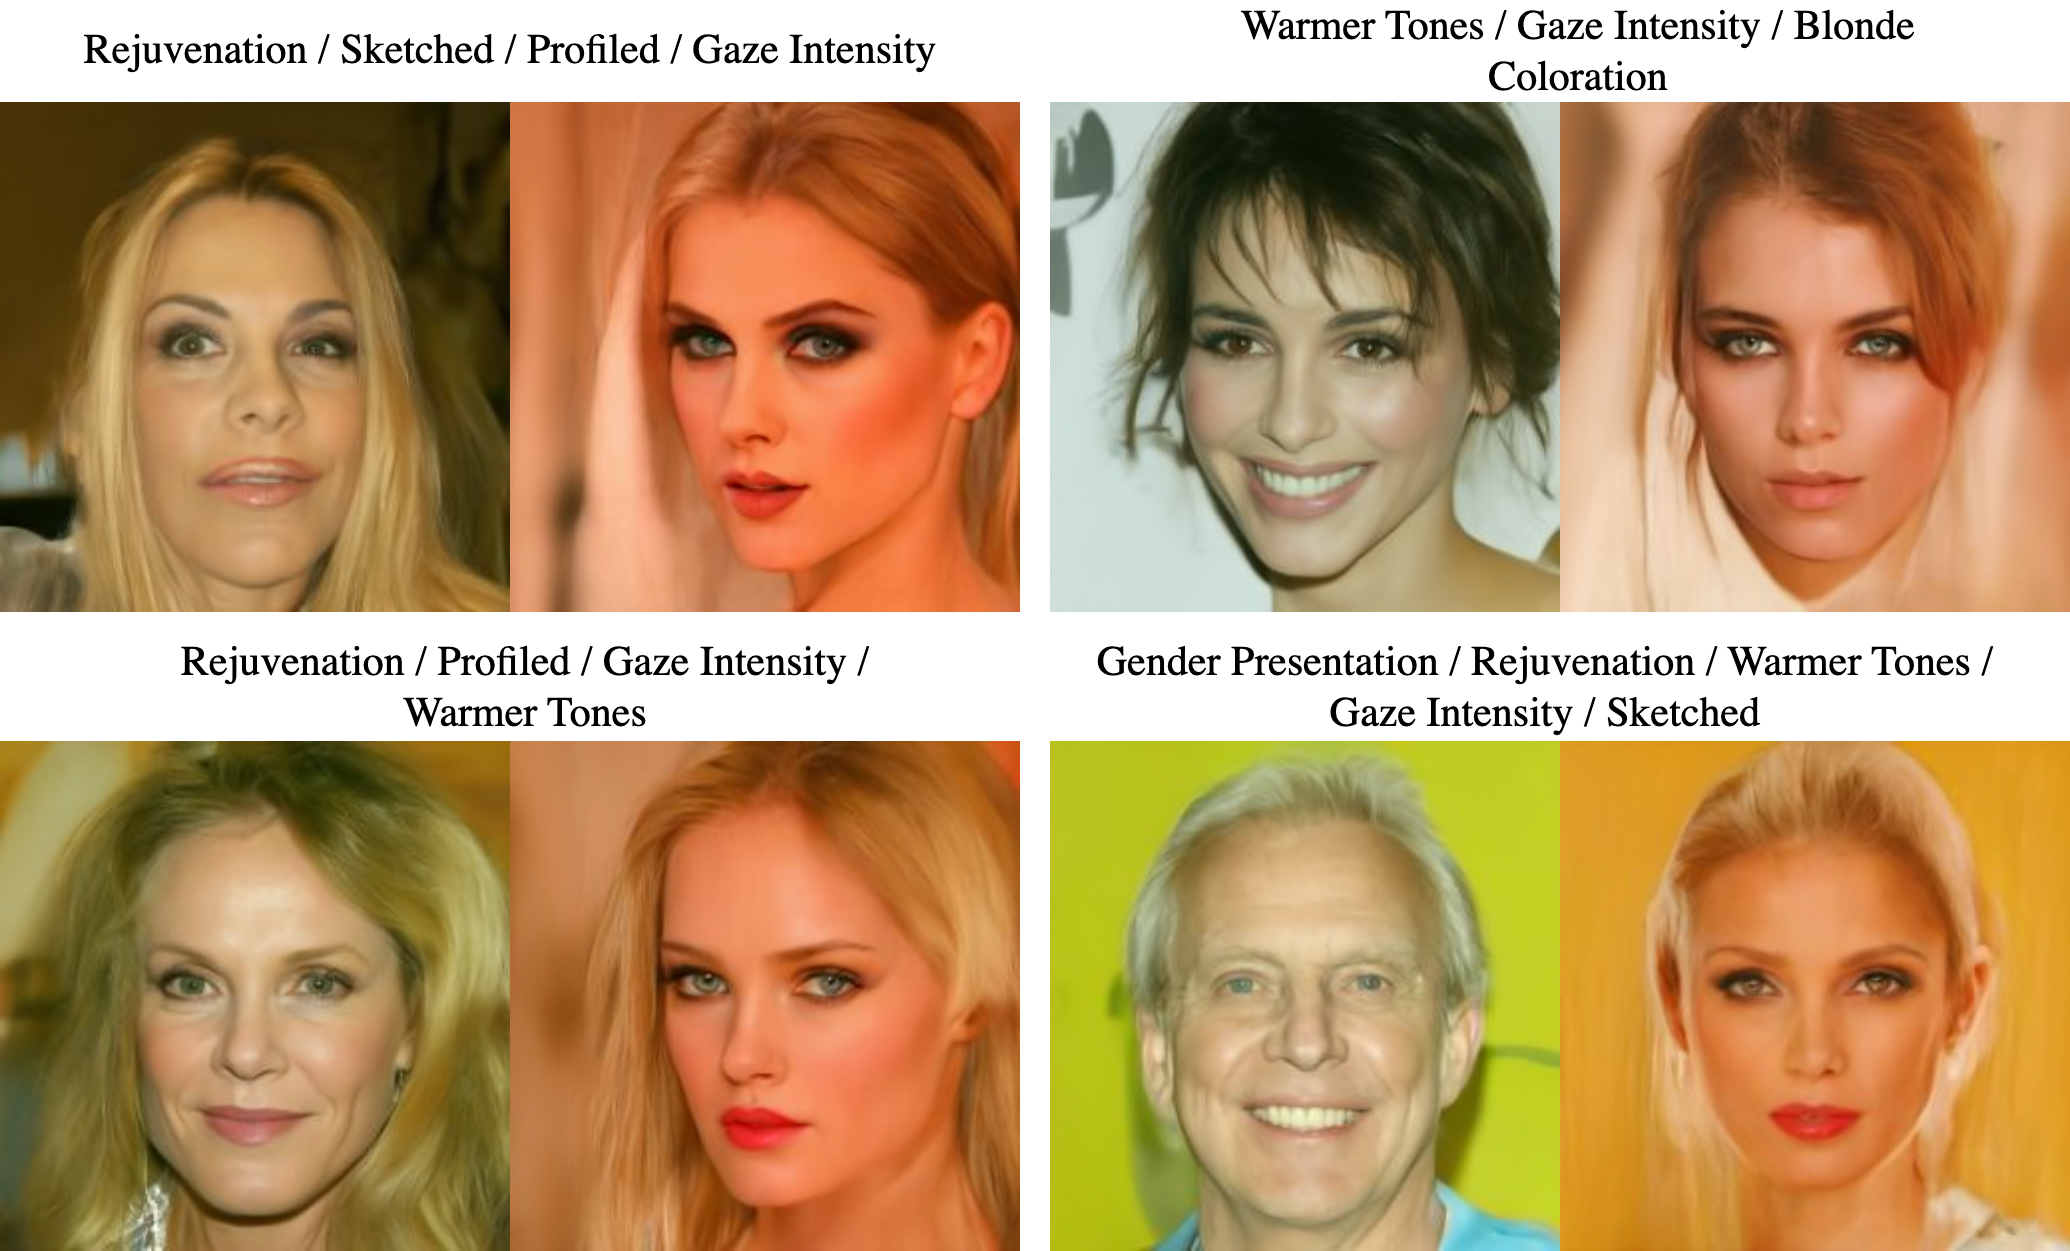
\includegraphics[scale=0.85]{img/results/aesthetic-effects.png}
  \vspace{-0pt}  % reduce space between caption and figure
    \captionsetup{width=\textwidth} % set the width of the caption
    \caption{\textbf{Emergent effects in face generation using LAION aesthetic predictor as reward.} The DDPO finetuned model, optimized for aesthetic quality, generates faces that are predominantly female, appear younger, and feature warmer tones and intensified gaze, reflecting human preferences learned by the LAION predictor. }
    \label{fig:aesthetic-effects}
\end{figure}

% Transition from DDPM to DDPO samples optimized for aesthetic quality
\begin{figure}[ht]
  \centering
  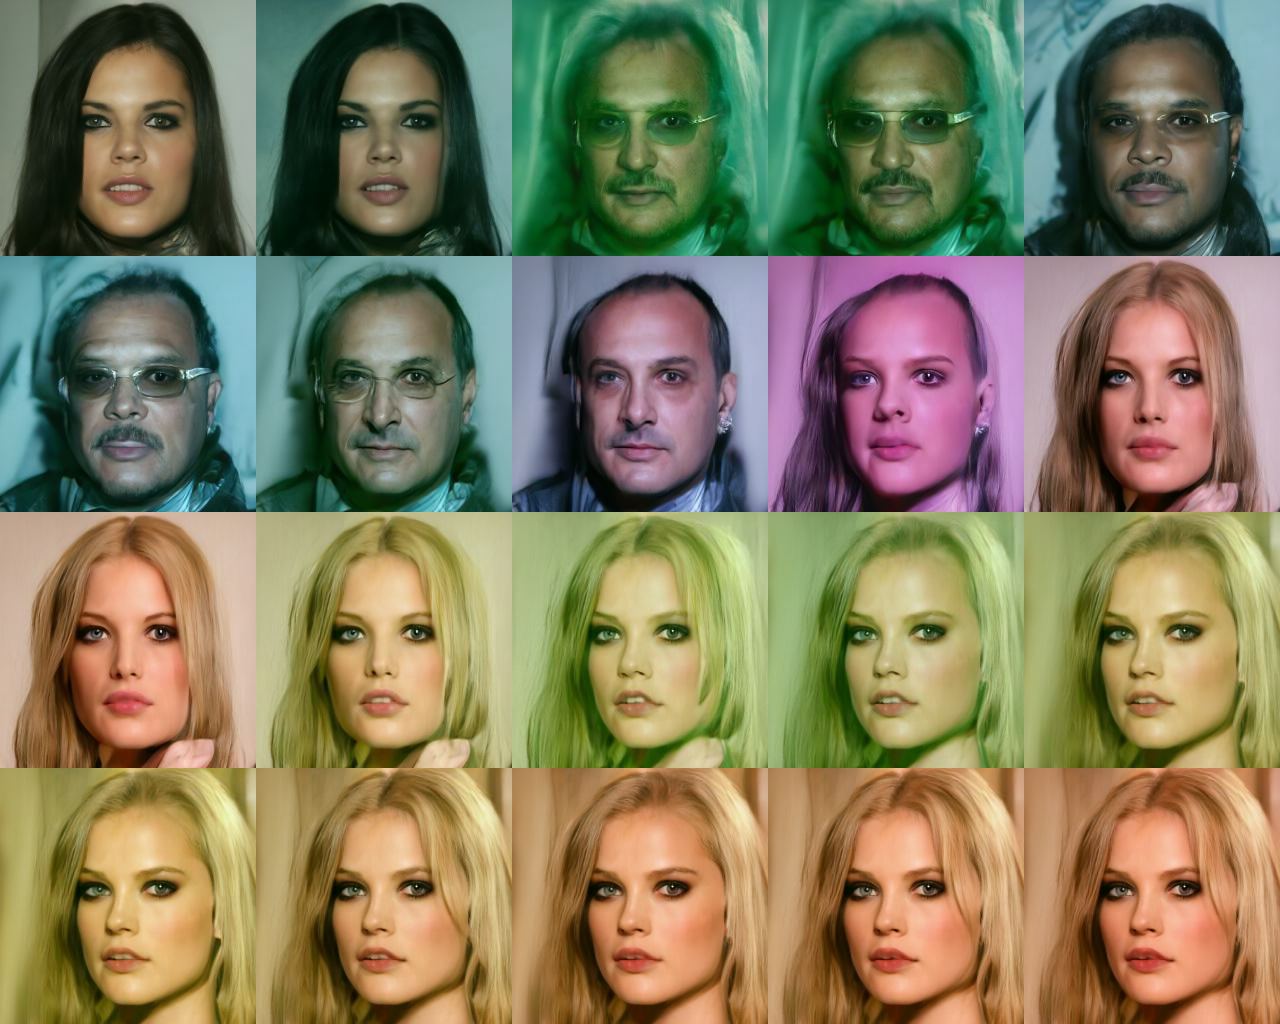
\includegraphics[scale=1.40]{img/results/laion_60.png}
  \vspace{-0pt}  % reduce space between caption and figure
    \captionsetup{width=\textwidth} % set the width of the caption
    \caption{\textbf{Example of aesthetic quality transformation during model updates}, starting with \href{https://huggingface.co/google/ddpm-celebahq-256}{\texttt{\texttt{google/ddpm-celebahq-256}}} pretrained DDPM model and optimized with DDPO to maximize aesthetic quality.}
    \label{fig:ddpm-to-ddpo-aesthetic}
\end{figure}

\noindent \textbf{Generating faces of older people}. A new task is incorporated
to demonstrate the flexibility of reinforcement learning in defining objectives. The idea is to generate faces of people over $50$ years old using images generated by a pretrained model as a starting point. The frequency
of faces of people in this age group is low, as shown in the distribution on
the left in Figure~\ref{fig:age-face-dist}. \\

\noindent It is important to note that this task is better suited to be
solved through traditional finetuning, using the same cost function employed
by the pretrained model we discussed in Section~\ref{sec:optimization-ddpm},
applied to a set of collected images of older people's faces. However, the
aim here is to demonstrate that RL can achieve this goal using only synthetic
images generated by the same model. Although this is not the most optimal 
approach, it serves as an interesting exercise to explore how even a model with a low probability of generating synthetic data with the desired attribute, such as faces of people aged 50 or older, can still produce results using the same methodological framework used in previously discussed tasks. \\

\noindent \textbf{Using a classifier to design a reward function.} A classifier is used to detect age from
facial images, trained on the FairFace dataset \cite{vitage-classifier-hf, kärkkäinen2019fairfacefaceattributedataset}. The model gives the probability that the face belong to age classes $0-2,~3-9,~10-19,~20-29,~30-39,~40-49,~ 50-50,~60-69$, and more than $70$. The reward design involves simply summing the logits of the age classes of $50$ years or older, and by using 
logits, this goal is achieved while also being more numerically stable than using the final probabilities of each class. This approach rewards the diffusion
model for generating faces of older people and disincentivizes the generation of samples with a low sum of logits in the classes of interest. We are implicitly conditioning the model to generate faces of older people by not providing direct age information as a label\footnote{An interesting experiment would be to adapt classifier-free guidance training \cite{Ho2022ClassifierFreeDG} to make the conditioning explicit while still using RL.}. \\

\noindent The results are presented in Table~\ref{tab:reward-results}, where the pre-trained model reports a logit sum of $-7.72$—--\textit{the sum of the logits of the relevant classes is considered}--—and the model finetuned with DDPO achieves a logit sum of $7.39$. It is observed that the sample trajectories increase the average reward while their dispersion decreases, indicating that the model is specializing in its objective (Figure~\ref{fig:reward_hist}, green). The age distribution of the finetuned model is shown on the right in Figure~\ref{fig:age-face-dist}. An increase in the proportion of faces of people aged $50$ or older is noted, from $6.1\%$ in the baseline to $78.7\%$ in the finetuned samples. Finally, the transition of a sample from the pretrained model to the final checkpoint is provided as evidence in Figure~\ref{fig:ddpm-to-ddpo-over50}.\\

% ViT age prediction distribution on ddpm-celebahq and dpoo-celebahq finetuned
% on logits
\begin{figure}[ht]
  \centering
  \begin{minipage}{0.5\textwidth}
    \centering
    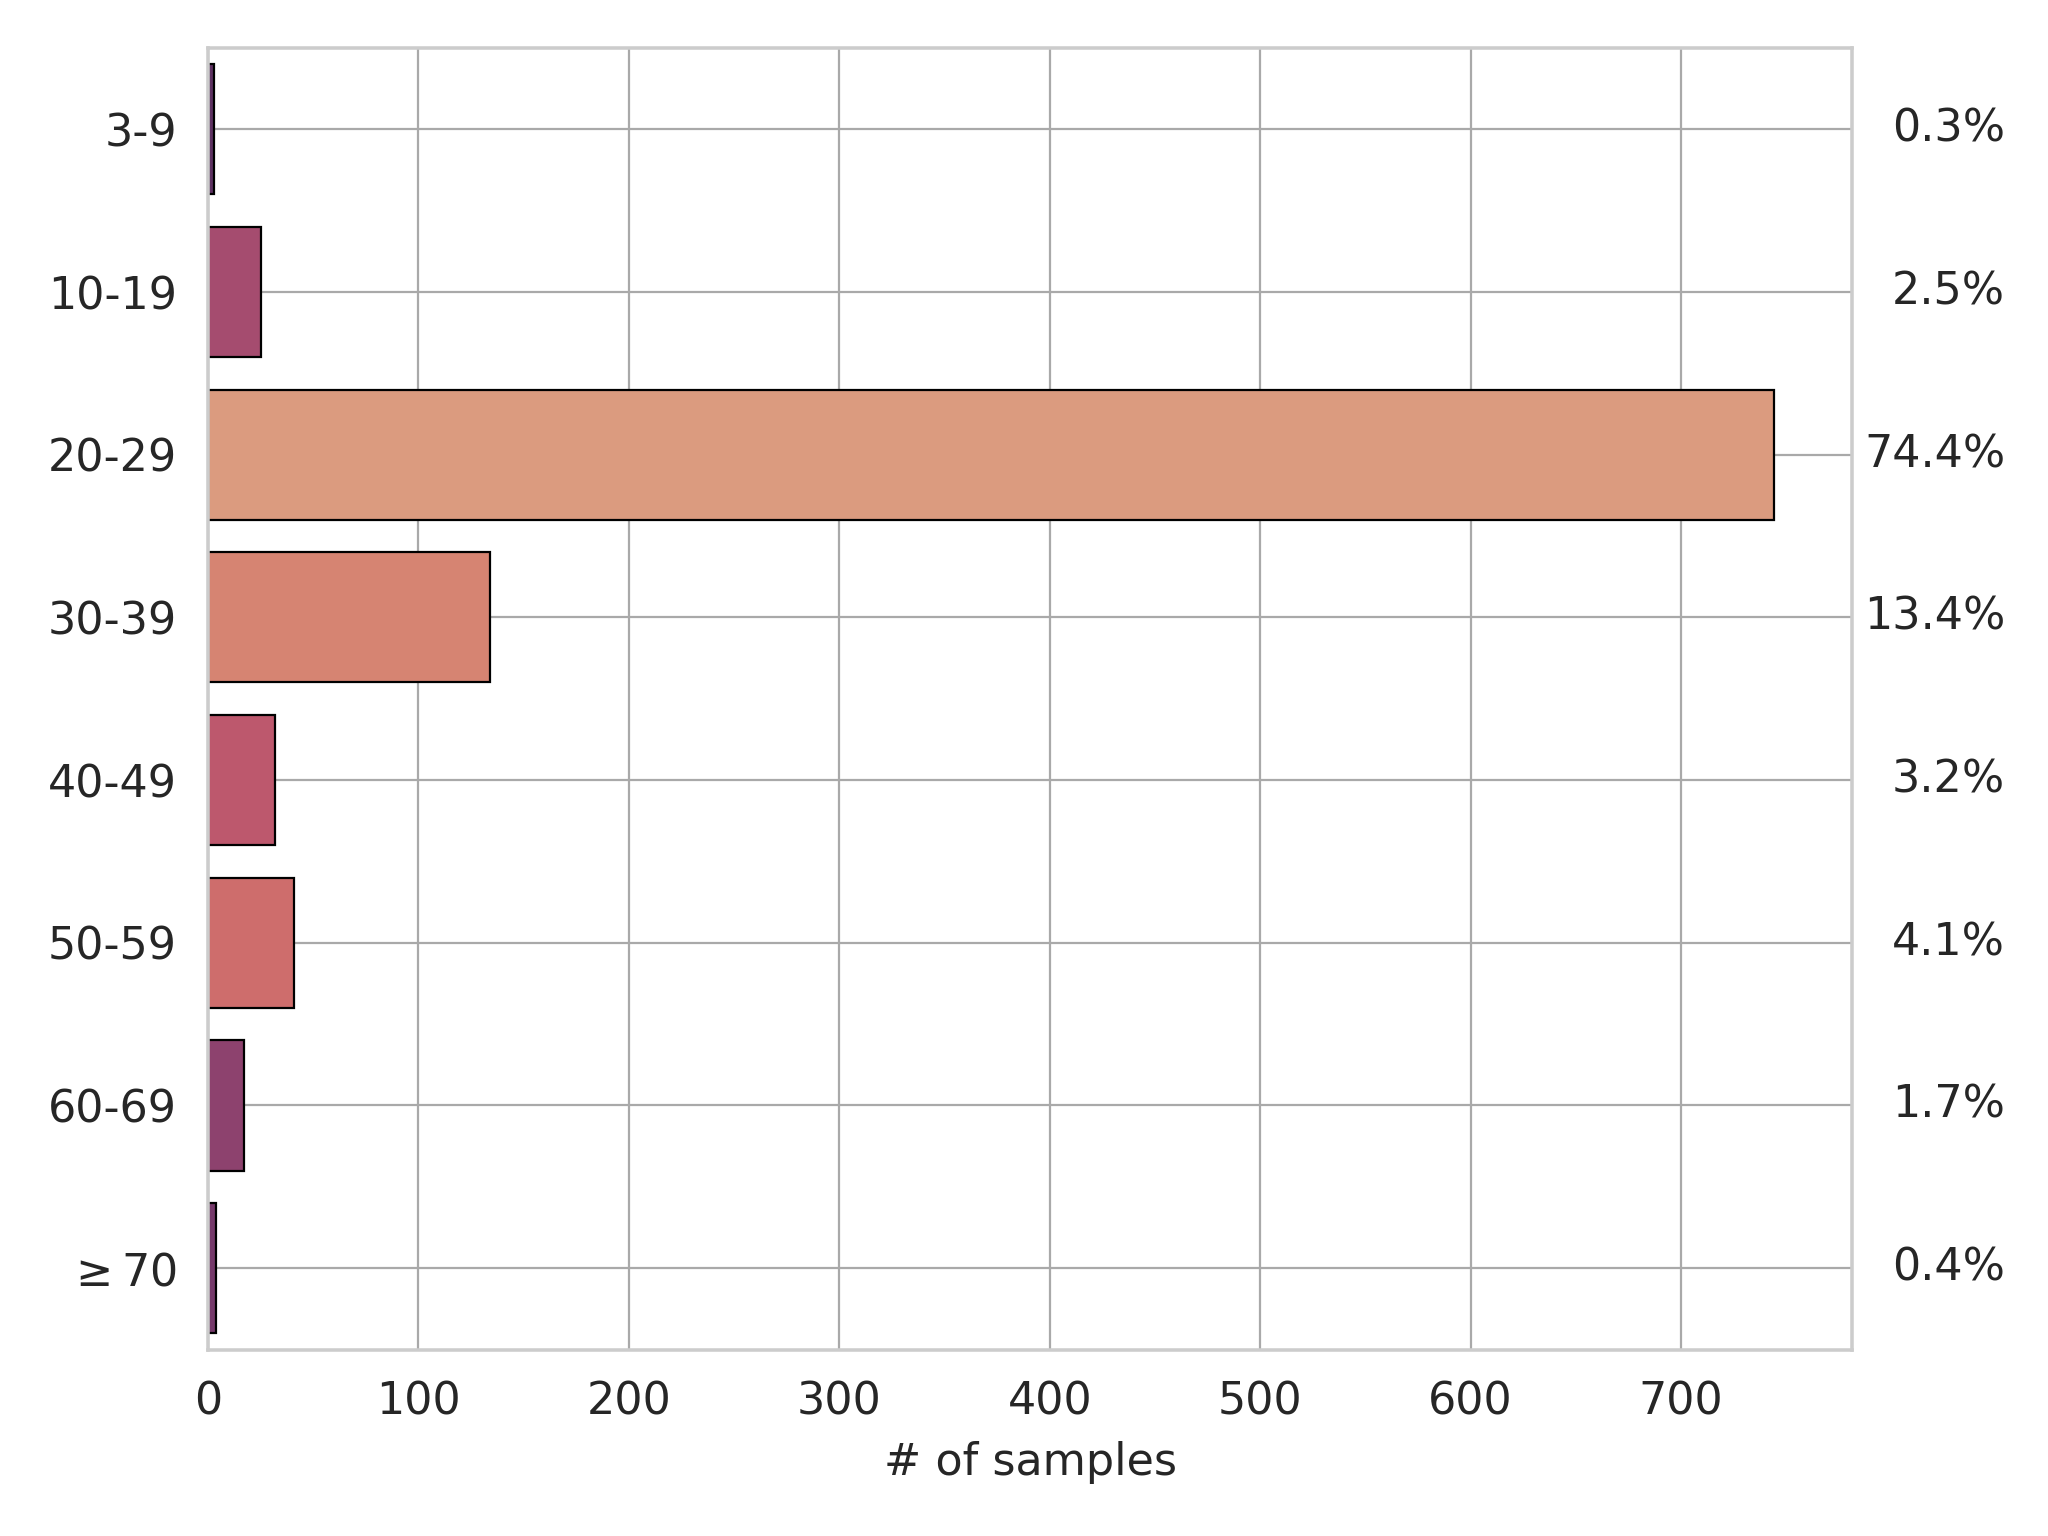
\includegraphics[width=1\textwidth]{img/results/age-dist-ddpm-celebahqsample-based-on-vit-age-preds-on-faces.png} % first figure itself
    %\label{fig:sample_figure_1}
  \end{minipage}\hfill
  \begin{minipage}{0.5\textwidth}
    \centering
    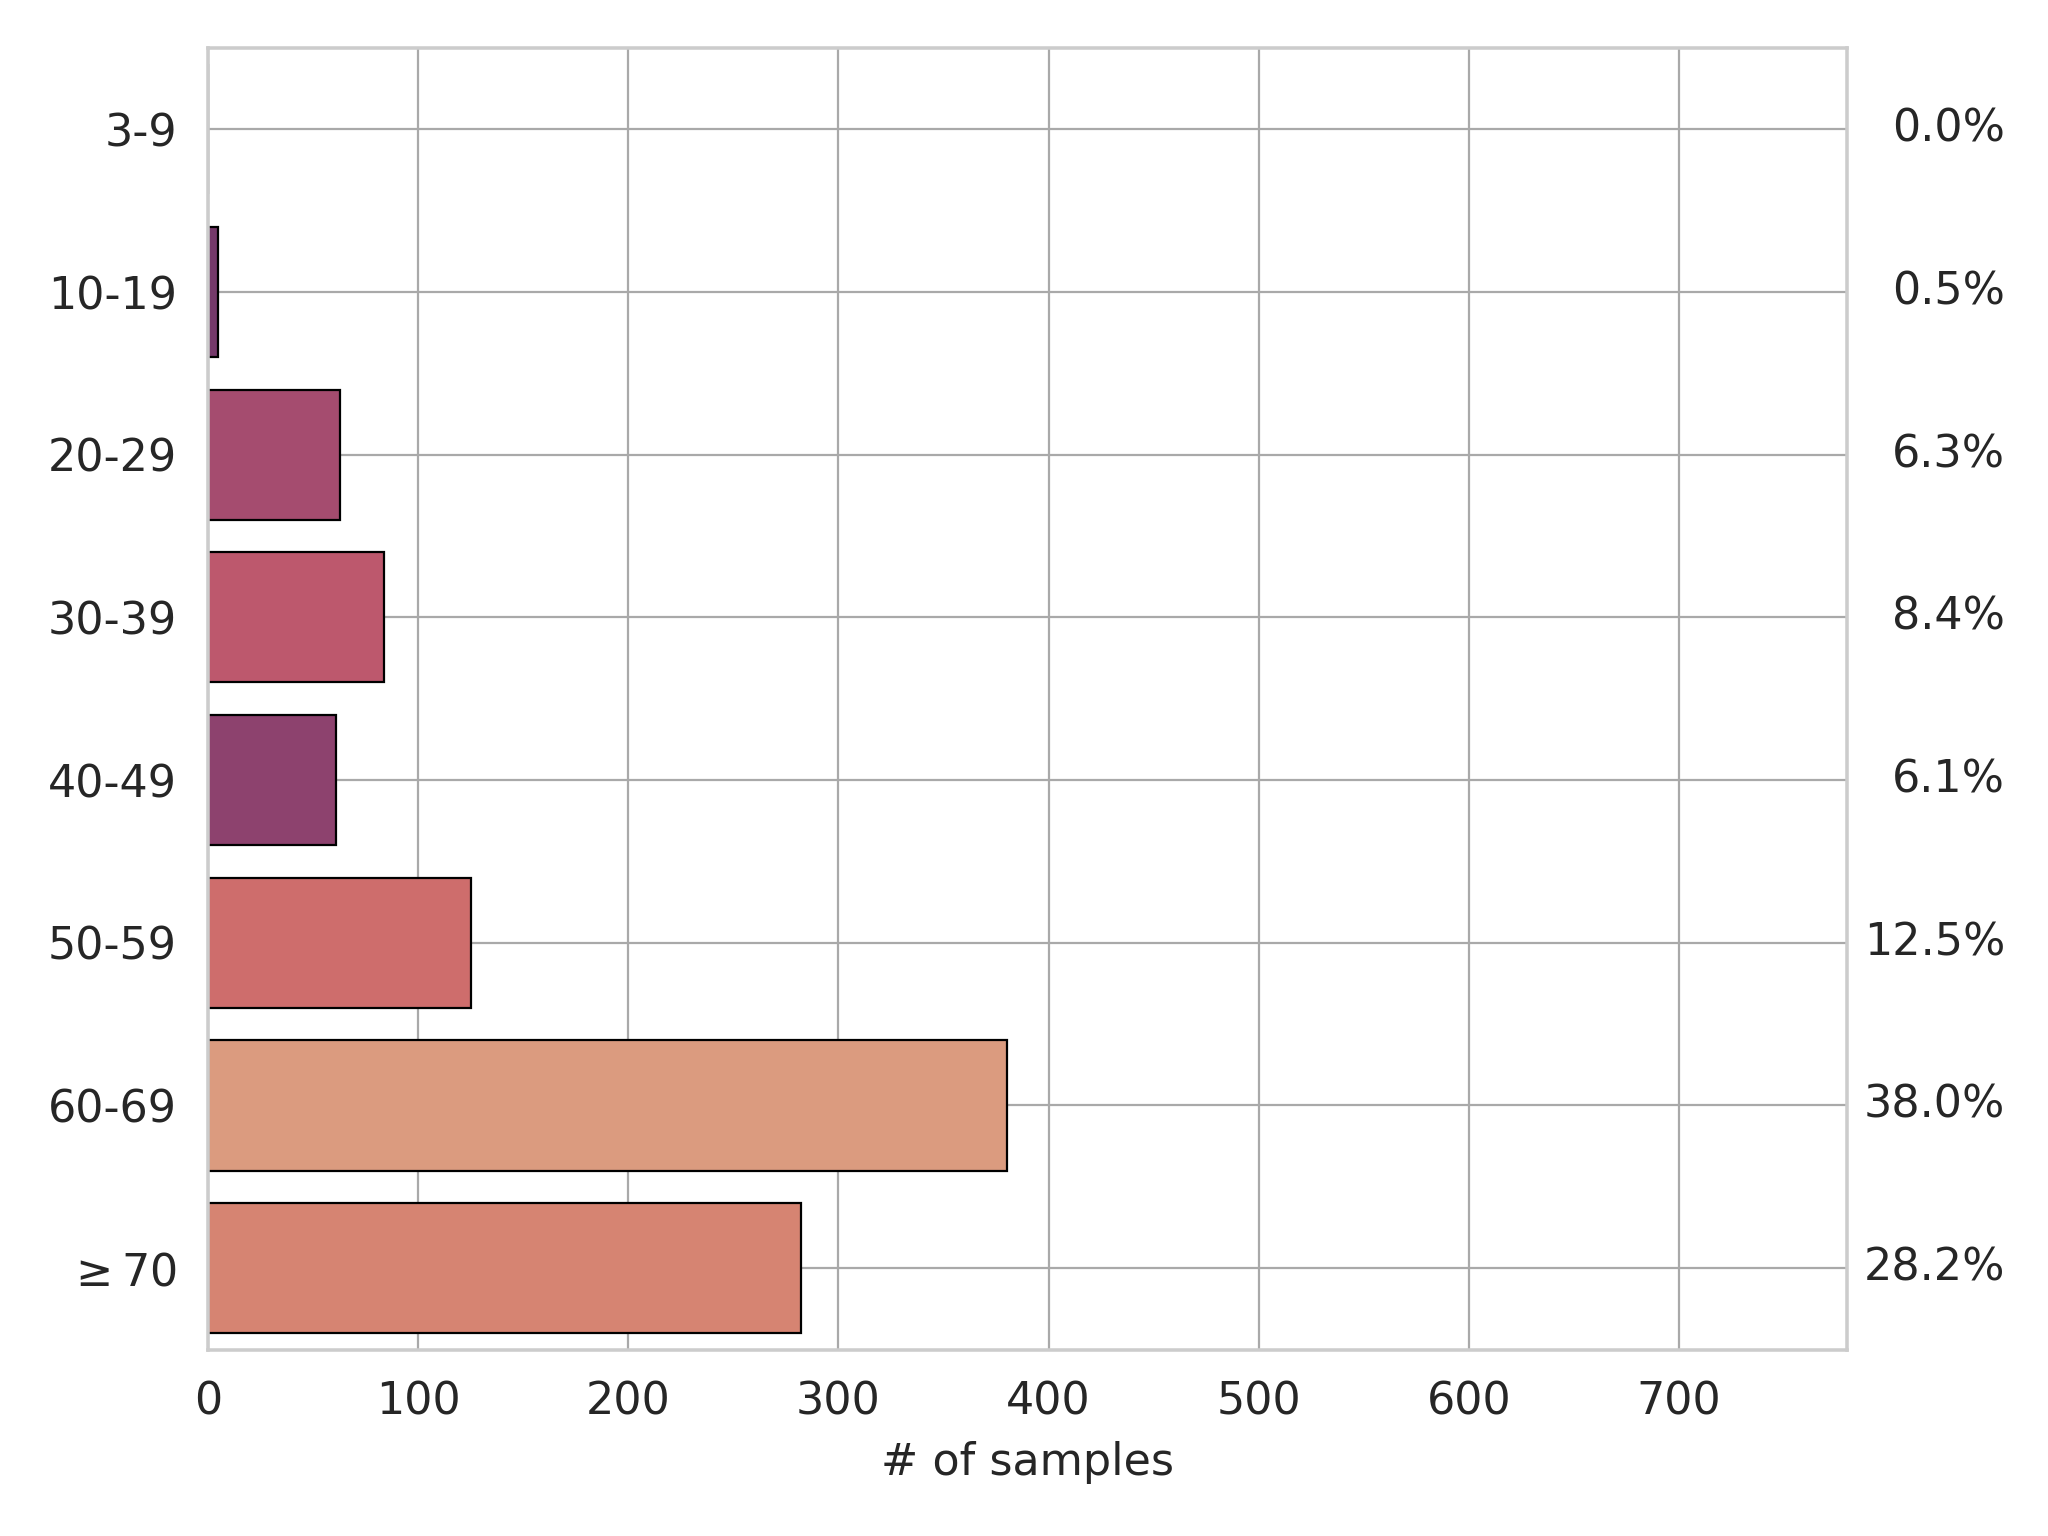
\includegraphics[width=1\textwidth]{img/results/age-dist-ddpo-celebahqsample-based-on-vit-age-preds-on-faces.png} % second figure itself
  \end{minipage}
  \vspace{-8pt}  % reduce space between caption and figure
  \captionsetup{width=\textwidth} % set the width of the caption
  \caption{\textbf{Age Distribution of Faces: DDPM (left) vs DDPO (right).} Finetuning with DDPO to maximize the logits sum for age classes 
  \texttt{$50-59$}, \texttt{$60-69$}, and \texttt{$\geq 70$}, increases the proportion of faces over $50$ years old from $6.1\%$ in the baseline to $78.7\%$ in the finetuned samples.}
  \label{fig:age-face-dist} 
\end{figure}


% Transition from DDPM to DDPO samples optimized for Task.OVER50 (ViT age classifier)
\begin{figure}[ht]
  \centering
  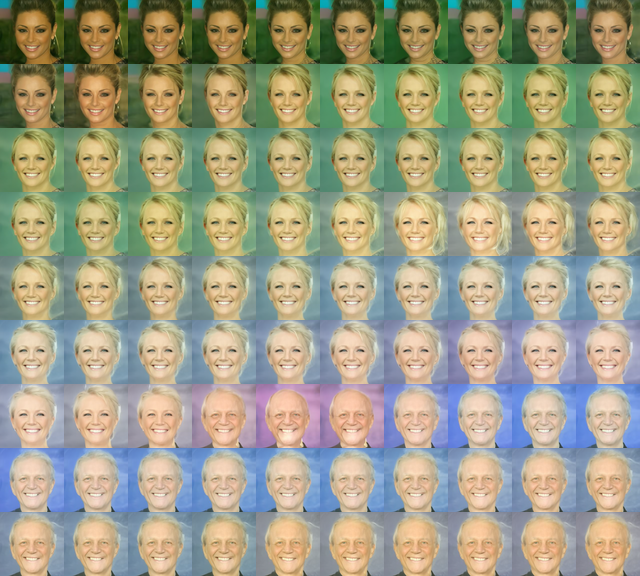
\includegraphics[scale=2.80]{img/results/over50_47.png}
  \vspace{-0pt}  % reduce space between caption and figure
    \captionsetup{width=\textwidth} % set the width of the caption
    \caption{\textbf{OVER50 transformation during model updates}, starting with \href{https://huggingface.co/google/ddpm-celebahq-256}{\texttt{\texttt{google/ddpm-celebahq-256}}}
    pretrained model and optimized with DDPO to maximize the sum of logits for classes $\geq 50$ years old using the ViT Age classifier \cite{vitage-classifier-hf}.}
    \label{fig:ddpm-to-ddpo-over50}
\end{figure}

\section{Beyond Face Generation} 

\noindent In the previous sections, we demonstrated the effectiveness of the DDPO method on a smaller pretrained model--—\textit{$114$ million parameters versus the $860$ million parameters used in the reference work (Stable Diffusion 1.4 \cite{black2023training})}--—to generate images of faces, optimizing for four different downstream tasks. To verify the robustness of the method, experiments were conducted using another pretrained model with a completely different visual semantics, focusing not on face generation but on images of buildings, specifically trained on churches from a subset of the \textbf{L}arge-scale \textbf{S}cene \textbf{UN}derstanding challenge dataset, also known as LSUN \cite{Wang_2017}. The base model, \href{https://huggingface.co/google/ddpm-church-256}{\texttt{\texttt{google/ddpm-church-256}}}, trained using the same DDPM methodology \cite{ho2020denoising} outlined in Algorithm 1, was finetuned for the first three downstream tasks, excluding \texttt{OVER50} for obvious reasons. \\

\noindent Figure~\ref{fig:visual-comparison-ddpo-church} offers a visual comparison between four samples from the pretrained model and their versions generated by the finetuned models across the respective tasks. The images are generated from the same initial noise to facilitate comparison and highlight the effects induced by the reward functions. It is noteworthy that the definition of the churches is not always of high quality; in the first image of the pretrained model's sample quadrant, a building is visible that might be a church, but it is not immediately obvious. One hypothesis for why this model generates lower-fidelity images is the complexity of details and variations in scene images, such as those of churches, compared to other concepts like the elements needed to generate faces. This likely results in the model not capturing details as effectively, thereby reducing its generative capacity. The remaining three images from the pretrained model samples exhibit higher levels of definition, clearly showing churches of different styles. \\

\noindent The results for the compressibility and incompressibility reward tasks are shown in Table~\ref{tab:reward-results}, where the average size of images generated by the pretrained model after JPEG compression is reported to be $29.57$ kB. These images are generally larger than those generated by the pretrained model for celebrity faces, due to the greater number of elements and details in scene images like those of churches, making compression more challenging. In the case of the compressibility reward, the average image size generated by the model finetuned with DDPO is $10.62$ kB, while for the incompressibility task, the average size is $50.21$ kB. This represents a $64\%$ reduction in image size when optimizing for compressibility and a $70\%$ increase in image size when optimizing for incompressibility, relative to the model's initial generative capabilities. \\

\noindent Analyzing the effects of the reward functions as seen in the samples in Figure~\ref{fig:visual-comparison-ddpo-church}, the primary emerging effect when maximizing compressibility is the prevalence of night skies and overall darker images. Notably, even as the images darken, light sources such as the moon or artificial illumination emerges, as seen in the first row of images. The effects of optimizing the incompressibility task include an overall increase in image illumination and the generation of elements like trees, grass, or bushes with numerous leaves. In this regard, the two samples in the first column of the incompressibility examples show signs of over-optimization, as the effect degrades the visual semantics of the reference churches. Transitions from pretrained to finetuned models are presented in Figure~\ref{fig:ddpm-to-ddpo-church}; the first row provides another example of how the darkening effect in the skies emerges, but also of how artificial illumination emanates from the building itself. Conversely, the second row shows the addition of strong green tones resembling grass and the transformation of distant mountains into something more akin to trees. The cloudy sky begins to detail more but eventually results in an excess that diminishes the sense of density and realism. A similar degradation occurs in the building, which becomes less realistic in the final two images. \\

\noindent Regarding aesthetic quality in Figure~\ref{fig:visual-comparison-ddpo-church}, there is a generalized saturation of details, with trees appearing in $3$ out of the $4$ images. For example, in the second image of the first row, we can see several trees and bushes surrounding the church. Another detail visible in this image, as well as in the others in the group, are the lines on the building's walls, which give the impression that the material is stone. This could be because images of buildings with such details tend to be rated higher in aesthetic quality by the LAION aesthetic predictor. The fourth image is more grandiose compared to its original version, with more detailed and numerous clouds, the church dome replaced by a tower, and the building protruding from the left side of the original image replaced by a tree with branches. Additionally, the interplay of light and shadow gives the impression that the image was taken at sunset. In terms of quantitative results, Table~\ref{tab:reward-results} reports an average aesthetic score of $4.77$ for the pretrained LSUN model, which increases to $5.13$ after optimizing for aesthetic quality. Finally, a transition image between the pretrained model and checkpoints during parameter tuning is presented in the third row of Figure~\ref{fig:ddpm-to-ddpo-church}. This transition suggests converting the church in the figure into an image where the background contains houses and other buildings. The hypothesis for this effect is that many images containing churches also include a view of the city, as seen in the first pretrained model sample in Figure~\ref{fig:visual-comparison-ddpo-church}, which may explain why the transition results in an image saturated with elements that blur the distinction of individual buildings but collectively resemble a city or cluster of buildings. \\

% Visual Comparison google/ddpm-church-256 vs finedtuned models
\begin{figure}[ht]
  \centering
  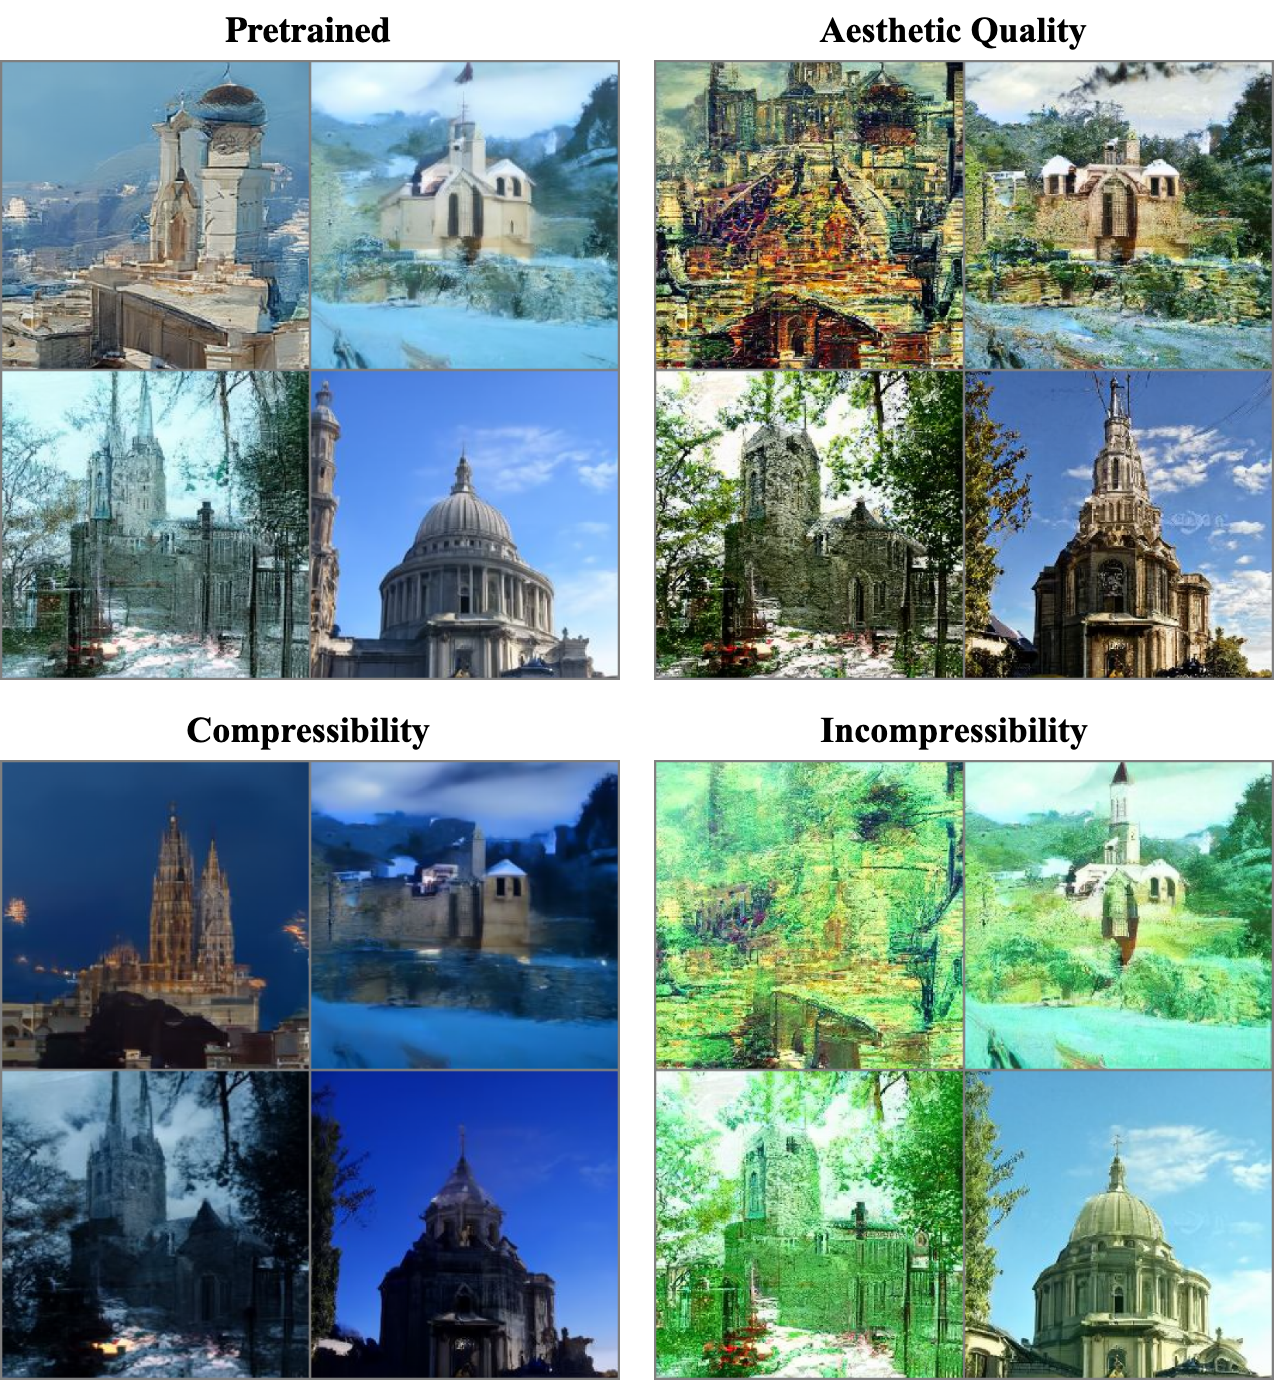
\includegraphics[scale=0.85]{img/results/visual-comparison-church-results.png}
  \vspace{-0pt}  % reduce space between caption and figure
    \captionsetup{width=\textwidth} % set the width of the caption
    \caption{\textbf{DDPM pretrained model's samples vs DDPO finetuned samples.} Qualitative depiction of the effects of RL finetuning on different reward functions using \href{https://huggingface.co/google/ddpm-church-256}{\texttt{\texttt{google/ddpm-church-256}}}
    pretrained model. Additional samples are provided in Appendix~\ref{appendix:additional-church-samples}.}
    \label{fig:visual-comparison-ddpo-church}
\end{figure}


% Church transitions on JPEG compressibility, incompressibility, and aesthetic
% quality
\begin{figure}[ht]
  \centering
  \includegraphics[scale=0.57]{img/results/transitions_churchs.png}
  \vspace{-15pt}  % reduce space between caption and figure
    \captionsetup{width=\textwidth} % set the width of the caption
    \caption{\textbf{Transition from DDPM to DDPO finetuned.} Finetuning transitions on different reward functions for the \href{https://huggingface.co/google/ddpm-church-256}{\texttt{\texttt{google/ddpm-church-256}}} pretrained model, shown top-to-bottom: JPEG compressibility, incompressibility, and aesthetic quality.}
    \label{fig:ddpm-to-ddpo-church}
\end{figure}

\section{Discussion \& Limitations}

\noindent\textbf{Overoptimization and diversity samples.} Despite the benefits 
of optimizing diffusion models using reinforcement learning, reward overoptimization remains a significant challenge. This issue arises when the model excessively exploits the reward function \cite{gao2023scaling}, leading to a lack of diversity in the generated samples. In severe cases, this can degrade image semantics, resulting in a model that fails to achieve practical utility. \\

\noindent To understand and visualize reward overoptimization in the context of this work, we extract CLIP \cite{radford2021learning} features from two sets of images that share the same initial seed and noise. One set is generated by the \href{https://huggingface.co/google/ddpm-celebahq-256}{\texttt{google/ddpm-celebahq-256}} (as mentioned in section \ref{sec:empirical-analysis}), and the other set is generated using a DDPO checkpoint \href{https://huggingface.co/alkzar90/ddpo-aesthetic-celebahq-256}{\texttt{alkzar90/aesthetic-celebahq-256}} optimized for aesthetic quality. We then  project these image features into a $2$ dimensional embedding space using t-SNE \cite{van2008visualizing} to visualize the samples. \\

\noindent As shown in Figure~\ref{fig:clip-emb-ddpo-vs-ddpm}, we observe that the samples optimized for aesthetic quality cluster near the sample with the highest aesthetic score from the DDPM set (illustrated in Figure~\ref{fig:sample-trajectories}). This occurs because the model reinforces samples with higher aesthetic quality, generating more of these samples until the
model concentrates on a very specific high-reward region, ultimately collapsing into a single mode. \\

\begin{figure}[ht]
  \centering
  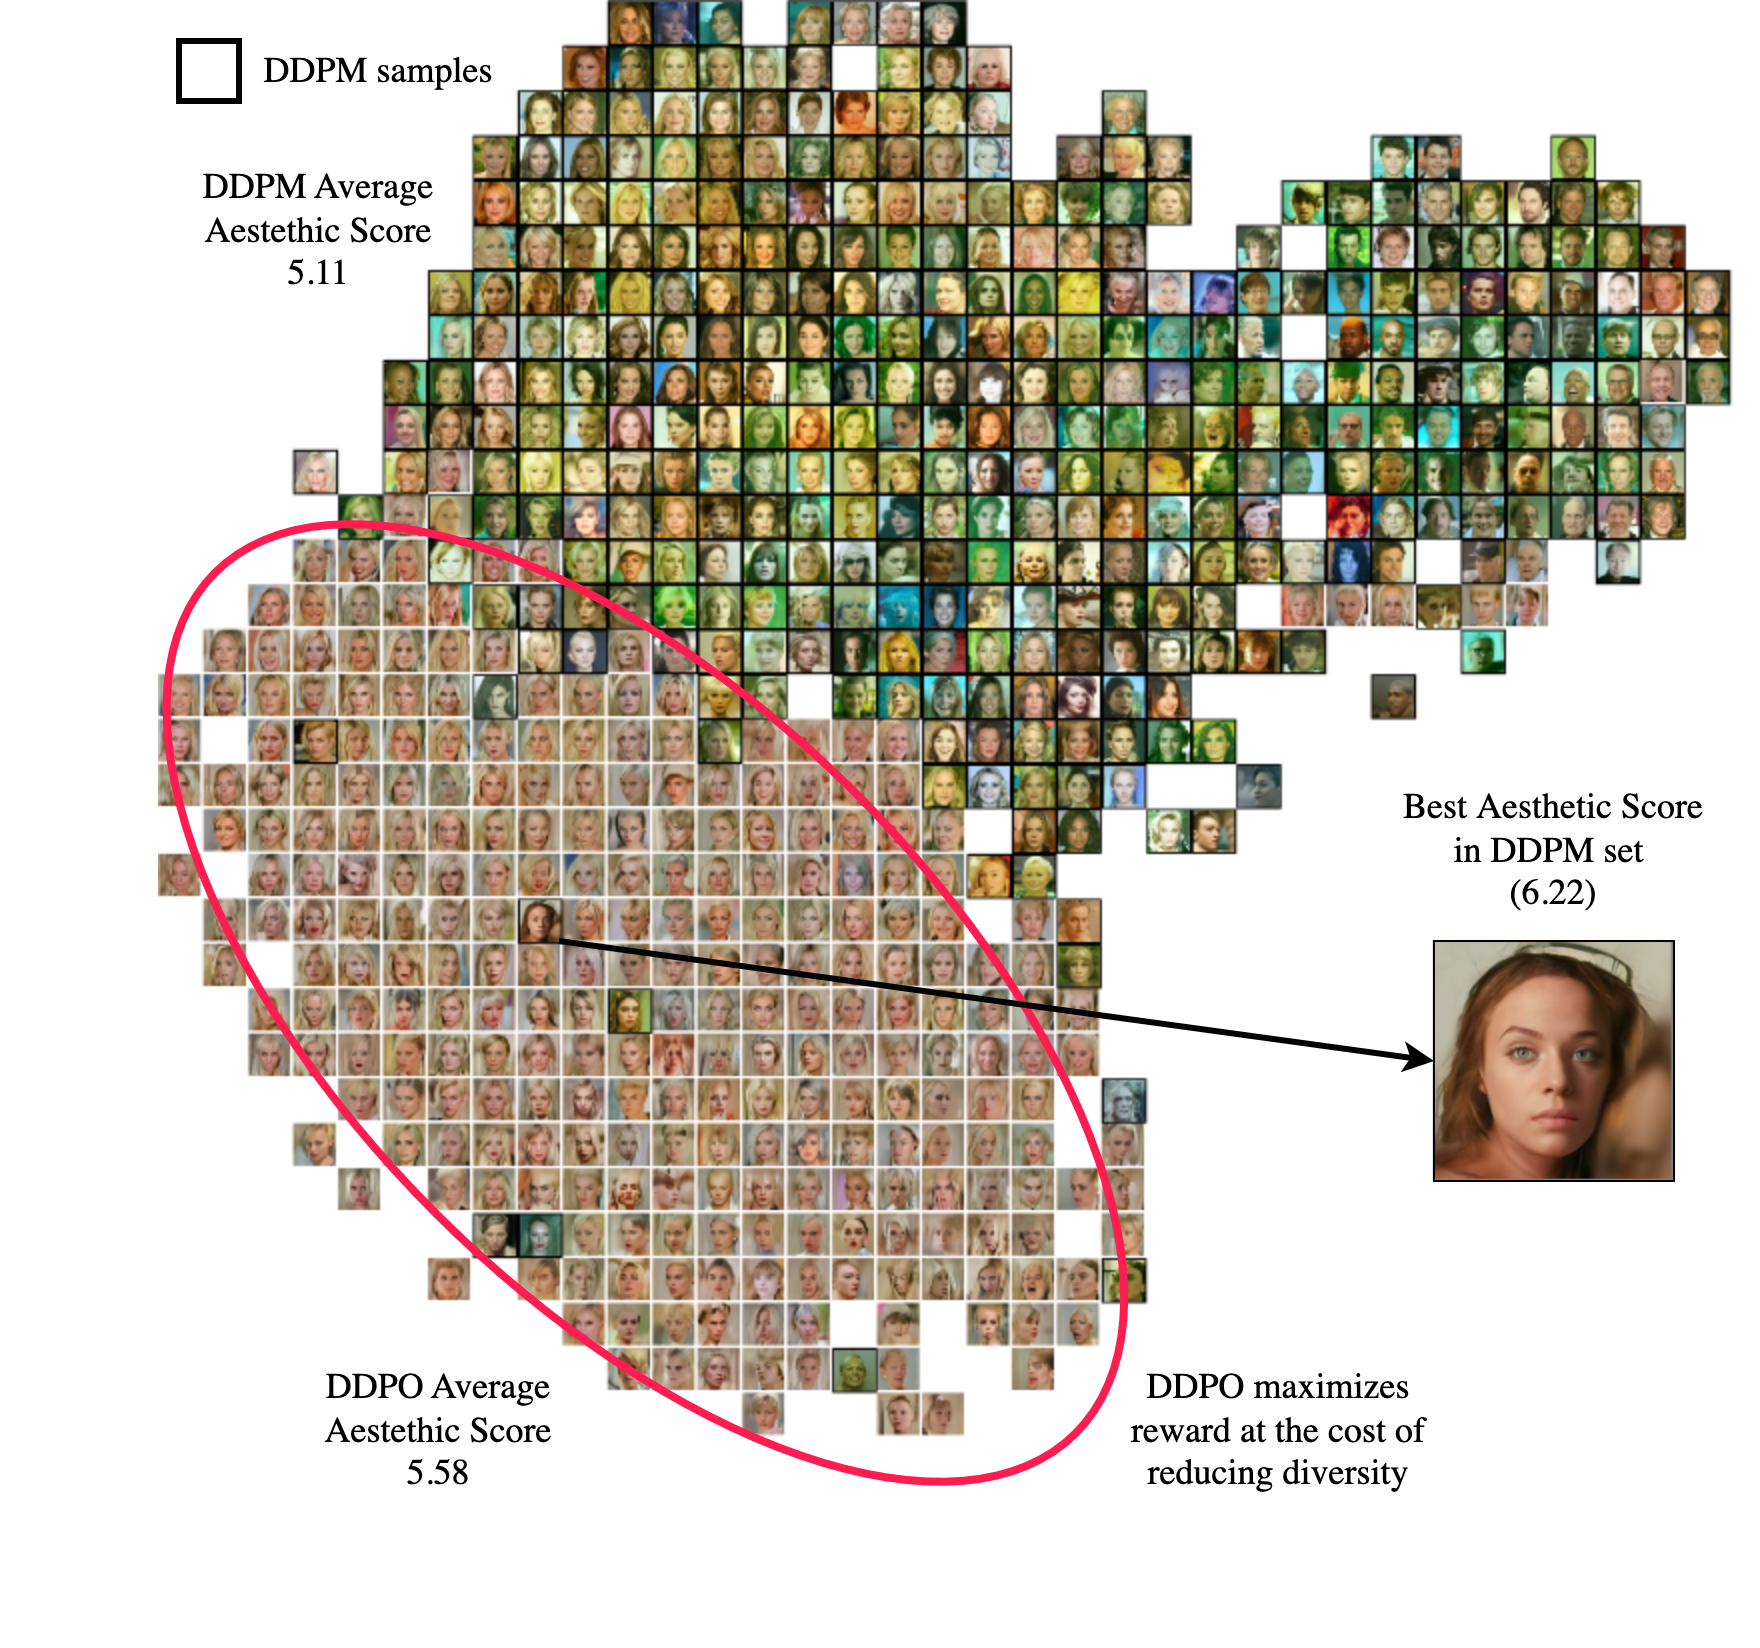
\includegraphics[scale=0.72]{img/results/emb-space-ddpo-vs-ddpm2.png}
  \vspace{-40pt}  % reduce space between caption and figure
    \captionsetup{width=\textwidth} % set the width of the caption
    \caption{\textbf{CLIP Feature Embedding Space: DDPM vs. DDPO Samples.} Both sets of samples were generated from the same seed. Notably, samples optimized for aesthetic quality cluster near the highest aesthetic score sample from the DDPM pretrained model (Figure~\ref{fig:sample-trajectories}), illustrating a clear \textit{\textbf{mode collapse effect}}.}
    \label{fig:clip-emb-ddpo-vs-ddpm}
\end{figure}

\noindent\textbf{Broader impact.} Research into finetuned diffusion models with reinforcement learning offers significant advantages in gaining precise control over image generation, unlocking various practical applications. These models can be tailored to produce highly specific outputs, allowing for the generation of images that meet exact requirements in fields such as entertainment, virtual reality, medical imaging, and design. For instance, in the healthcare industry, these models could aid in creating accurate simulations for surgical planning or training, providing a safe and controlled environment for practice. In the creative industries, they can enhance the ability to generate unique and high-quality visual content, facilitating the development of realistic video games or films. The capacity to finetune these models with RL also means they can adapt to new styles or features as needed, offering businesses and researchers flexible tools that evolve with their requirements. \\

\noindent However, alongside these advantages, there are critical ethical concerns related to the use of diffusion models, particularly regarding bias and fairness. When trained on datasets containing biases, such as those related to gender, geography, or ethnicity, these models risk perpetuating and amplifying these biases in their outputs. It doesn’t require much attention to notice that the mode collapse effect, previously demonstrated, is a clear example of preference bias affecting the reward model. Samples with higher rewards are concentrated in profiles of women with white skin and blond hair (see more samples in Figure~\ref{fig:ddpo-aesthetic-samples}). While reinforcement learning with human feedback (RLHF) techniques can be used to align the model with operator preferences and mitigate this issue, they can also exacerbate the problem or lead to unexpected consequences by aligning with subjective objectives or preferences that may not be representative. \\

\section{Future Work}

\noindent \textbf{Avoid mode collapse.} One consequence of the overoptimization problem discussed previously is the mode collapse effect, which leads to a lack of diversity in the samples. Mode collapse is a common issue in generative models. Can we develop a method to avoid this effect in the context of diffusion models? An interesting research direction is to gain control over the diffusion chain process to influence and block certain features during reward finetuning. Identifying and managing local features in images to unlock alternative high-reward areas can help prevent mode collapse or at least reduce its impact without compromising sample diversity, effectively controlling the trade-off between overoptimization and diverse samples. \\

\noindent \textbf{Measure diversity.} Exploring the use of Vendi Score \cite{friedman2023vendiscorediversityevaluation, pasarkar2024cousinsvendiscorefamily}, a metric inspired by statistical ecology to evaluate the diversity of samples, could provide insights into how to algorithmically improve sample generation \cite{hemmat2024improvinggeodiversitygeneratedimages} and mitigate the mode collapse problem. \\

\noindent \textbf{A benchmark dataset for evaluation.} Evaluation is difficult and not straightforward for assessing the effectiveness of a method. Does the method generalize to other models trained on different datasets? How can we evaluate the performance of the model in a more robust way? How many downstream tasks provide robustness in the generalization of a method? These questions must be addressed with equal effort as in the application of RLHF for large language models. An immediate effort is to define a set of downstream tasks that cover a wide range of objectives and preferences, on both smaller and larger models. This includes providing access not only to the checkpoints used to report results but also to the samples and reward evaluations. \\

\noindent \textbf{Exploit the intermediate states rewards.} Empirical analysis of the reward signal during the sample generation process shows that the reward signal is more informative in denoised samples than in noisy ones (Section~\ref{sec:empirical-analysis}). Can we take advantage of intermediate states to explore the space more efficiently? Introducing an agent that can build intermediate denoised modifications worth exploring could increase the data generated in a useful way for DDPO or alternative preference algorithms. \\
